%----------
\section{Solutions des exercices du chapitre 6}
%----------

\subsection*{Solution exercice 6.1 - qualité de l'usinage de lentilles optiques}

\begin{wrapfigure}[20]{l}[0pt]{6.7cm}
   \centering
   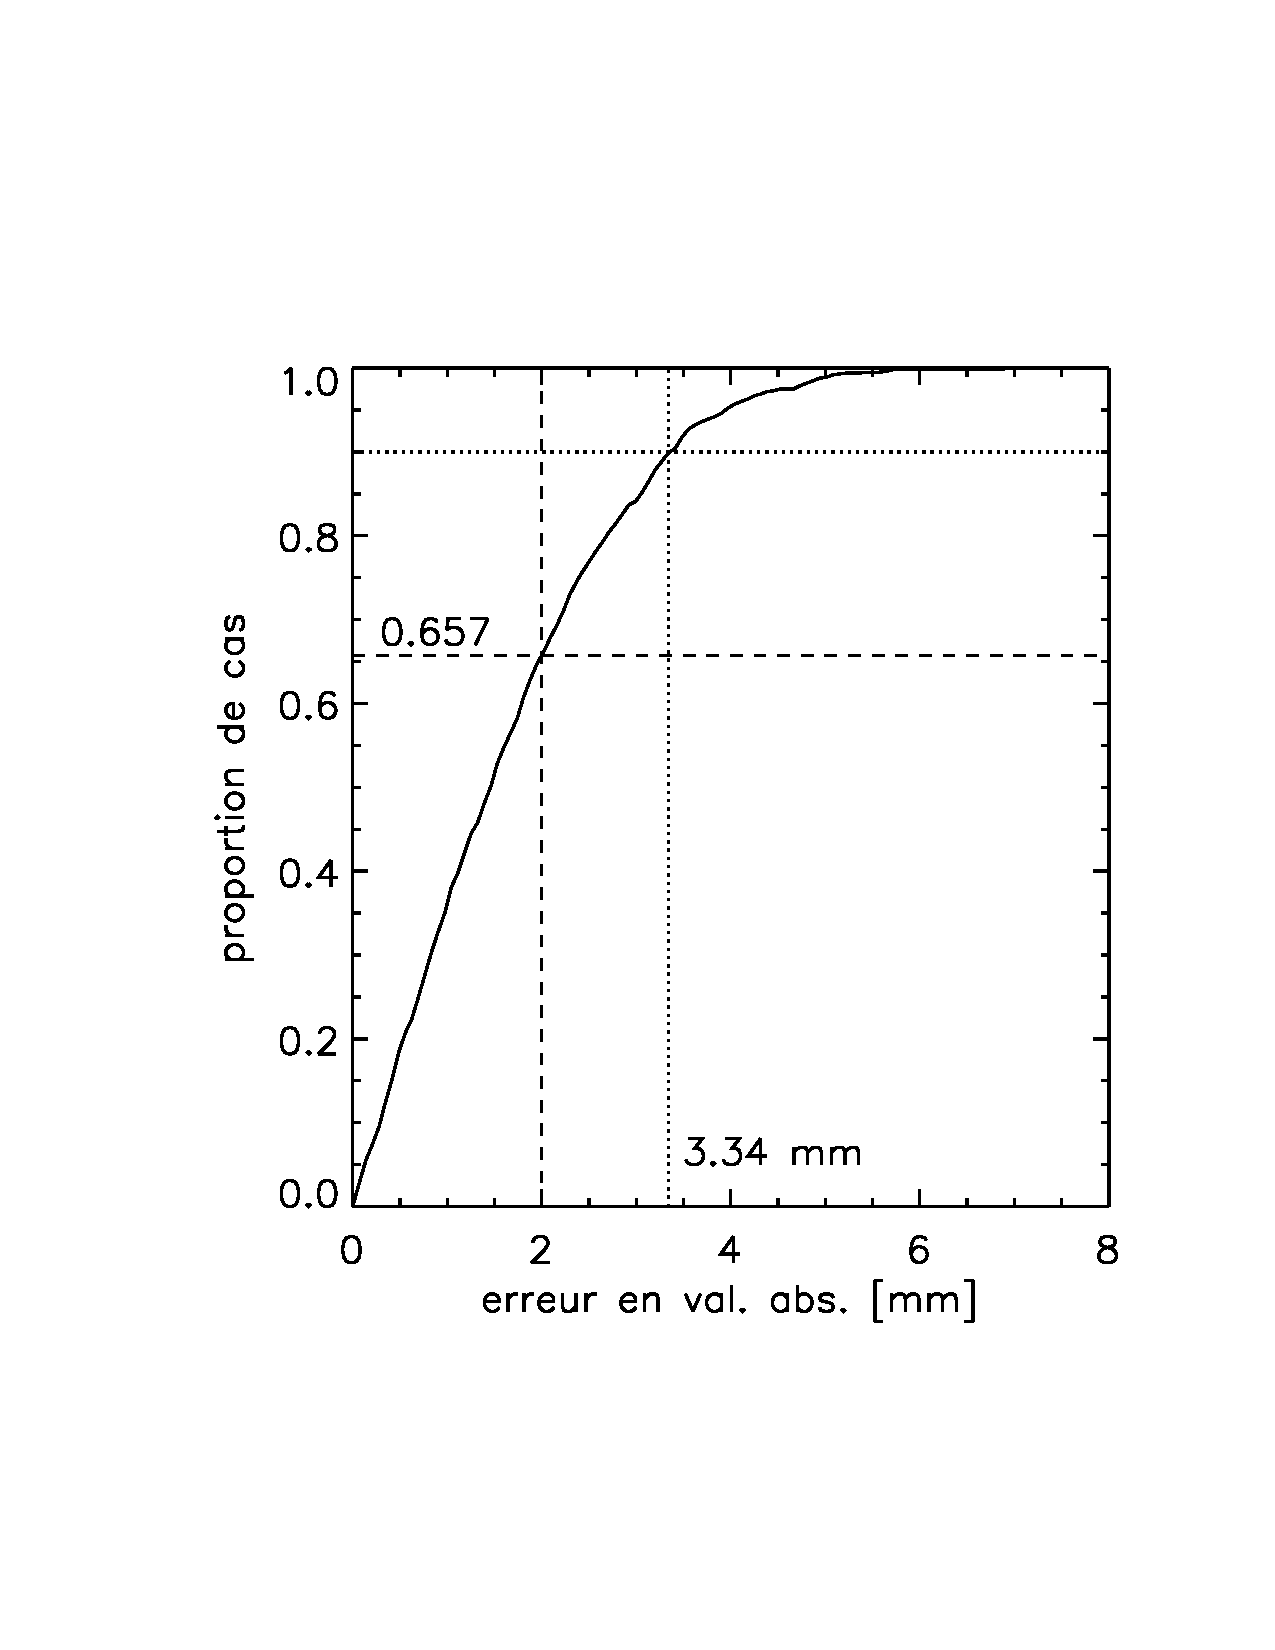
\includegraphics[width=6.5cm]{fig/Serie1_exe1_cumulativeDisribution.pdf}
   \caption{Proportion de lentilles ayant une erreur sur la focale inférieure ou égale à la valeur indiquée en abscisse.}
   \label{fig:01}
\end{wrapfigure}
On charge les données dans \texttt{matlab} avec la commande \texttt{load} - consultez le \textit{user manual} pour toute question relative à l'utilisation de \texttt{matlab}. En tant que futurs ingénieurs, vous devez êtres capable de vous débrouiller seuls avec un logiciel en lisant le manuel de l'utilisateur.

\textbf{Q1~:} Il suffit de calculer le nombre de fois que la donnée est dans l'intervalle 98-102 mm, par rapport au nombre total de données; on trouve qu'il y a 675 cas sur 1000 soit 67.5\% des lentilles qui sont acceptables;

Pour savoir quelle est l'erreur d'usinage si on accepte 90\% des lentilles, il suffit de construire l'histogramme cumulé, jusqu'à l'erreur maximale, ce qui donne la courbe de la figure~\ref{fig:01}, puis on cherche par tâtonnement la valeur correspondant à 90\% du maximum de l'histogramme cumulé, soit 3.34 mm. Par conséquent, si on accepte une erreur de 3.34 mm sur la focale, alors jusqu'à 90\% des lentilles sont acceptables.

\textbf{Q2~:} $\langle R\rangle=49.991$ mm, $\text{med}(R)=49.987$ mm, $\text{mode}(R)=49.95$ mm, $\sigma_R=1.029$ mm; on remarque que les trois valeurs de la moyenne, de la médiane et du mode sont très proches les unes des autres, on doit donc s'attendre à un histogramme très symétrique autour de la moyenne.

\textbf{Q3 et Q4~:} On trouve $\beta_1=-0.0426758$ et $\gamma_2=-0.265687$; l'histogramme est par conséquent très symétrique, et très légèrement plus étroit qu'une gaussienne pure.

\textbf{Q5~:} Pour construire la tableau des fréquences, il n'y a rien d'autre à faire que de compter le nombre de cas dans chaque classe, en fonction du nombre de classes. L'intervalle entre le maximum (52.9633 mm) et le minimum (46.5538 mm) de $R$ est de 6.4095 mm, par conséquent, pour respectivement 5, 10, 20 et 40 classes, les largeurs de classe $\Delta R$ sont 1.28190 mm, 0.640950 mm, 0.320475 mm et 0.160238 mm. En triant, on arrive aux tableaux de fréquences donnés en table~\ref{tab:cl}, et aux histogrammes de la fig.~\ref{fig:hist}.

\textbf{Q6 et Q7~:} Il est clair que l'histogramme à 20 classes est celui qui véhicule le mieux la structure de la distribution, pratiquement une gaussienne, sans alourdir le graphique avec trop de données. L'histogramme à 10 classes pourrait encore convenir, mais 5 classes, c'est clairement trop peu. Par ailleurs, si votre collègue trouve une réponse légèrement différente de la votre, c'est parce que calculer des métriques à partir d'un histogramme est toujours une approximation - à moins que l'histogramme ne soit construit à partir d'une infinité de mesures - ce qui n'est jamais le cas.

\begin{table}[p]
\footnotesize
\caption{Tableaux des fréquences pour 5, 10 ,20 et 40 classes.}
\begin{center}
\begin{tabular}{cccccccc}
5 classes [mm] & fréq. & 10 classes [mm] & fréq. & 20 classes [mm] & fréq. & 40 classes [mm] & fréq. \\\hline
46.5538-47.8357 &  17 & 46.5538-47.1948 &   2 & 46.55380-46.87427 &   1 & 46.55380-46.71404 &  1 \\
47.8357-49.1176 & 187 & 47.1948-47.8357 &  15 & 46.87427-47.19475 &   1 & 46.71404-46.87427 &  0 \\
49.1176-50.3995 & 438 & 47.8357-48.4767 &  61 & 47.19475-47.51522 &   4 & 46.87427-47.03451 &  0 \\
50.3995-51.6814 & 312 & 48.4767-49.1176 & 126 & 47.51522-47.83570 &  11 & 47.03451-47.19475 &  1 \\
51.6814-52.9633 &  46 & 49.1176-49.7586 & 204 & 47.83570-48.15617 &  21 & 47.19475-47.35499 &  0 \\
         total & 1000 & 49.7586-50.3995 & 234 & 48.15617-48.47665 &  40 & 47.35499-47.51522 &  4 \\
                    & & 50.3995-51.0405 & 201 & 48.47665-48.79712 &  55 & 47.51522-47.67546 &  7 \\
                    & & 51.0405-51.6814 & 111 & 48.79712-49.11760 &  71 & 47.67546-47.83570 &  4 \\
                    & & 51.6814-52.3224 &  34 & 49.11760-49.43807 &  94 & 47.83570-47.99594 &  8 \\
                    & & 52.3224-52.9633 &  12 & 49.43807-49.75855 & 110 & 47.99594-48.15617 & 13 \\
                             & & total & 1000 & 49.75855-50.07902 & 125 & 48.15617-48.31641 & 15 \\
                                        & & & & 50.07902-50.39950 & 109 & 48.31641-48.47665 & 25 \\
                                        & & & & 50.39950-50.71997 & 106 & 48.47665-48.63689 & 24 \\
                                        & & & & 50.71997-51.04045 &  95 & 48.63689-48.79712 & 31 \\
                                        & & & & 51.04045-51.36092 &  66 & 48.79712-48.95736 & 32 \\
                                        & & & & 51.36092-51.68140 &  45 & 48.95736-49.11760 & 39 \\
                                        & & & & 51.68140-52.00187 &  26 & 49.11760-49.27784 & 48 \\
                                        & & & & 52.00187-52.32235 &   8 & 49.27784-49.43807 & 46 \\
                                        & & & & 52.32235-52.64282 &   8 & 49.43807-49.59831 & 53 \\
                                        & & & & 52.64282-52.96330 &   4 & 49.59831-49.75855 & 57 \\
                                                              & & & & total & 1000 & 49.75855-49.91879 & 67 \\
                                                              & & & & & & 49.91879-50.07902 & 58 \\
                                                              & & & & & & 50.07902-50.23926 & 57 \\
                                                              & & & & & & 50.23926-50.39950 & 52 \\
                                                              & & & & & & 50.39950-50.55974 & 56 \\
                                                              & & & & & & 50.55974-50.71997 & 50 \\
                                                              & & & & & & 50.71997-50.88021 & 46 \\
                                                              & & & & & & 50.88021-51.04045 & 49 \\
                                                              & & & & & & 51.04045-51.20069 & 39 \\
                                                              & & & & & & 51.20069-51.36092 & 27 \\
                                                              & & & & & & 51.36092-51.52116 & 18 \\
                                                              & & & & & & 51.52116-51.68140 & 27 \\
                                                              & & & & & & 51.68140-51.84164 & 20 \\
                                                              & & & & & & 51.84164-52.00187 &  6 \\
                                                              & & & & & & 52.00187-52.16211 &  6 \\
                                                              & & & & & & 52.16211-52.32235 &  2 \\
                                                              & & & & & & 52.32235-52.48259 &  6 \\
                                                              & & & & & & 52.48259-52.64282 &  2 \\
                                                              & & & & & & 52.64282-52.80306 &  1 \\
                                                              & & & & & & 52.80306-52.96330 &  3 \\
                                                              & & & & & & total & 1000 \\\hline
\end{tabular}
\end{center}
\label{tab:cl}
\normalsize
\end{table}

\begin{figure}[p]
   \centering
   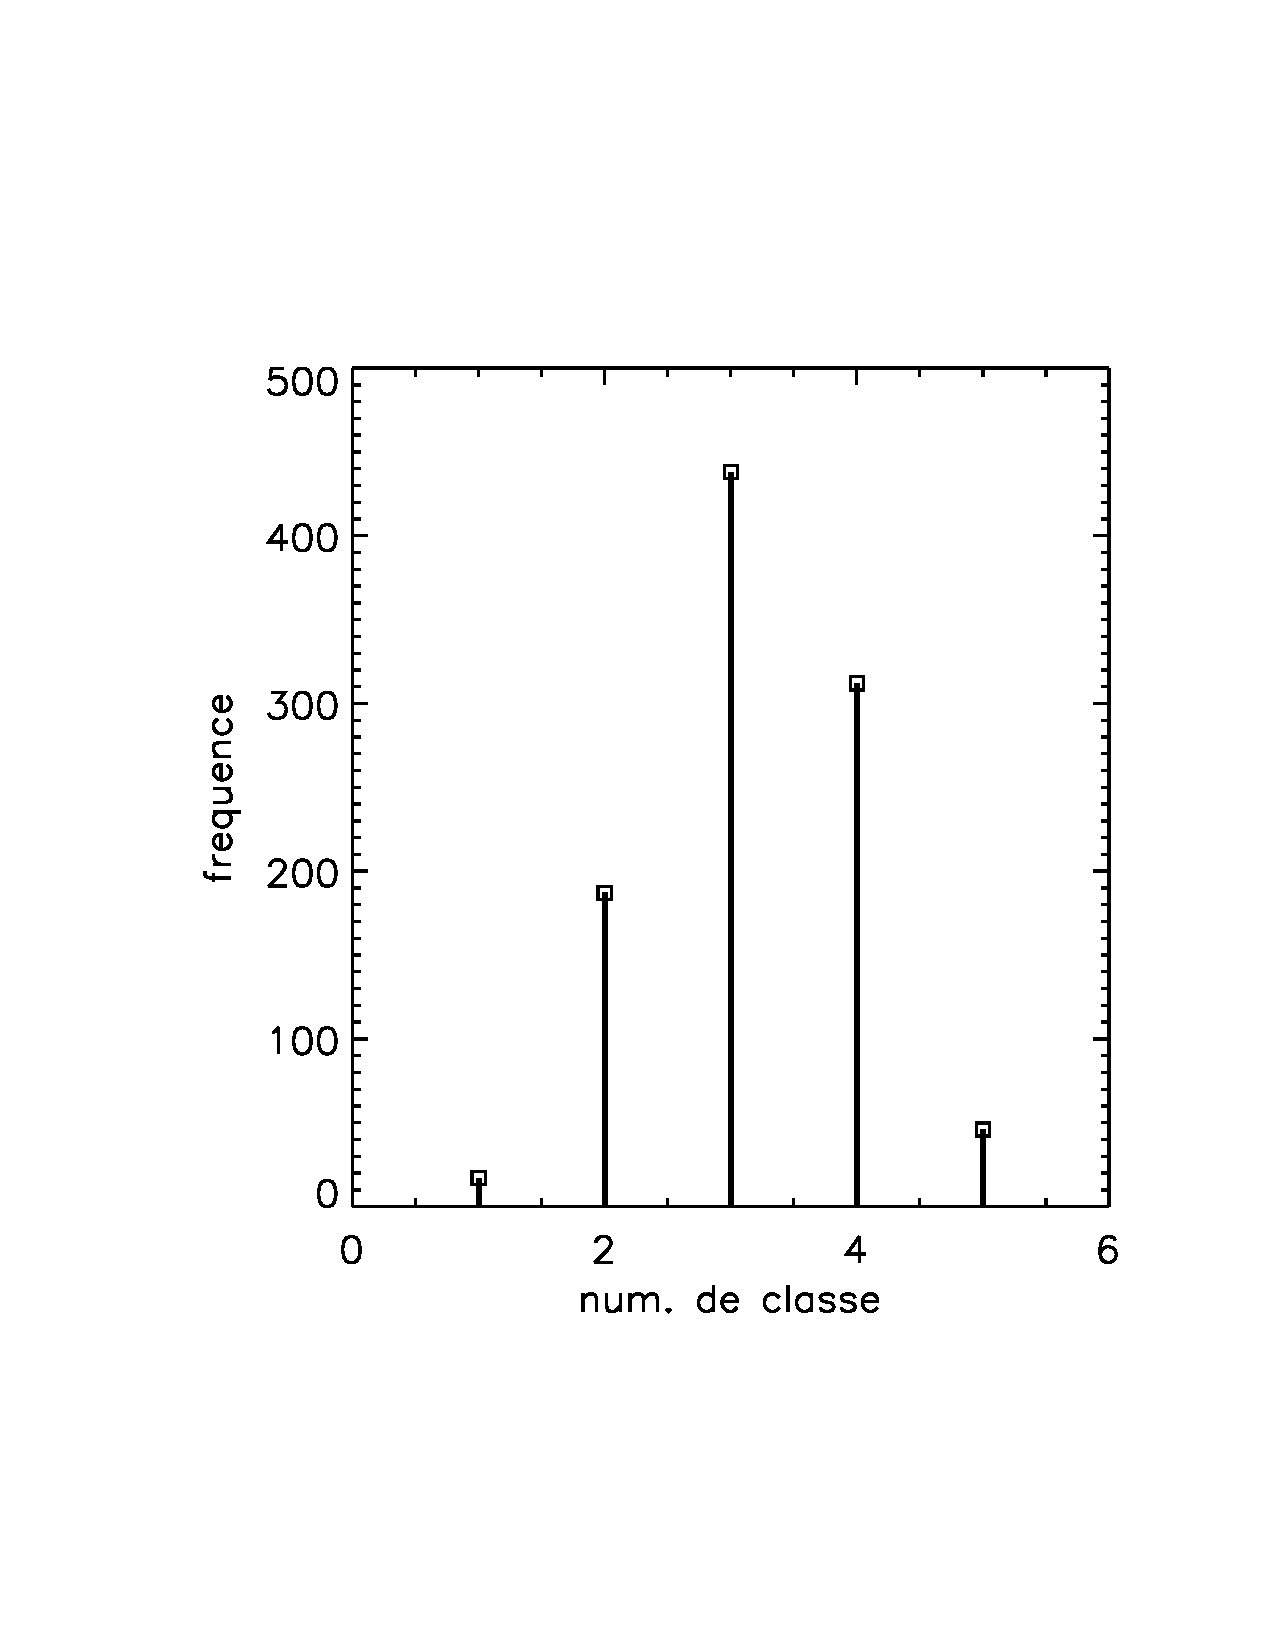
\includegraphics[width=7cm]{fig/Serie1_exe1_histogramme05classe.pdf} \hspace{5mm}
   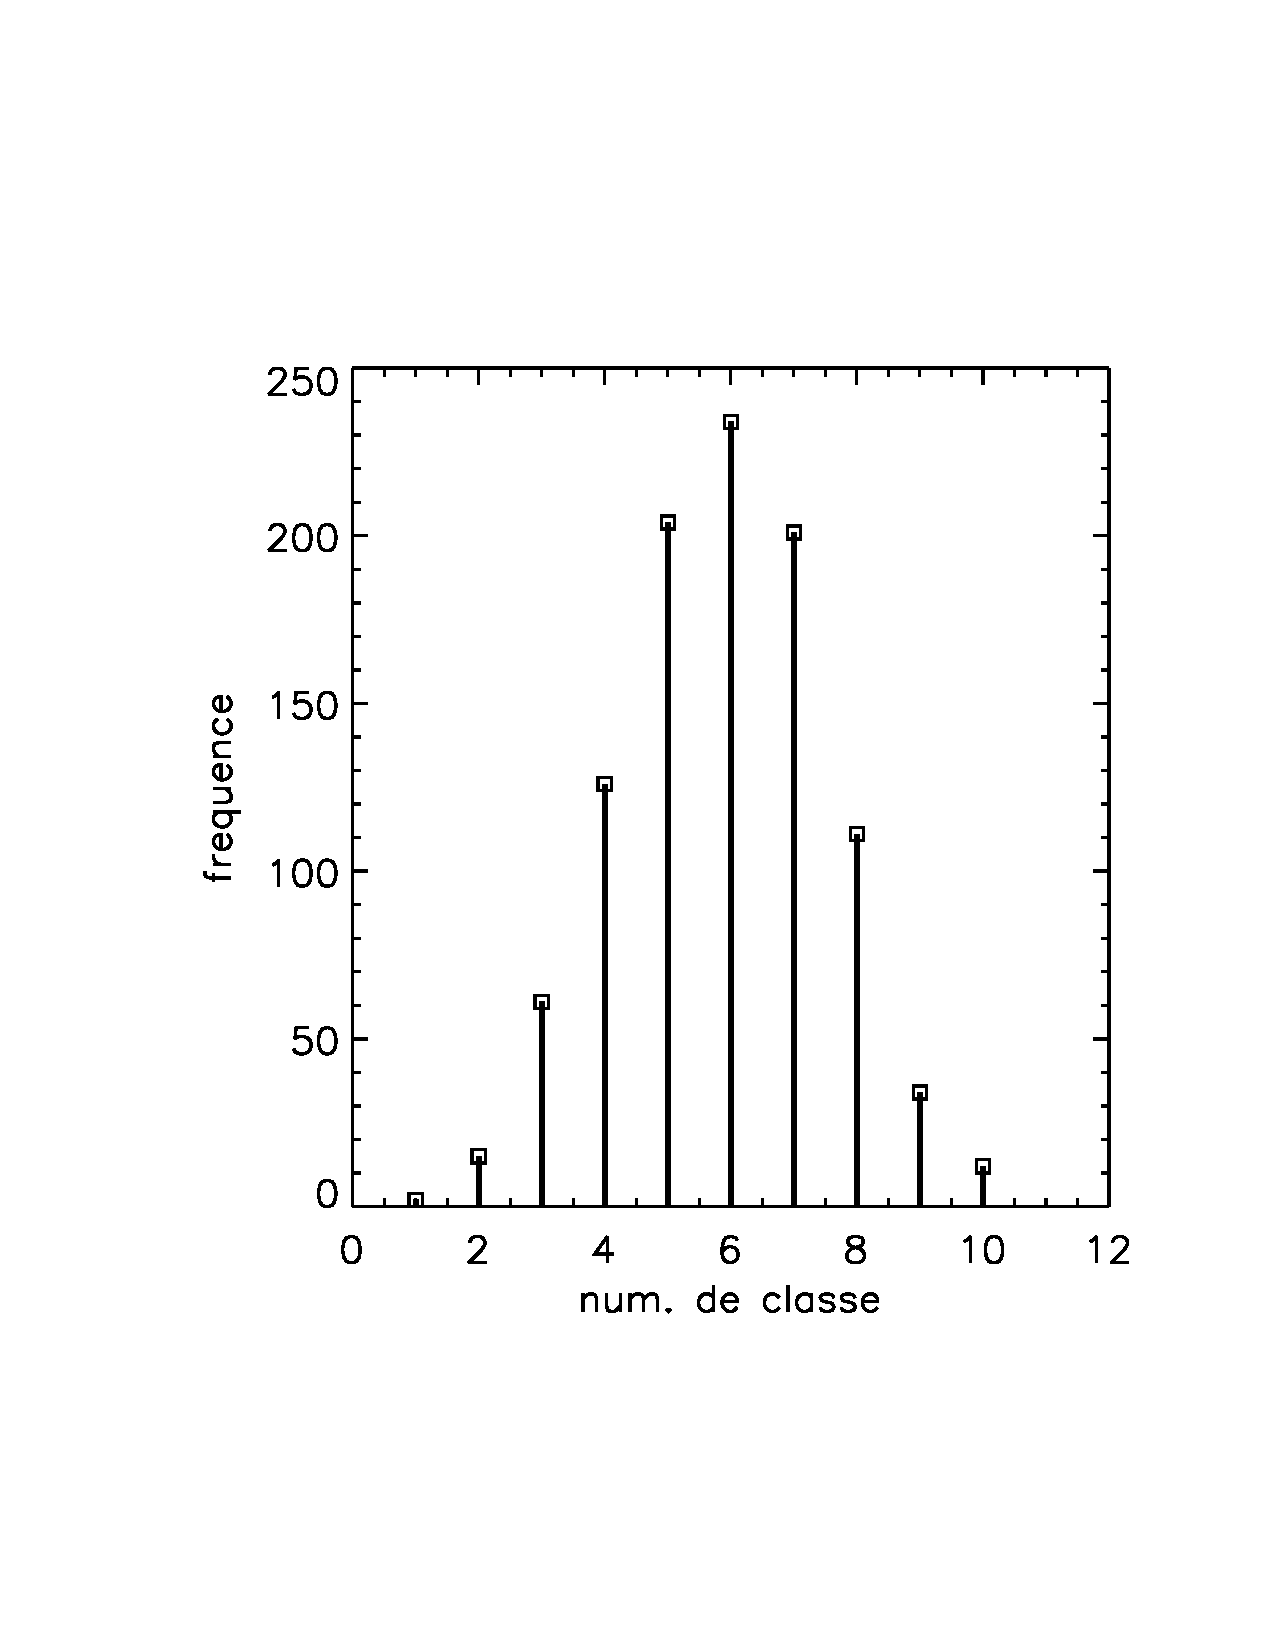
\includegraphics[width=7cm]{fig/Serie1_exe1_histogramme10classe.pdf} \\ \vspace{5mm}
   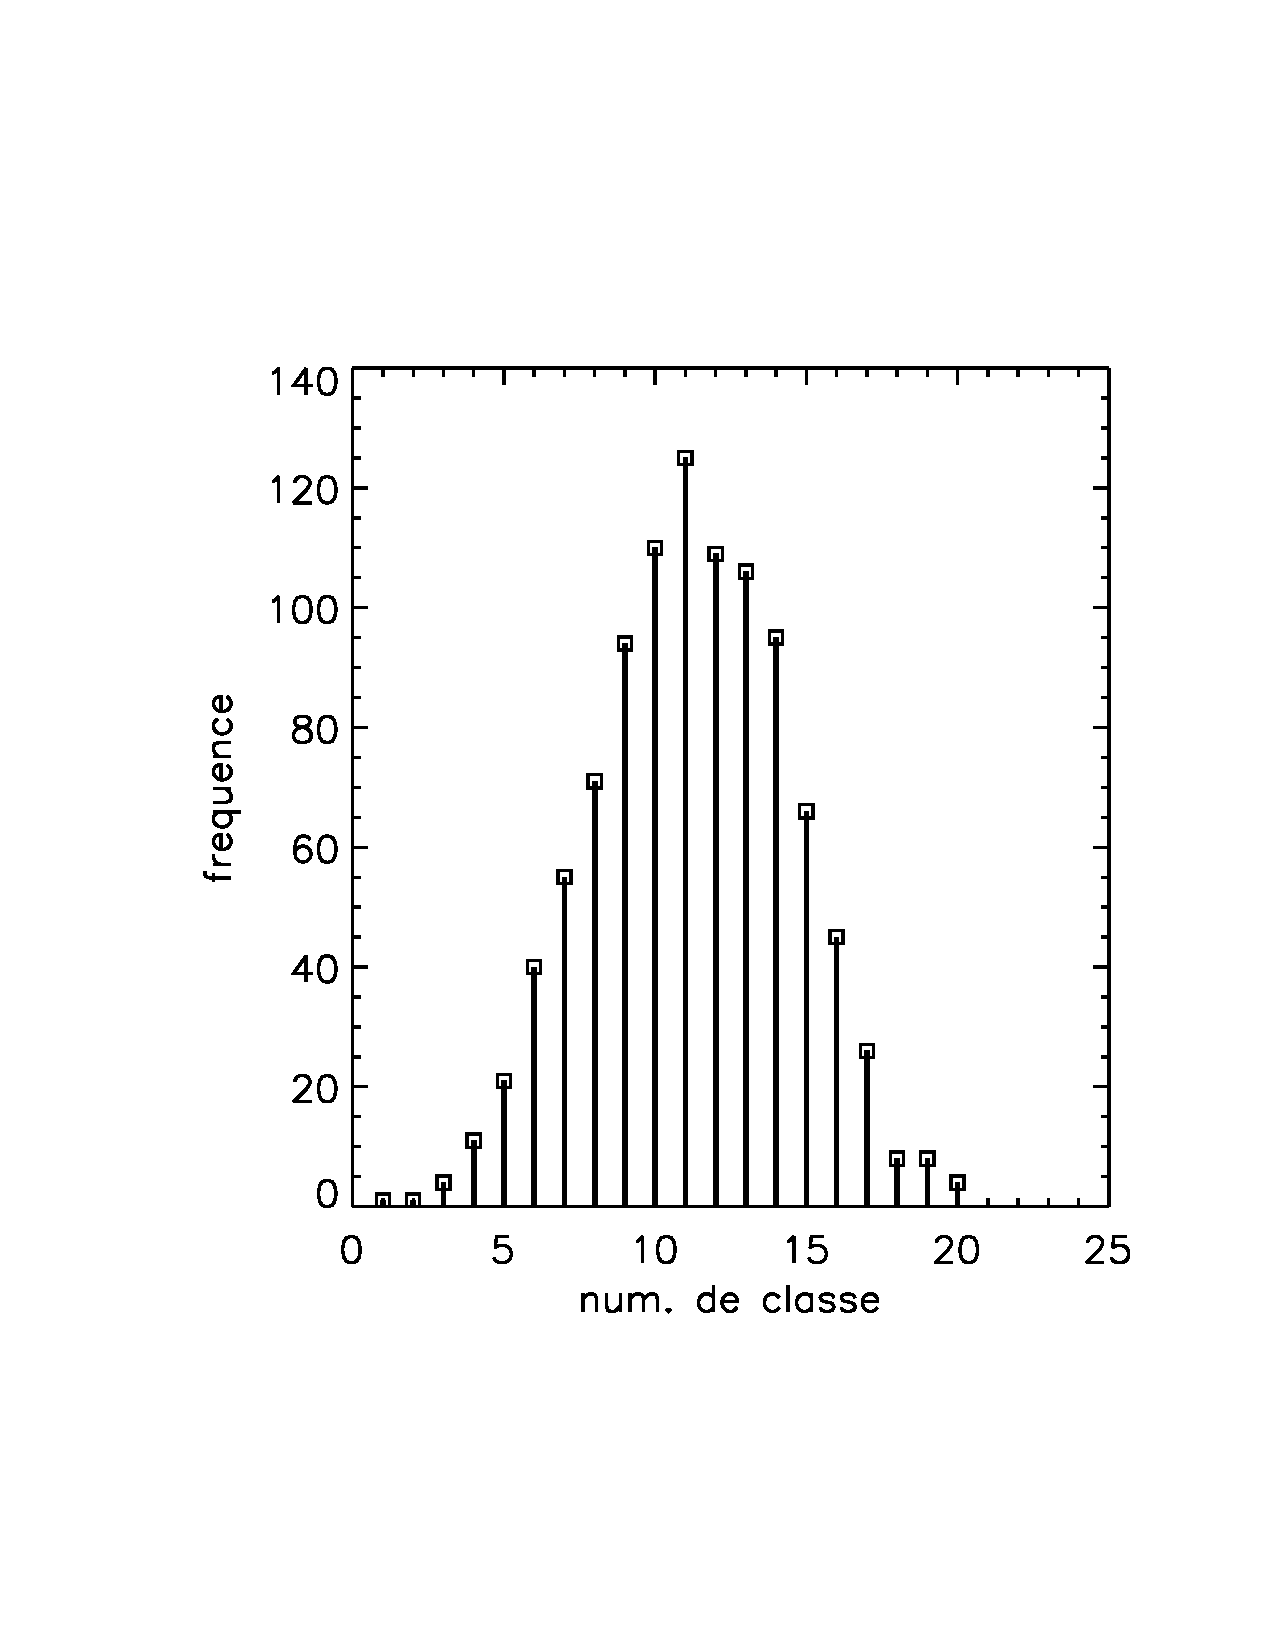
\includegraphics[width=7cm]{fig/Serie1_exe1_histogramme20classe.pdf} \hspace{5mm}
   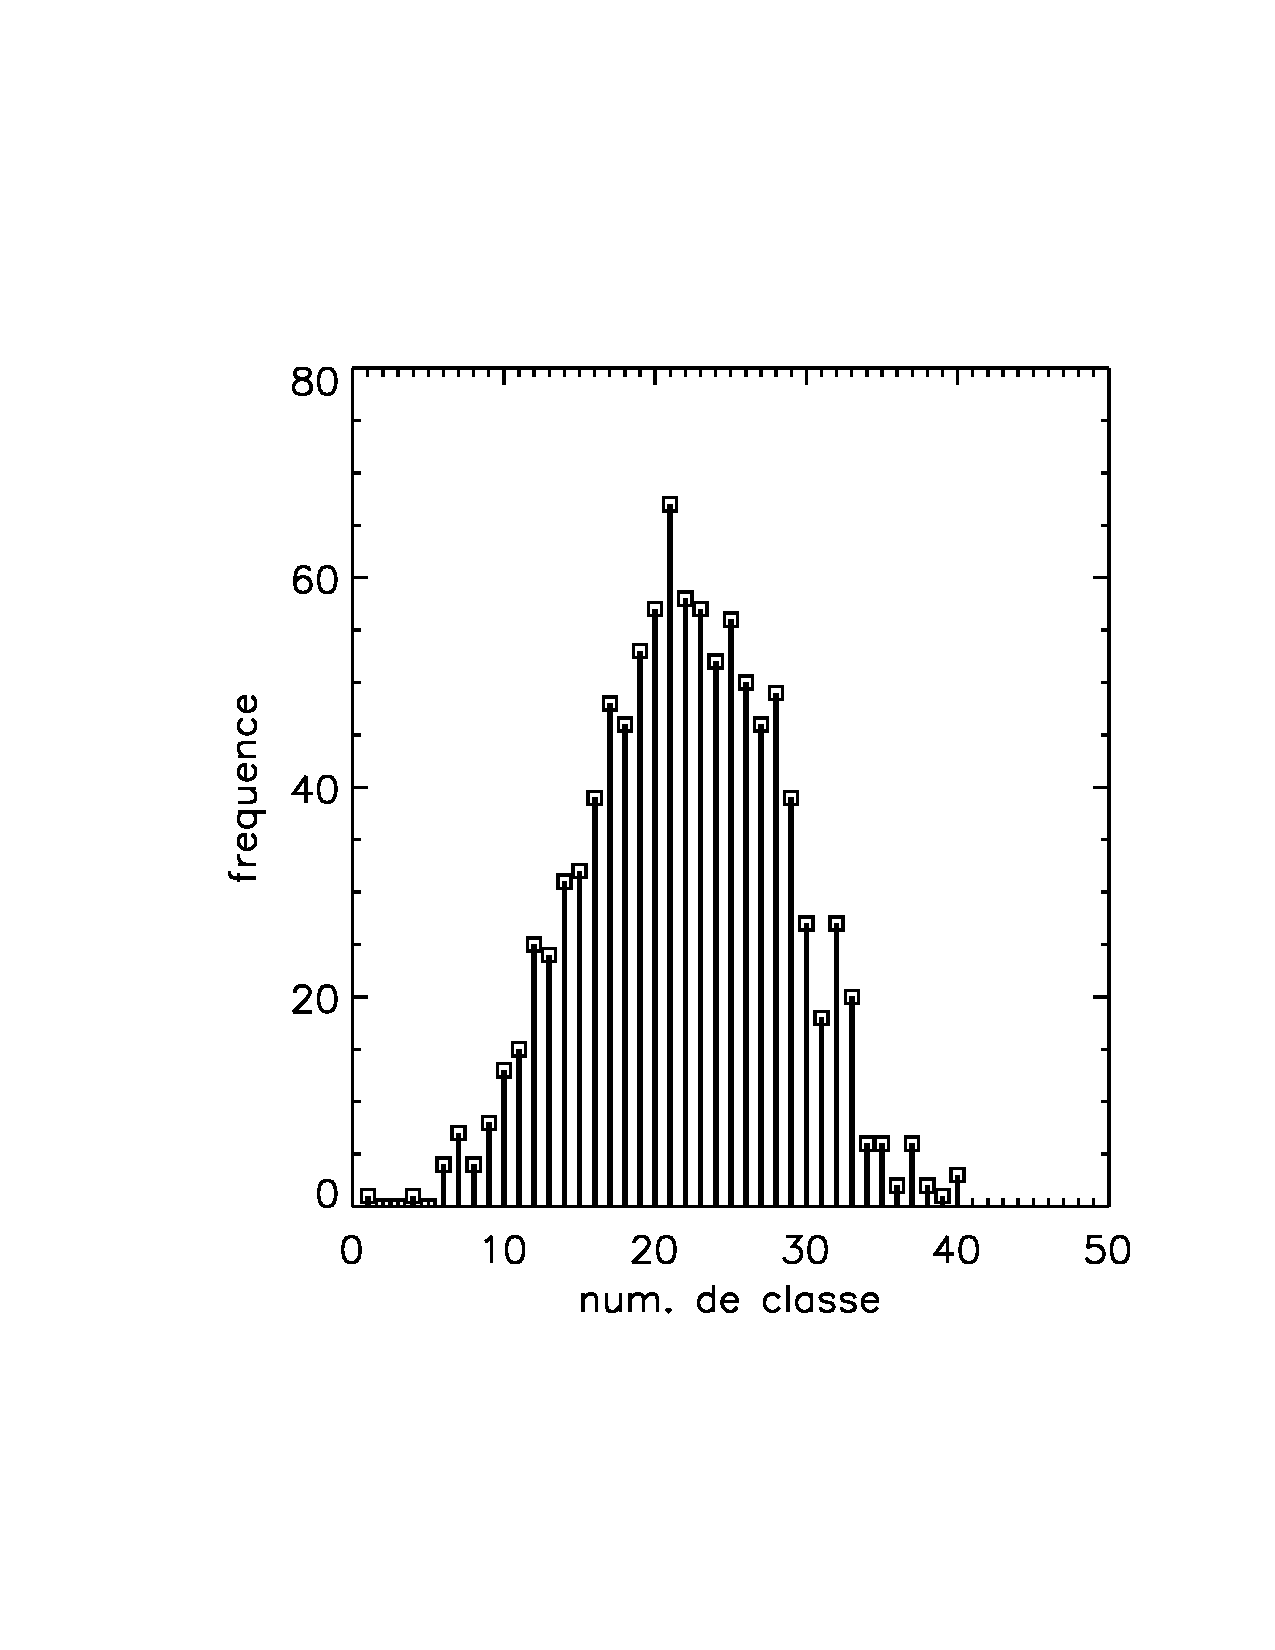
\includegraphics[width=7cm]{fig/Serie1_exe1_histogramme40classe.pdf}
   \caption{De gauche à droite et de haut en bas, histogrammes pour 5, 10, 20 et 40 classes.}
   \label{fig:hist}
\end{figure}

\newpage

\subsection*{Solution exercice 6.2 - distance de pénétration des rayons $\gamma$ dans un substrat de germanium}

\begin{enumerate}%\renewcommand{\labelitemi}{$\bullet$}
\item La moyenne est de 2236.76 mm et l'écart-type de 1649.52 mm, cependant comme il convient toujours d'arrondir au premier chiffre significatif de l'écart-type, on annoncera alors que la distance de pénétration = $2\pm 2$ m. Cela semble brutal, mais si on regarde l'histogramme des valeurs, cela a du sens (voir fig.~\ref{fig:01}) : inutile de donner la moyenne et le $\sigma$ avec plus de chiffres significatifs.
\item On trouve $\beta_1=1.09$ et $\gamma_2=0.4$
\item Une asymétrie positive indique un histogramme de valeurs avec un étirement sur la droite de la moyenne, et pour un aplatissement positif, on a un histogramme plus pointu, c'est-à-dire assez peu étalé; cependant, selon le nombre d'éléments que l'on aura dans notre échantillon (ici 50, ce qui est assez peu), et aussi selon la largeur de la classe choisie pour représenter l'échantillon, l'aplatissement (ou son inverse) ne sera pas forcément très apparent. Ces deux paramètres, $\beta_1$ et $\gamma_2$, sont de fait à prendre comme des indicateurs généraux de la structure de l'histogramme, et non pas comme des vérités absolues. Disons que plus la taille de l'échantillon sera grande, meilleur sera le pronostic donné par ces deux paramètres.
\item les tables de fréquences et les histogrammes sont donnés ci-dessous.
\begin{table}[htdp]
\caption{Classe de largeur 300, 22 intervalles --- \textbf{unités mm}}
\begin{center}
\begin{tabular}{cccccc}
\hline
num. & classe & valeur & occurrence & fréquence & fréquence\\
inter. &  & centrale & dans la classe & d'occurrence \% & cumulée \%\\\hline
 1 & $  41 \rightarrow  341$ &  191 & 1 &  2 &   2\\
 2 & $ 341 \rightarrow  641$ &  491 & 5 & 10 &  12\\
 3 & $ 641 \rightarrow  941$ &  791 & 4 &  8 &  20\\
 4 & $ 941 \rightarrow 1241$ & 1091 & 6 & 12 &  32\\
 5 & $1241 \rightarrow 1541$ & 1391 & 4 &  8 &  40\\
 6 & $1541 \rightarrow 1841$ & 1691 & 7 & 14 &  54\\
 7 & $1841 \rightarrow 2141$ & 1991 & 5 & 10 &  64\\
 8 & $2141 \rightarrow 2441$ & 2291 & 4 &  8 &  72\\
 9 & $2441 \rightarrow 2741$ & 2591 & 0 &  0 &  72\\
10 & $2741 \rightarrow 3041$ & 2891 & 1 &  2 &  74\\
11 & $3041 \rightarrow 3341$ & 3191 & 1 &  2 &  76\\
12 & $3341 \rightarrow 3641$ & 3491 & 1 &  2 &  78\\
13 & $3641 \rightarrow 3941$ & 3791 & 2 &  4 &  82\\
14 & $3941 \rightarrow 4241$ & 4091 & 3 &  6 &  88\\
15 & $4241 \rightarrow 4541$ & 4391 & 1 &  2 &  90\\
16 & $4541 \rightarrow 4841$ & 4691 & 0 &  0 &  90\\
17 & $4841 \rightarrow 5141$ & 4991 & 2 &  4 &  94\\
18 & $5141 \rightarrow 5441$ & 5291 & 0 &  0 &  94\\
19 & $5441 \rightarrow 5741$ & 5591 & 0 &  0 &  94\\
20 & $5741 \rightarrow 6041$ & 5891 & 0 &  0 &  94\\
21 & $6041 \rightarrow 6341$ & 6191 & 0 &  0 &  94\\
22 & $6341 \rightarrow 6641$ & 6491 & 3 &  6 &  100\\
\hline
\end{tabular}
\end{center}
\label{tab:01}
\end{table}
\vspace{1.5cm}

\begin{table}[htdp]
\caption{Classe de largeur 1200, 6 intervalles --- \textbf{unités mm}}
\begin{center}
\begin{tabular}{cccccc}
\hline
num. & classe & valeur & occurrence & fréquence & fréquence\\
inter. &  & centrale & dans la classe & d'occurrence \% & cumulée \%\\\hline
 1 & $  41 \rightarrow 1241$ &  641 & 16 & 32 &  32\\
 2 & $1241 \rightarrow 2441$ & 1841 & 20 & 40 &  72\\
 3 & $2441 \rightarrow 3641$ & 3041 &  3 &  6 &  78\\
 4 & $3641 \rightarrow 4841$ & 4241 &  6 & 12 &  90\\
 5 & $4841 \rightarrow 6041$ & 5441 &  2 &  4 &  94\\
 6 & $6041 \rightarrow 7241$ & 6641 &  3 &  6 & 100\\
\hline
\end{tabular}
\end{center}
\label{tab:02}
\end{table}

\begin{table}[htdp]
\caption{Classe de largeur 3000, 3 intervalles --- \textbf{unités mm}}
\begin{center}
\begin{tabular}{cccccc}
\hline
num. & classe & valeur & occurrence & fréquence & fréquence\\
inter. &  & centrale & dans la classe & d'occurrence \% & cumulée \%\\\hline
 1 & $  41 \rightarrow 3041$ & 1541 & 37 & 74 &  74\\
 2 & $3041 \rightarrow 6041$ & 4541 & 10 & 20 &  94\\
 3 & $6041 \rightarrow 9041$ & 7541 & 3 &  6 & 100\\
\hline
\end{tabular}
\end{center}
\label{tab:03}
\end{table}

\newpage
On remarquera que les classes sont incrémentées à partir de la valeur minimale de l'échantillon, à savoir ici 41 mm, et non à partir de 0.
\begin{figure}[htbp] %  figure placement: here, top, bottom, or page
   \centering
   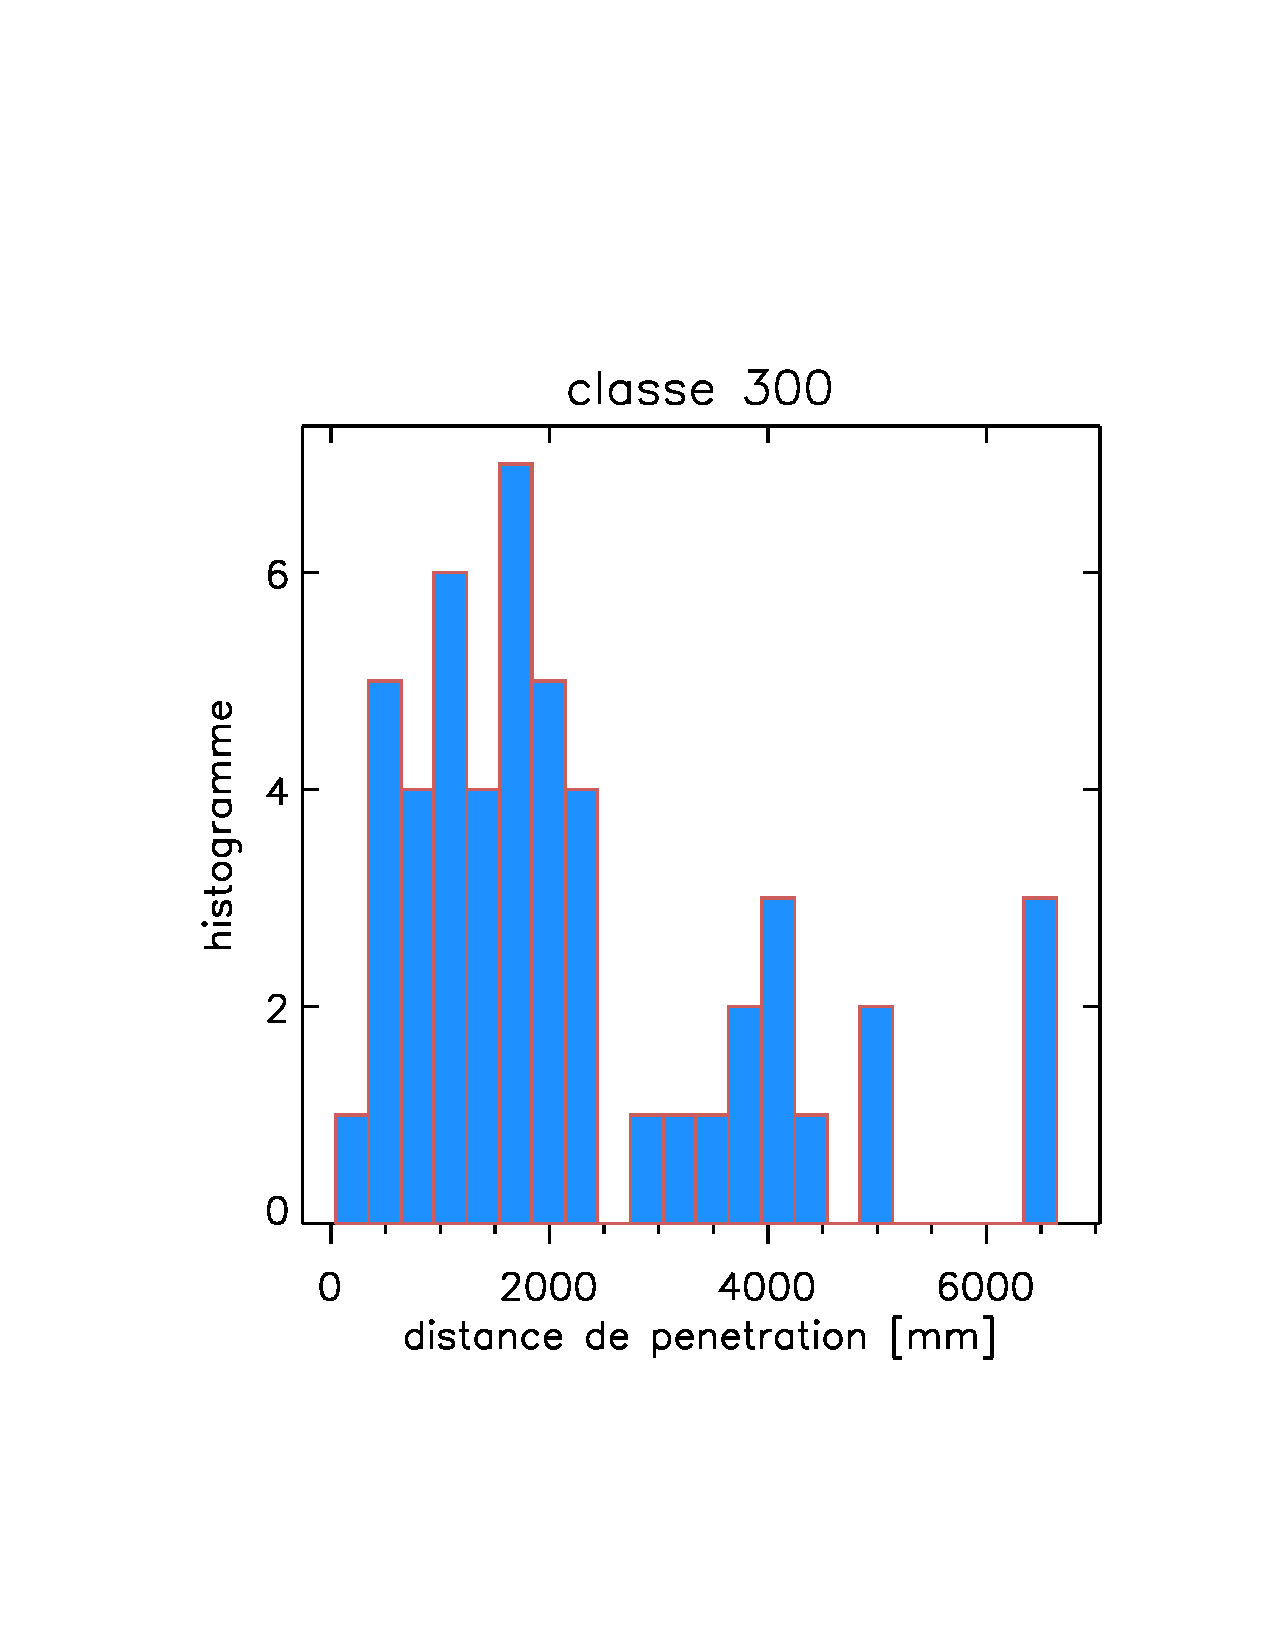
\includegraphics[height=56mm]{fig/Serie1_exe2_histogramClasse0300.pdf}
   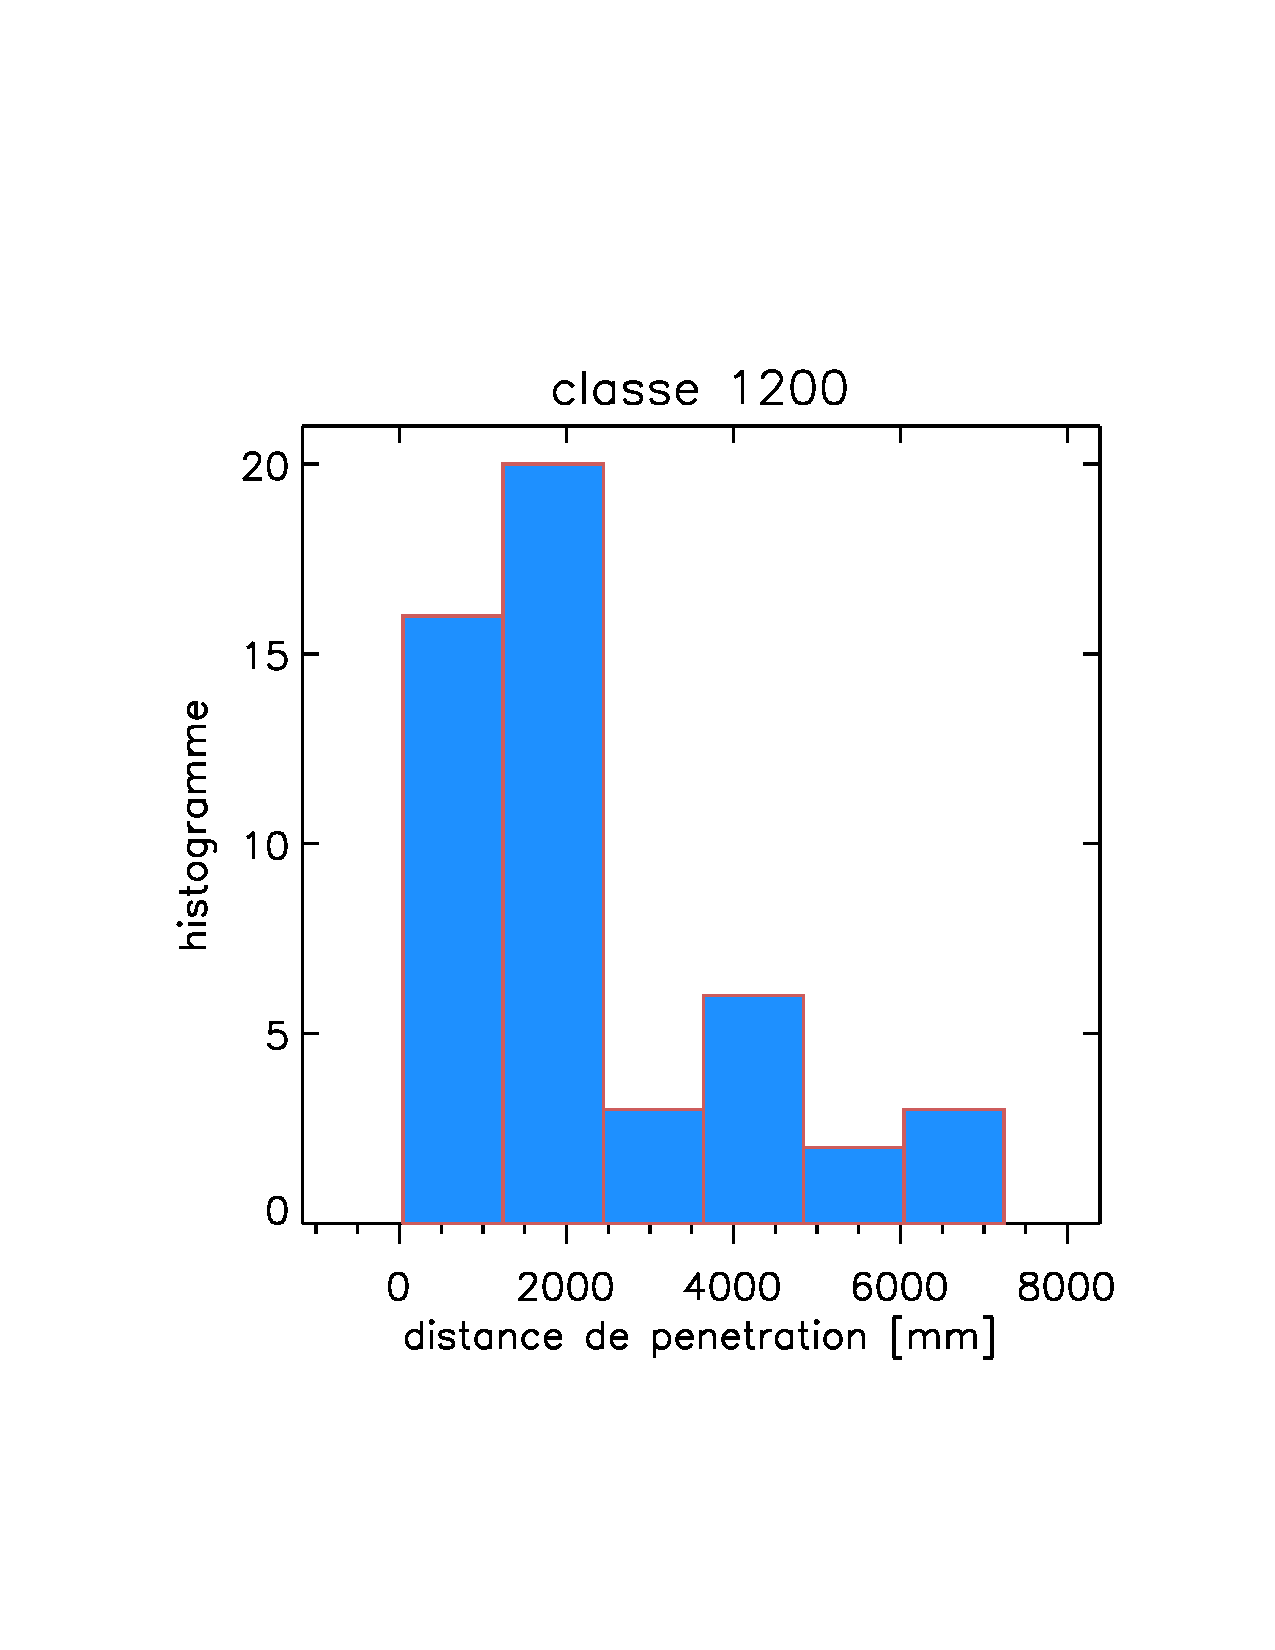
\includegraphics[height=56mm]{fig/Serie1_exe2_histogramClasse1200.pdf}
   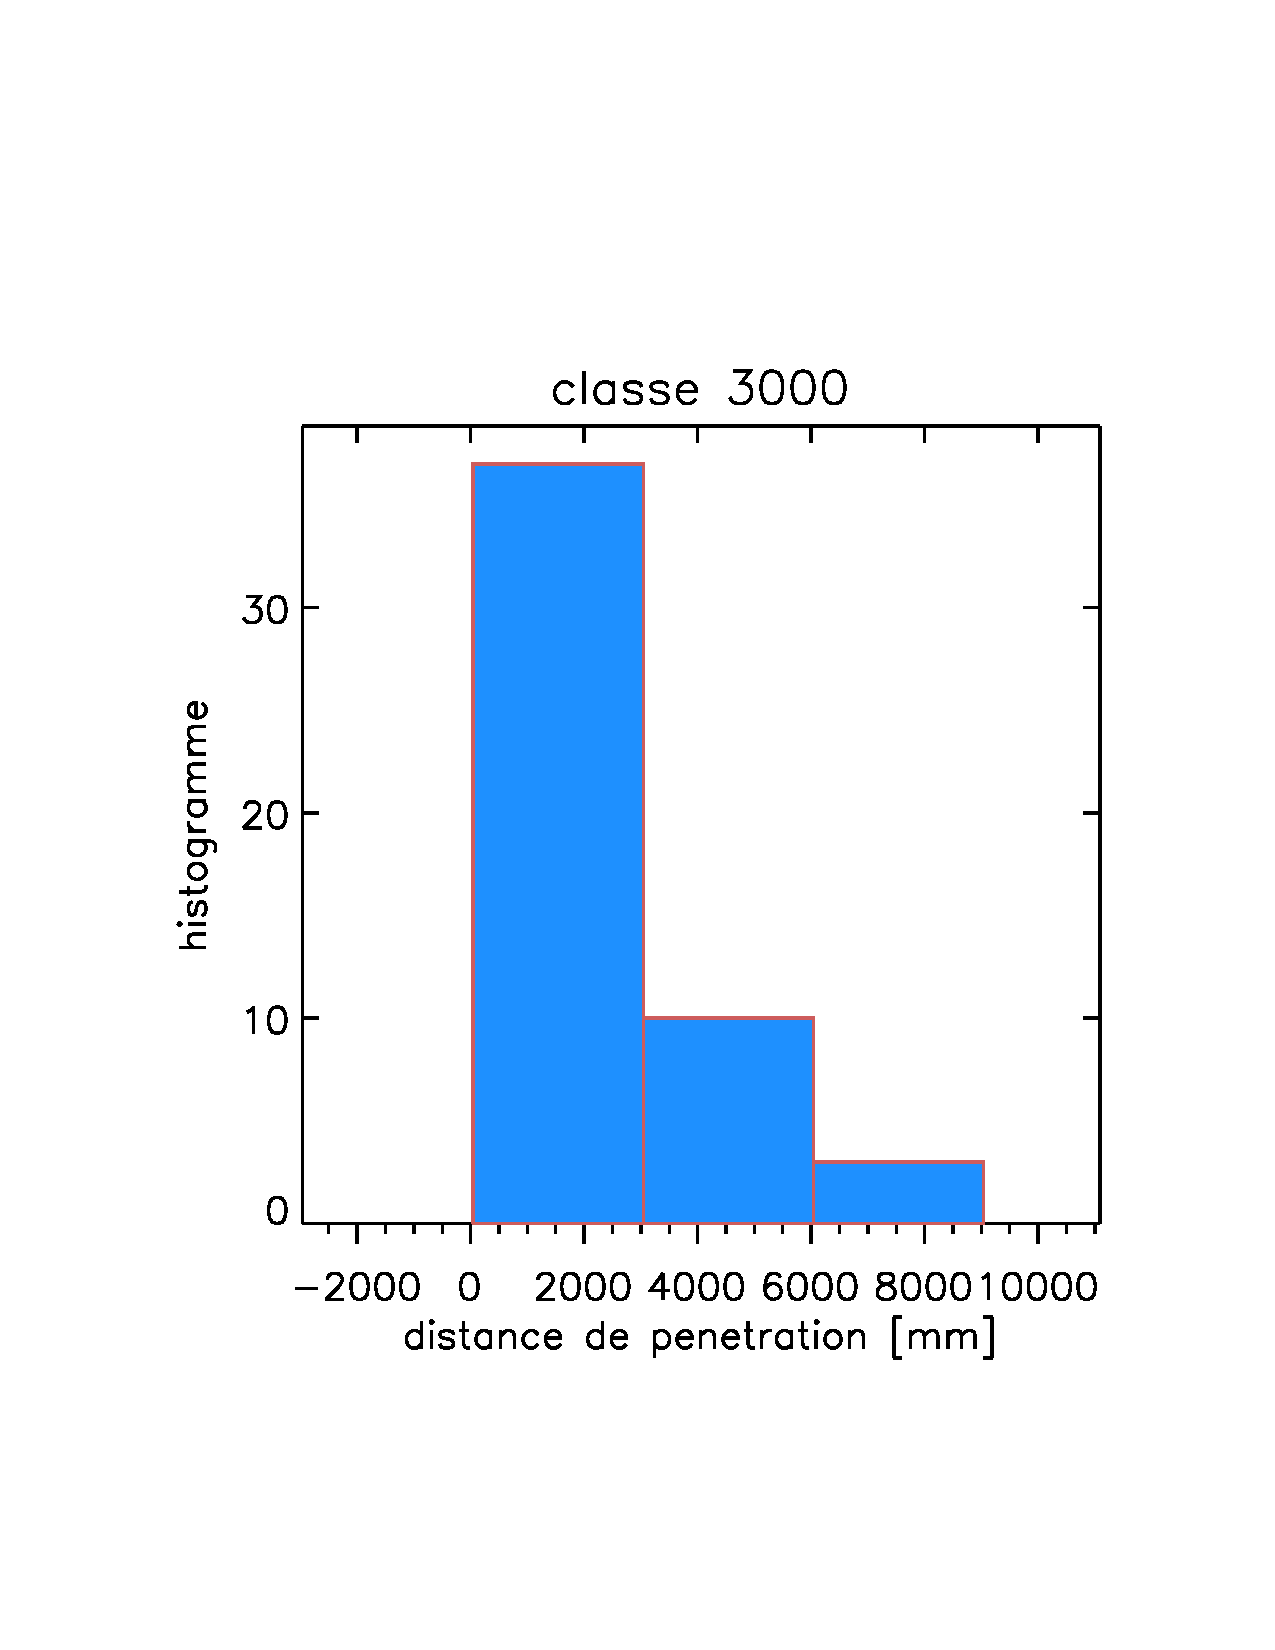
\includegraphics[height=56mm]{fig/Serie1_exe2_histogramClasse3000.pdf}
   \caption{Histogrammes associés aux classes de largeur 300, 1200 et 3000.}
   \label{fig:02}
\end{figure}
%\newpage
\item on applique la théorie du cours :
\begin{gather}
\langle x \rangle \approx \frac{1}{N_{ech}}\sum\limits_{k=1}^{N_c} x_k H_k\\
\langle x^2 \rangle \approx \frac{1}{N_{ech}}\sum\limits_{k=1}^{N_c} x_k^2 H_k\\
\sigma_x=\sqrt{\langle x^2 \rangle-\langle x \rangle^2}
\end{gather}
où $N_{ech}$ est le nombre d'échantillons (ici 50), $N_c$ le nombre d'intervalles pour une classe donnée, soit ici 3, 6 et 22 (pour les classes 3000, 1200 et 300), $x_k$ est la valeur de $\Delta$ au centre de l'intervalle $k$, et $H_k$ est la valeur de l'histogramme associé à la valeur $x_k$. Pour les trois classes, on trouve les résultats suivants :
\begin{center}
\begin{tabular}{rcccc}
 & classe & classe & classe & valeur\\
\textbf{unités : mm} & 300 & 1200 & 3000 & exacte\\\hline
valeur moyenne $\langle x \rangle$ & 2243 & 2249 & 2501 & 2236.76 \\
sans corr. Sheppard $\sigma_x$ & 1631 & 1724 & 1743 & 1649.52\\
err. $\sigma_x$ & -18 & 75 & 94 & ---\\
avec corr. Sheppard $\sigma_x'$ & 1629 & 1689 & 1513 & 1649.52\\
err $\sigma_x'$ & -20 & 39 & -137 & ---\\
\hline
\end{tabular}
\end{center}
on remarquera que la correction de Sheppard sur la variance (ici exprimée en écart-type) n'a pas un effet extraordinaire pour notre échantillon, et en fait, ce n'est pas très étonnant, car cette correction ne s'applique que si l'échantillon est de statistique gaussienne. Ce qui n'est clairement pas le cas ici : on le sait déjà par les valeurs des paramètres $\beta_1$ et de $\gamma_2$, et surtout par inspection visuelle des histogrammes, qui ont une allure plutôt du type distribution de Poisson (voir cours).
\item examinons l'histogramme pour la classe 1200 (fig. \ref{fig:02}, centre), ainsi que le tableau des fréquences (table \ref{tab:02}). On sait que notre échantillon de distances de pénétration a 50 valeurs. La valeur médiane de la distance est définie comme la valeur de $\Delta$ qui sépare l'histogramme en deux parties de même somme, c'est-à-dire que le nombre de valeurs de $\Delta\le$ médiane est égale au nombre de valeurs de $\Delta\ge$ médiane. En d'autres termes, la médiane est la valeur telle que la fréquence cumulée est de 50 \%.

Si on examine la fréquence cumulée (colonne de droite), on voit que la valeur médiane de $\Delta$ doit se trouver quelque part entre les valeurs de $\Delta$ associées au premier et au deuxième intervalle de classe. Dans l'histogramme, la valeur de $\Delta$ associée à l'intervalle $k$ est le milieu de l'intervalle, donc $(1241+41)/2=641$ mm pour la première valeur et $(1241+2441)/2=1841$ mm pour la seconde. Nous allons interpoler entre ces deux valeurs. Les éléments (pente, ordonnée à l'origine) de la droite qui passe par les deux points $(\text{fréq. cumul.},\Delta)$ (32,641) et (72,1841) sont donnés par
$$
m=\frac{1841-641}{72-32}=30\ \ \ \ \ \ p=1841-m\cdot72=-319
$$
la valeur interpolée de la médiane est donc égale à $30\cdot50-319=1181$ mm.

Quant au mode, c'est très simple, c'est la valeur la plus fréquente (pour cette valeur de la classe et uniquement pour cette valeur), soit 1841 mm. Et le mode serait 1691 mm et 1541 mm pour les deux autres classes. On voit donc bien avec cet exercice que la manière de choisir la classe de l'histogramme a une énorme influence sur le calcul des caractéristiques statistiques d'un échantillon, et qu'il faut donc choisir la classe avec soin. Clairement, dans notre cas, la classe 1200 mm est encore acceptable, mais pas la classe 3000 mm.
\end{enumerate}

\subsection*{Solution exercice 6.3 - pression atmosphérique martienne, Gusev crater}

\textbf{Q1~:} il faut 102 (ou moins) classes pour obtenir au moins 10 mesures dans la classe la plus peuplée, mais en fait, avec 102 classes, l'histogramme est assez chahuté et assez peu représentatif; il vaudrait mieux prendre moins de classes.

\textbf{Q2, Q3~:} Si nous conservons néanmoins 102 classes, alors les fréquences cumulées, données par la somme des fréquences dans toutes les classes inférieures à la classe $i$, selon
$$
F_k=\sum\limits_{j=1}^{k}\,f_j
$$
sont données ci-dessous, et l'histogramme cumulé est donné en fig.~\ref{fig:ch}.
\begin{center}
\scriptsize
\begin{tabular}{cccccccccccccccccccc}
$k$ & $F_k$ & $k$ & $F_k$ & $k$ & $F_k$ & $k$ & $F_k$ & $k$ & $F_k$ & $k$ & $F_k$ & $k$ & $F_k$ & $k$ & $F_k$ & $k$ & $F_k$ & $k$ & $F_k$ \\\hline
 1 & 1 & 11 &  8 & 21 & 25 & 31 &  50 & 41 & 106 & 51 & 167 & 61 & 218 & 71 & 256 & 81 & 268 &  91 & 273\\
 2 & 1 & 12 & 11 & 22 & 30 & 32 &  55 & 42 & 111 & 52 & 176 & 62 & 226 & 72 & 262 & 82 & 269 &  92 & 273\\
 3 & 2 & 13 & 12 & 23 & 31 & 33 &  61 & 43 & 119 & 53 & 180 & 63 & 231 & 73 & 263 & 83 & 269 &  93 & 273\\
 4 & 2 & 14 & 14 & 24 & 33 & 34 &  66 & 44 & 129 & 54 & 186 & 64 & 234 & 74 & 264 & 84 & 270 &  94 & 273\\
 5 & 4 & 15 & 14 & 25 & 35 & 35 &  72 & 45 & 135 & 55 & 193 & 65 & 237 & 75 & 265 & 85 & 272 &  95 & 274\\
 6 & 4 & 16 & 16 & 26 & 37 & 36 &  76 & 46 & 138 & 56 & 198 & 66 & 244 & 76 & 266 & 86 & 272 &  96 & 274\\
 7 & 5 & 17 & 17 & 27 & 37 & 37 &  82 & 47 & 146 & 57 & 203 & 67 & 247 & 77 & 266 & 87 & 273 &  97 & 274\\
 8 & 6 & 18 & 17 & 28 & 37 & 38 &  88 & 48 & 150 & 58 & 208 & 68 & 250 & 78 & 266 & 88 & 273 &  98 & 274\\
 9 & 6 & 19 & 20 & 29 & 41 & 39 &  94 & 49 & 152 & 59 & 210 & 69 & 250 & 79 & 266 & 89 & 273 &  99 & 274\\
10 & 7 & 20 & 22 & 30 & 45 & 40 & 100 & 50 & 162 & 60 & 215 & 70 & 254 & 80 & 267 & 90 & 273 & 100 & 274\\
101 & 274 \\
102 & 275 \\\hline
\end{tabular}
\normalsize
\end{center}

\begin{wrapfigure}[7]{l}[10pt]{7cm}
   \centering
   \vspace{-5mm}
   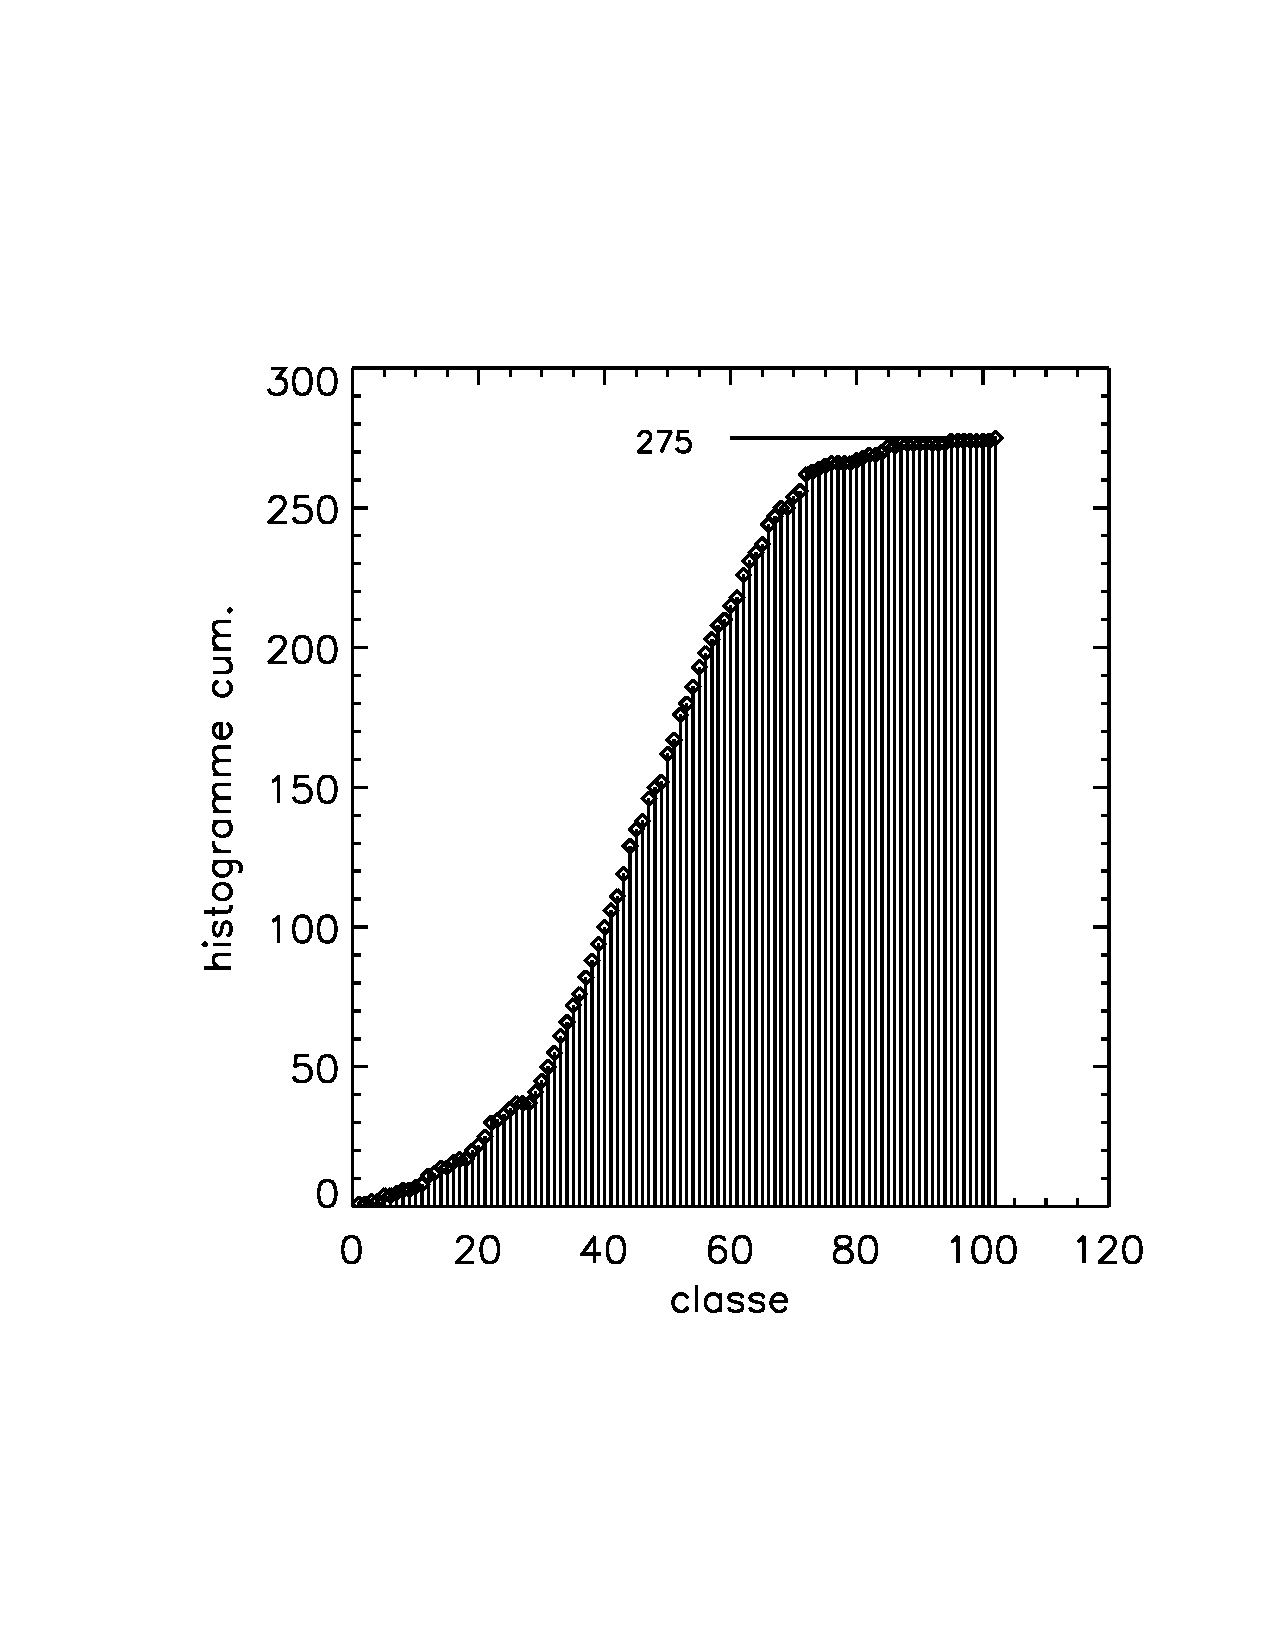
\includegraphics[width=7cm]{fig/Serie1_exe3_histCumulated.pdf}
   \caption{Histogramme cumulé.}
   \label{fig:ch}
\end{wrapfigure}
\textbf{Q4~:} Il suffit de compter le nombre de mesures qui se trouvent égales ou supérieures à 890 Pa. On trouve que durant 174 sols sur 275 (1 sol = 1 jour martien = 24 h 40 min terrestres), l'eau aurait pu être liquide au fond du cratère Gusev. Les probabilités d'obtenir des conditions favorables à la vie sont donc de $174/275=63\%$.

%----------
\section{Solutions des exercices du chapitre 7}
%----------

\subsection*{Solution de l'exercice 7.1}

\paragraph{Population.} En jetant deux dés, les résultats que l'on peut obtenir vont de 2 à 12. La population, qui est l'ensemble des résultats possibles, est donc
$$
\Omega=[2,3,4,5,6,7,8,9,10,11,12]
$$
et la dimension de cette population est de 11 éléments.

\paragraph{Probabilité de chaque valeur.} Examinons quelles combinaison de jet de dés peuvent conduire à chacune des valeurs de la population. On a
\begin{center}
\begin{tabular}{llll}
i & somme des & combinaisons possibles & nombre de combi- \\
& dés, $v_i$ & pour obtenir $v_i$ & naisons $C(v_i)$\\ \hline
1 & 2 & (1,1) & 1 \\
2 & 3 & (1,2) (2,1) & 2 \\
3 & 4 & (1,3) (2,2) (3,1) & 3 \\
4 & 5 & (1,4) (2,3) (3,2) (4,1) & 4 \\
5 & 6 & (1,5) (2,4) (3,3) (4,2) (5,1) & 5 \\
6 & 7 & (1,6) (2,5) (3,4) (4,3) (5,2) (6,1) & 6\\
7 & 8 & (2,6) (3,5) (4,4) (5,3) (6,2) & 5 \\
8 & 9 & (3,6) (4,5) (5,4) (6,3) & 4 \\
9 & 10 & (4,6) (5,5) (6,4) & 3 \\
10 & 11 & (5,6) (6,5) & 2 \\
11 & 12 & (6,6) & 1 \\\hline
& & & $\sum_{i=1}^{11}C(v_i)=36$
\end{tabular}
\end{center}

\begin{wrapfigure}[6]{l}[0pt]{6.0cm}
	\centering
	\vspace{-5mm}
	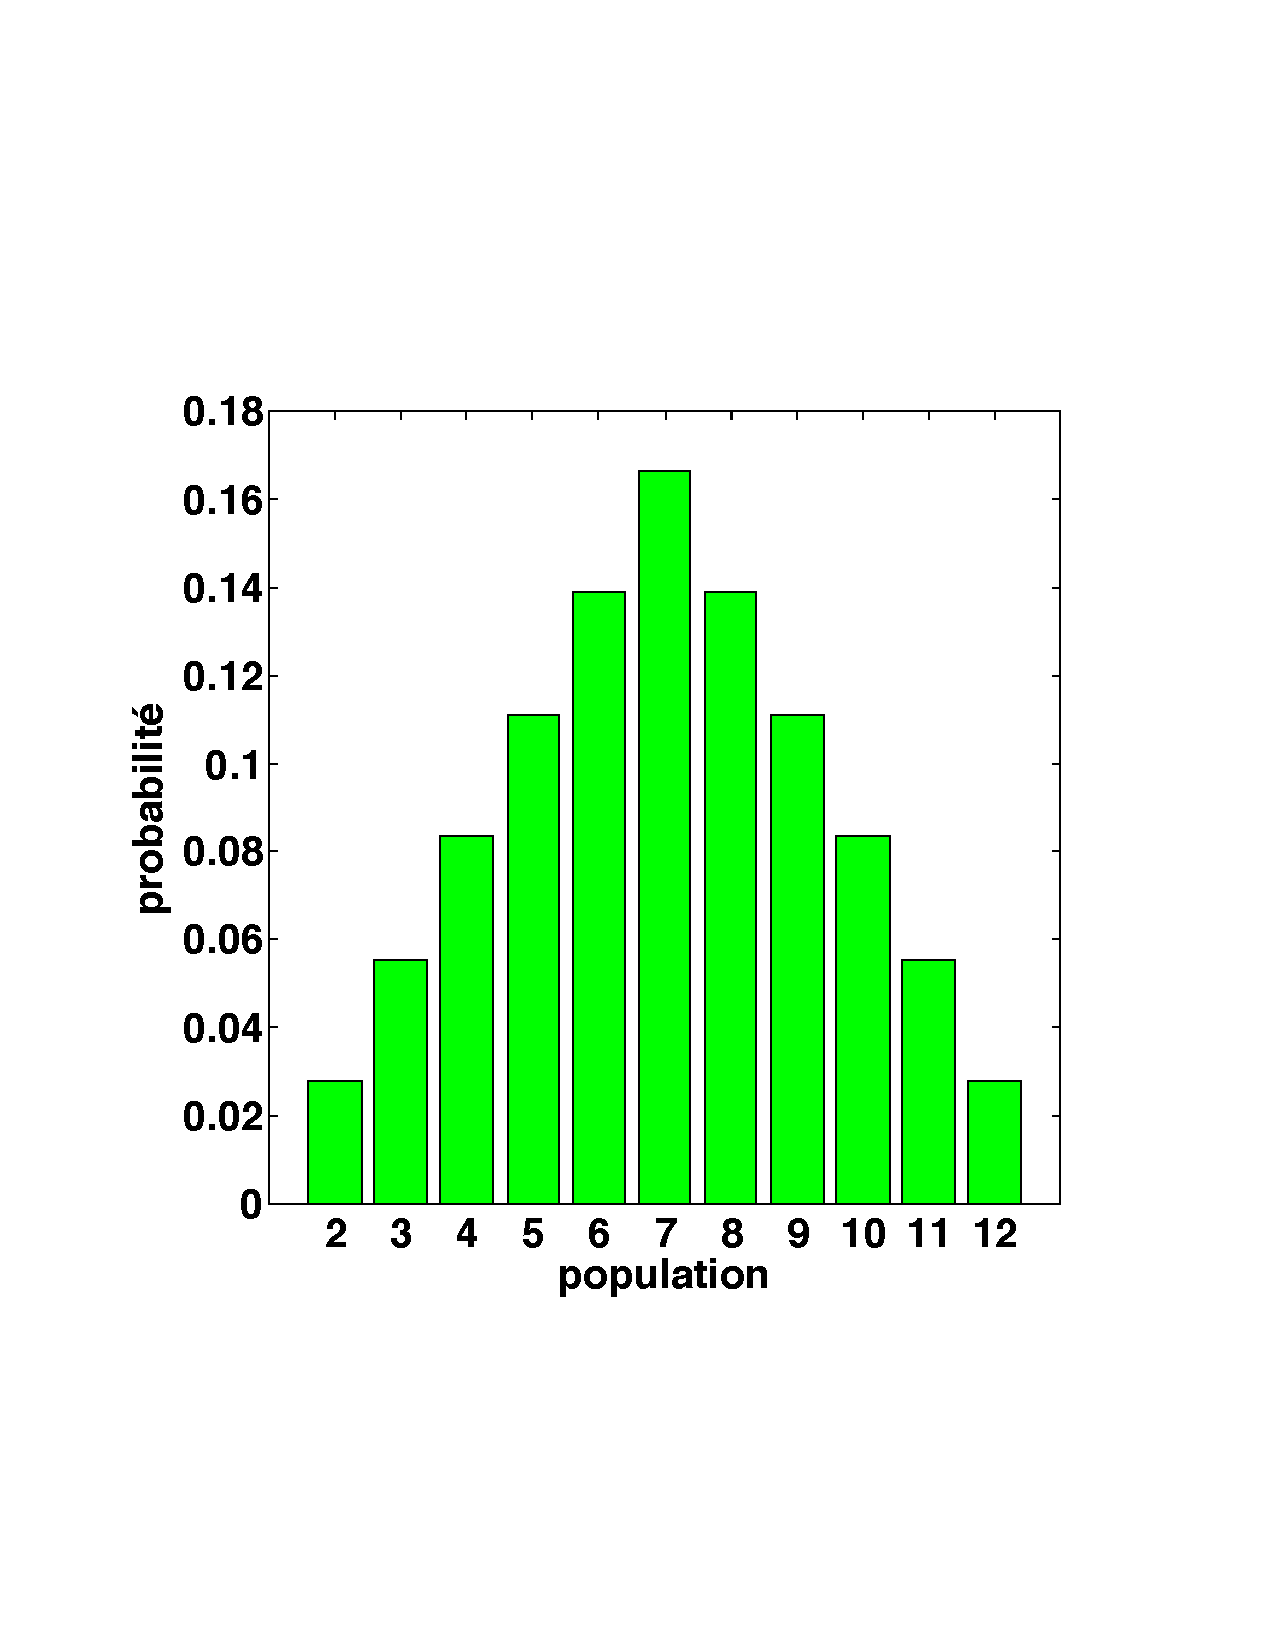
\includegraphics[width=6.0cm]{assets/figures/Serie2_exe01fig1.pdf}
	\caption{Jet de 2 dés.}
	\label{fig:exe1fig1}
\end{wrapfigure}
La probabilité d'une des valeurs $v_i$ de la population est donc donnée par le nombre de combinaisons engendrant cette valeur, $C(v_i)$, divisée par le nombre total de combinaisons possibles, soit $p(v_i)=C(v_i)/\sum_{i=1}^{11}C(v_i)=C(v_i)/36$, et il vient\vspace{1mm}\\
\begin{tabular}{c|ccccccccccc}\hline
$v_i$ & 2 & 3 & 4 & 5 & 6 & 7 \\
$p_i$ & 1/36 & 2/36 & 3/36 & 4/36 & 5/36 & 6/36 \\
\%    & 2.78 & 5.56 & 8.33 & 11.11 & 13.89 & 16.67 \\\hline\hline
$v_i$ & 8 & 9 & 10 & 11 & 12 \\
$p_i$ & 5/36 & 4/36 & 3/36 & 2/36 & 1/36 \\
\%    & 13.89 & 11.11 & 8.33 & 5.56 & 2.78 \\\hline
\end{tabular}

\paragraph{Modes, médiane, moyenne.} Ici, le mode est 7. La médiane, qui sépare la distribution de probabilité en deux parties de somme égale, est clairement, sans calcul, la valeur 7. Qui correspond aussi à la moyenne. Et si on utilise la formule du cours pour la moyenne,
\begin{eqnarray*}
\langle v \rangle&=&\sum\limits_{i=1}^{11}p(v_i)\,v_i=\frac{1}{36}\sum\limits_{i=1}^{11}C(v_i)\,v_i
\\
&=&\frac{1\cdot 2+2\cdot 3+3\cdot 4+4\cdot 5+5\cdot 6+6\cdot 7+5\cdot 8
+4\cdot 9+3\cdot 10+2\cdot 11+1\cdot 12}{36}=7
\end{eqnarray*}
donc, ça marche.

\paragraph{Ecart-type.} On ne peut pas lire - visuellement - l'écart-type sur l'histogramme. On doit utiliser la formule
$$
\sigma_v=\sqrt{\langle v^2 \rangle-\langle v \rangle^2}
$$
avec
$$
\langle v^2 \rangle=\sum\limits_{i=1}^{11}p(v_i)\,v_i^2=
\frac{1}{36}\sum\limits_{i=1}^{11}C(v_i)\,v_i^2=54.8333
$$
et avec $\langle v \rangle^2=49$, on trouve $\sigma_v^2=5.8333$ soit $\sigma_v=2.4152$.

\begin{wrapfigure}[11]{l}[0pt]{6cm}
	\centering
	\vspace{-5mm}
	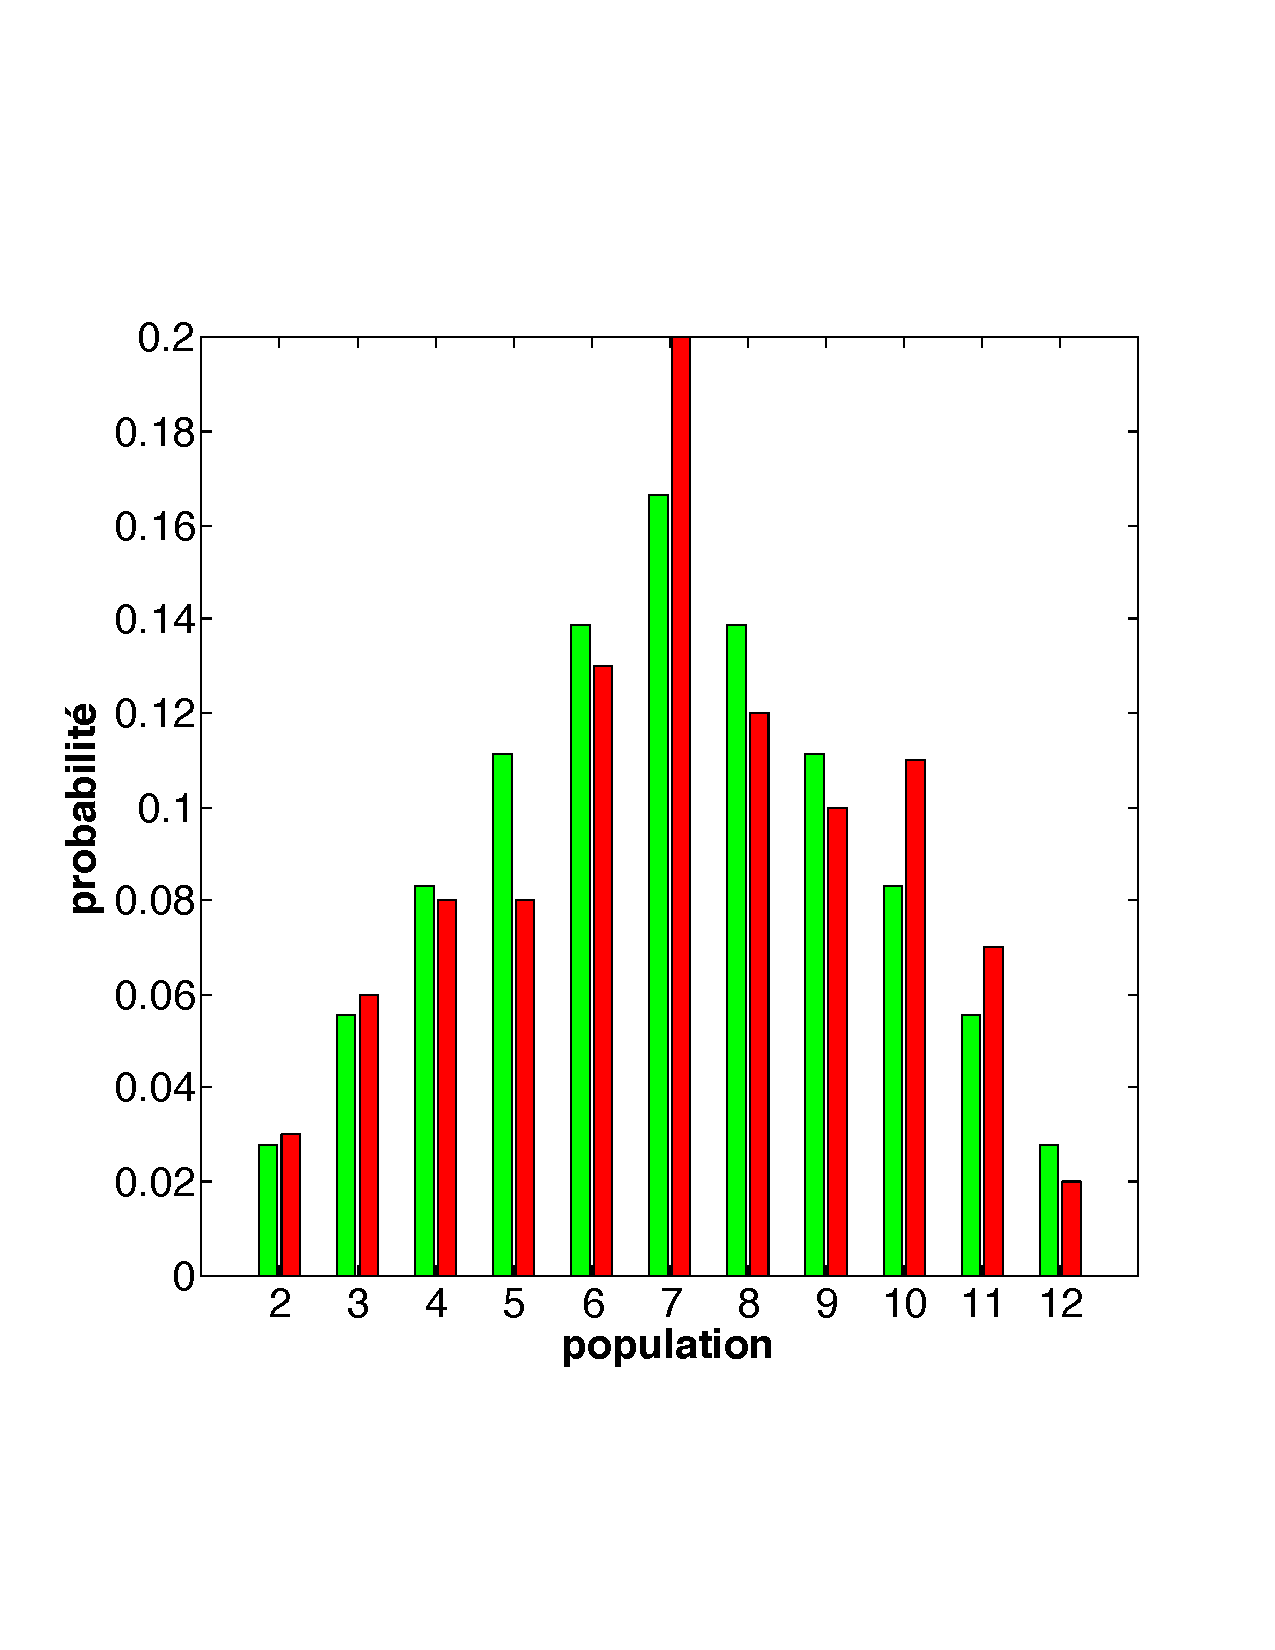
\includegraphics[width=6cm]{assets/figures/Serie2_exe01fig2.pdf}
	\caption{Distribution après 100 jets de dés (en rouge).}
	\label{fig:exe1fig2}
\end{wrapfigure}
\paragraph{Asymétrie et aplatissement.} Les formules du cours donnent
\begin{gather}
\beta_1=\frac{1}{\sigma_v^3}\sum\limits_{i=1}^{11}p(v_i)\,(v_i-\langle v \rangle)^3=0\\
\gamma_2=\frac{1}{\sigma_v^4}\sum\limits_{i=1}^{11}p(v_i)\,(v_i-\langle v \rangle)^4-3=-0.6343
\end{gather}

\paragraph{La probabilité} que $v\in[7\pm2.4152]$ est donnée par la somme de la probabilité de $v$ entre 4.5848 et 9.4152. Cependant, comme nous avons ici une distribution discrète, il n'y a pas beaucoup de sens à interpoler entre les valeurs de $p_i$, car les valeurs intermédiaires de $p_i$ ne représentent rien de réel. De fait, et en arrondissant $\sigma_v$ à l'unité la plus proche, soit 2, on peut calculer que la probabilité que $v\in[5,6,7,8,9]$ est égale à la somme $p(5)+p(6)+p(7)+p(8)+p(9)=(4+5+6+5+4)/36=24/36=2/3\approx 67\%$.

\paragraph{Vérification par l'expérience} On a jeté 100 fois deux dés, et relevé la somme des deux dés. Les occurrences des différents termes de la population ont été les suivants
\begin{flushright}
\begin{tabular}{r|ccccccccccc}
$v_i$ & 2 & 3 & 4 & 5 & 6 & 7 & 8 & 9 & 10 & 11 & 12 \\
test $p_i$ \%& 3 & 6 & 8 & 8 & 13 & 20 & 12 & 10 & 11 & 7 & 2 \\
théo. $p_i$\% & 3 & 6 & 8 & 11 & 14 & 17 & 14 & 11 & 8 & 6 & 3 \\
\end{tabular}
\end{flushright}
où l'on a arrondi la probabilité théorique à l'unité pour rendre la comparaison plus simple. On remarque que bien qu'il persiste encore quelque différences, les valeurs mesurées en pratique ont déjà bien convergé vers les valeurs théoriques attendues (fig. \ref{fig:exe1fig2}).

\subsection*{Solution de l'exercice 7.3}

\paragraph{Moyenne, écart-type :} on trouve
\begin{gather*}
\langle x \rangle=\sum_{i=1}^{10}p_i\,x_i=1.48\\
\langle x^2 \rangle=\sum_{i=1}^{10}p_i\,x_i^2=6.256\\
\sigma_x=\sqrt{\langle x^2 \rangle-\langle x\rangle^2}=\sqrt{4.0656}=2.0163\approx 2
\end{gather*}

\paragraph{Moments d'ordre 3 et 4 :} par définition, $\langle x^n\rangle=\sum_ip_i\,x_i^n$, d'où
\begin{gather*}
\langle x^3 \rangle=\sum_{i=1}^{10}p_i\,x_i^3=19.708\\
\langle x^4 \rangle=\sum_{i=1}^{10}p_i\,x_i^4=91.528
\end{gather*}

\paragraph{Le mode de X} est la valeur ayant la plus grande probabilité, soit $\text{mode}(X)=2$.

\paragraph{La fonction de répartition} $F(x)$ est la probabilité que la v.a. X soit inférieure ou égale à $x$. $F(x_i)$ est donnée par la somme des probabilités de toutes les valeurs inférieures ou égale à $x_i$. A partir du tableau de $p$, on trouve,
\begin{center}
\begin{tabular}{r|cccccccccc}
$i$ & 1 & 2 & 3 & 4 & 5 & 6 & 7 & 8 & 9 & 10 \\
$x_i$    &  -3 &   -2 &   -1 &    0 & 1    & 2    & 3    & 4    & 5   & 6\\
$p_i$ \% & 3.4 & 5.1 & 8.6 & 13.7 & 17.1 & 18.8 & 17.8 & 10.3 & 3.5 & 1.7 \\
$F_i$ \% & 3.4 & 8.5 & 17.1 & 30.8 & 47.9 & 66.7 & 84.5 & 94.8 & 98.3 & 100
\end{tabular}
\end{center}

\paragraph{La médiane} se trouve entre $x_5=1$ et $x_6=2$, valeurs pour lesquelles $F_5=47.9\%$ et $F_6=66.7\%$. Par interpolation, on trouve $(x_6-x_5)/(F_6-F_5)\times(50-F_5)+x_5=1/(66.7-47.9)\times(50-47.9)+1=1.1117$.

\paragraph{Le niveau de confiance} de l'intervalle $[\langle x\rangle\pm\sigma]=[1.48\pm2.0163]=[-0.5363,3.4963]$ est égale à la somme des probabilités que $x\in[\langle x\rangle\pm\sigma]$. Comme il s'agit d'une v.a. discrète, les probabilités des valeurs non discrètes n'ont pas de sens, ou sont nulles, donc
$$
P(x\in[-0.5363,3.4963])=p(0)+p(1)+p(2)+p(3)=13.7+17.1+18.8+17.8=67.4\ \%.
$$
Et pour le cas $x\in[\langle x\rangle\pm2\sigma]=[-2.5526,5.5126]$, on trouve
\begin{align*}
P(x\in[-2.5526,5.5126])&=p(-2)+p(-1)+p(0)+p(1)+p(2)+p(3)+p(4)+p(5)\\
&=5.1+8.6+13.7+17.1+18.8+17.8+10.3+3.5=94.9\ \%.
\end{align*}

\subsection*{Solution de l'exercice 7.3}

\paragraph{La probabilité totale} doit toujours être égale à 1 (ou 100 \%), sinon il ne s'agit pas d'une probabilité. Ici, nous sommes dans le cas d'une variable aléatoire \underline{continue}, dans le sens où toutes les valeurs réelles sont possibles, au contraire d'une v.a. discrète, où seules certaines valeurs sont possibles. Dans le cas d'une v.a. continue, les sommes deviennent des intégrales, et les bornes de l'intégrale sont celles du domaine de validité de la v.a. Dans le cas présent, la population de la v.a. est l'axe des réels, donc les intégrales sont à calculer de $-\infty$ à $+\infty$. Calculons la probabilité totale :
\begin{align*}
\int\limits_{-\infty}^{+\infty} p(U)\,\text{d}U=&
\int\limits_{-\infty}^{+\infty}\exp{(-2\,|U-U_0|)}\,\text{d}U=\cdots (z=U-U_0\Rightarrow\text{d}U=\text{d}z)\cdots
=\int\limits_{-\infty}^{+\infty}\exp{(-2\,|z|)}\,\text{d}z\\
=&2\int\limits_{0}^{+\infty}\exp{(-2\,z)}\,\text{d}z=2\left[-\frac{1}{2}\exp{(-2\,z)}\right]_{0}^{+\infty}=
-\Big[\exp{(-2\,z)}\Big]_{0}^{+\infty}=-(0-1)=1
\end{align*}
$p(U)$ est donc bien une distribution de probabilité.

\paragraph{Moyenne et écart-type} se calculent à partir de la définition du moment d'ordre $n$ de $U$,
$$
\langle U^n\rangle=\int\limits_{-\infty}^{+\infty} U^n\,p(U)\,\text{d}U
$$
et on trouve
\begin{align*}
\langle U \rangle=&\int\limits_{-\infty}^{+\infty} U\,\exp{(-2\,|U-U_0|)}\,\text{d}U=
\cdots z=U-U_0\Rightarrow\text{d}U=\text{d}z\cdots\\
=&\int\limits_{-\infty}^{+\infty} (z+U_0)\,\exp{(-2\,|z|)}\,\text{d}z
=\underbrace{\int\limits_{-\infty}^{+\infty} z\,\exp{(-2\,|z|)}\,\text{d}z}_{\text{fonction impaire, donc} \int=0}+
U_0\underbrace{\int\limits_{-\infty}^{+\infty} \exp{(-2\,|z|)}\,\text{d}z}_{\int p(U)\text{d}U=1}=U_0
\end{align*}
ce qui est normal, car la distribution de probabilité est symétrique autour de $U_0$. Quant à l'écart-type, on a
\begin{align*}
\langle U^2 \rangle=&\int\limits_{-\infty}^{+\infty} U^2\,\exp{(-2\,|U-U_0|)}\,\text{d}U=
\cdots z=U-U_0\Rightarrow\text{d}U=\text{d}z\cdots\\
=&\int\limits_{-\infty}^{+\infty} (z+U_0)^2\,\exp{(-2\,|z|)}\,\text{d}z
=\int\limits_{-\infty}^{+\infty} (z^2+2zU_0+U_0^2)\,\exp{(-2\,|z|)}\,\text{d}z\\
=&\int\limits_{-\infty}^{+\infty} z^2\,\exp{(-2\,|z|)}\,\text{d}z+
2U_0\underbrace{\int\limits_{-\infty}^{+\infty} z\,\exp{(-2\,|z|)}\,\text{d}z}_{=0}+
U_0^2\underbrace{\int\limits_{-\infty}^{+\infty} \exp{(-2\,|z|)}\,\text{d}z}_{=1}\\
=&\,2\int\limits_{0}^{+\infty} z^2\,\exp{(-2\,z)}\,\text{d}z+U_0^2=\cdots\text{double intégration par parties}\cdots=\frac{1}{2}+U_0^2
\end{align*}
par conséquent
$$
\sigma_U=\sqrt{\langle U^2 \rangle-\langle U\rangle^2}=\sqrt{1/2+U_0^2-U_0^2}=1/\sqrt{2}=0.707\approx 0.7
$$
\begin{wrapfigure}[13]{l}[0pt]{6cm}
   \centering
   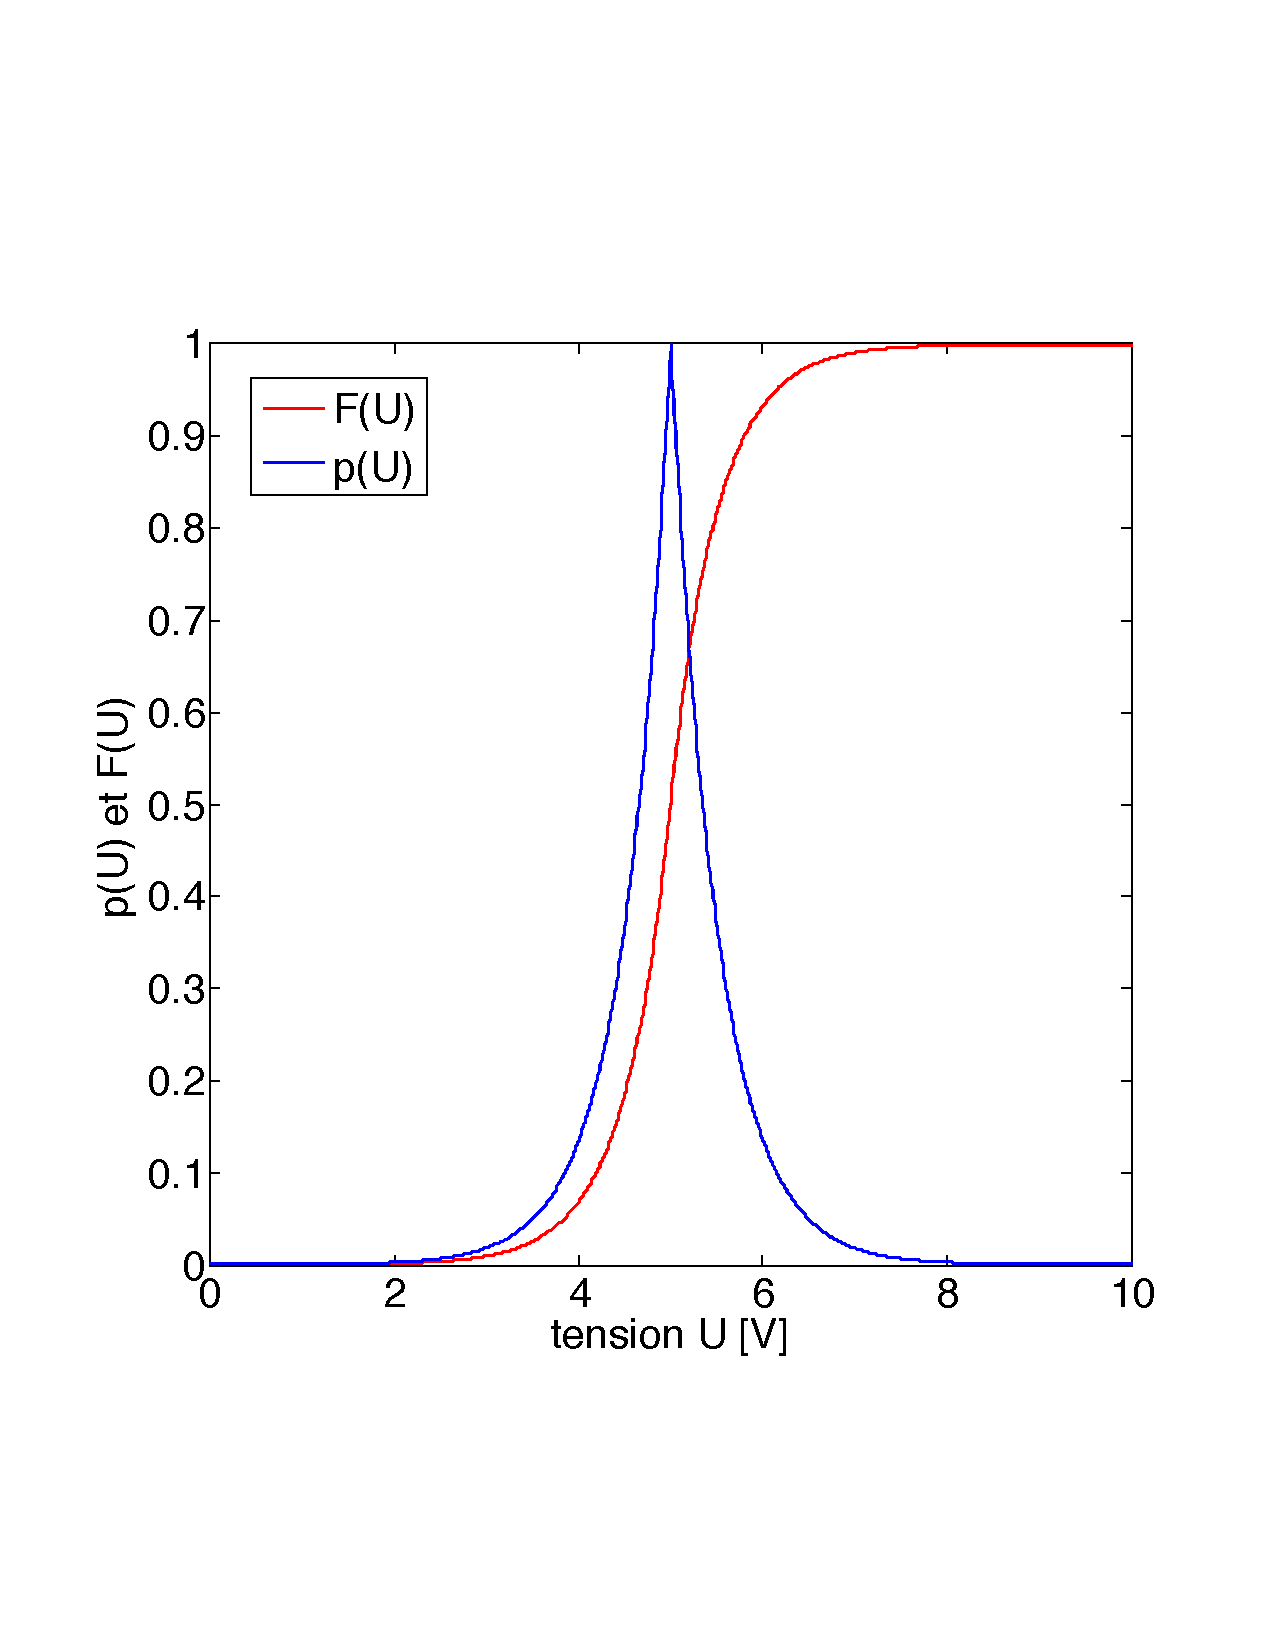
\includegraphics[height=6cm]{assets/figures/Serie2_exe09fig1.pdf}
   \caption{Distribution et fonction de répartition des tensions autour de la moyenne 5 V.}
   \label{fig:exe13}
\end{wrapfigure}

\paragraph{Le mode de la distribution} est la valeur la plus probable, soit, ici, $U_0$.

\paragraph{La fonction de répartition} en U est donnée par l'intégrale de $p(U)$ de $-\infty$ à $U$,
\begin{align*}
F(U)=\int\limits_{-\infty}^{U}\exp{(-2\,|U-U_0|)}\,\text{d}U
\end{align*}
et il vaut mieux séparer le calcul en deux parties : tout d'abord, si $U\le U_0$, alors, sachant que $|x|=-x$ lorsque $x\le 0$,
\begin{align*}
F(U\le U_0)&=\int\limits_{-\infty}^{U}\exp{[+2\,(U-U_0)]}\,\text{d}U\\
&=\frac{1}{2}
\exp{[2\,(U-U_0)]}\bigg|_{-\infty}^{U}=\frac{1}{2}\exp{[2\,(U-U_0)]},
\end{align*}
puis si $U>U_0$,
\begin{multline*}
F(U>U_0)=F(U_0)+\int\limits_{U_0}^{U}\exp{[-2\,(U-U_0)]}\,\text{d}U\\=\frac{1}{2}-\frac{1}{2}
\exp{[-2\,(U-U_0)]}\bigg|_{U_0}^{U}\\
=\frac{1}{2}-\frac{1}{2}\exp{[2\,(U-U_0)]}+\frac{1}{2}=1-\frac{1}{2}\exp{[2\,(U-U_0)]}
\end{multline*}

\paragraph{La médiane} est la valeur de la tension telle que la fonction de répartition est égale à 1/2, soit, ici $\text{med}(U)=U_0$. Pour ces mesures, moyenne, mode et médiane sont donc égales.

\paragraph{Le niveau de confiance} des intervalles de confiance à $U_0$ $\pm1\sigma_U$, $\pm2\sigma_U$ et $\pm3\sigma_U$ est donné, respectivement, par
\begin{align*}
p(|U-U_0|\le \sigma_U)&=\int\limits_{U_0-\sigma_U}^{U_0+\sigma_U}p(U)\,\text{d}U=
\int\limits_{U_0-\sigma_U}^{U_0+\sigma_U}\exp{(-2\,|U-U_0|)}\,\text{d}U=\cdots z=U-U_0\Rightarrow\text{d}U=\text{d}z\cdots\\
&=2\int\limits_{0}^{\sigma_U}\exp{(-2\,z)}\,\text{d}z=\cdots=1-\exp{(-2\,\sigma_U)}=
1-\exp{(-2/\sqrt{2})}=0.7569
\end{align*}
puis,
\begin{align*}
p(|U-U_0|\le 2\,\sigma_U)&=\cdots=1-\exp{(-4\,\sigma_U)}=0.9409\\
p(|U-U_0|\le 3\,\sigma_U)&=\cdots=1-\exp{(-6\,\sigma_U)}=0.9856
\end{align*}

\subsection*{Solution de l'exercice 7.4}

\begin{itemize}
\item Pour une distribution symétrique, mode, médiane et moyenne sont forcément identiques, ici égale à 73 photons.
\item La probabilité que le bruit soit positif, c-à-d la proportion de pixels où le bruit est positif, est égale à l'intégrale de la distribution pour les valeurs positives, soit, avec $\sigma_b=111$ photons et $\mu_b=73$ photons,
$$
P(b>0)=\int\limits_{0}^{\infty}p(b)\,\text{d}b=\frac{1}{73\sqrt{2\pi}}
\int\limits_{0}^{\infty}\exp{\left[-(b-73)^2/(2\cdot111^2)\right]}\,\text{d}b
$$
et avec un calcul numérique, on trouve $P(b>0)=0.675$. Quant à la probabilité d'obtenir un bruit négatif, il est donnée par $P(b<0)=1-P(b>0)=1-0.675=0.325$.
\item la largeur à mi-hauteur $\lambda_b$ est égale à deux fois la valeur de l'écart $\Delta b=b-73$ par rapport à la moyenne pour laquelle la distribution de Gauss est égale à 1/2 sa valeur maximale (en $\Delta b=0$); il faut donc résoudre l'équation
$$
p(\Delta b)=\frac{\text{max}(p(b))}{2}=\frac{1}{\sigma_b\,2\sqrt{2\pi}}
$$
il vient donc
$$
\frac{1}{\sigma_b\,\sqrt{2\pi}}\exp{\left[-(\Delta b)^2/(2\,\sigma_b^2)\right]}=\frac{1}{\sigma_b\,2\sqrt{2\pi}}
$$
c-à-d
$$
\exp{\left[-(\Delta b)^2/(2\,\sigma_b^2)\right]}=\frac{1}{2}
$$
d'où
$$
\Delta b=\sqrt{2\ln{2}}\,\sigma_b=1.177\,\sigma_b
$$
puis
$$
\lambda_b=2\sqrt{2\ln{2}}\,\sigma_b=2.355\,\sigma_b
$$
On trouve alors, numériquement, $\lambda_b=261.4$ photons.
\item pour une distribution gaussienne, le niveau de confiance associé à l'intervalle $[\mu_b\pm\sigma_b]$ est donné par l'intégrale de la distribution sur cet intervalle, et on trouve $\alpha_{1\,\sigma}=0.683$.
\item pour l'intervalle $[\mu_b\pm\lambda_b/2]$, cette même intégration conduit à $\alpha=0.761$.
\end{itemize}

\subsection*{Solution de l'exercice 7.5}

Trivial. On pose que la distribution = 1/2 et on résous l'équation.

\subsection*{Solution de l'exercice 7.6}

La distribution tends vers une gaussienne. Donc, dès qu'un système physique (une machine) comporte un grand nombre d'éléments indépendants et dont les caractéristiques sont susceptibles  de fluctuer, tout variable globale, fonction des variables internes, se comportera comme une variable aléatoire gaussienne. C'est pour cela que la distribution gaussienne est si fréquente.

\subsection*{Solution de l'exercice 7.7}

On trouve $2\Delta\mu=2\cdots0.005/100=10^{-4}$ mm.

\subsection*{Solution de l'exercice 7.8}

On a $\Delta\mu=0.001/3=3.\overline{3}\cdots10^{-4}$ mm, d'où $\sqrt{N}=0.005/3.\overline{3}\cdots10^{-4}=15$ et $N=225$.

%----------
\section{Solutions des exercices du chapitre 8}
%----------

%..........
\subsection*{Solution de l'exercice 8.1}
%..........

\subsubsection*{Cas à une variable, \textit{f = f(x)}}

Ici, on utilise la forme simple, au premier ordre, à savoir
$$
\Delta f=\left|\frac{\dd f}{\dd x}\right|\Delta x
$$

\begin{description}\renewcommand{\labelitemi}{$\bullet$}
\item[Energie du photon] $E=h\,c/\lambda$. Donnez $\Delta E$ en fonction de $\lambda$ et $\Delta\lambda$.\\
\textbf{Solution :} $\dd E/\dd\lambda=-h\,c/\lambda^2$, d'où $\Delta E=(h\,c/\lambda^2)\Delta\lambda$
\item[Décibels et puissance] $dB=20\log{P/P_0}$. Calculez $\Delta dB$ en fonction de $\Delta P$ et de $P$.\\
\textbf{Solution :} avec $\log_a x=\ln x / \ln a$ et $\dd(\ln x)/\dd x=1/x$ il vient $\dd(\log_a x)/\dd x=1/(x\ln a)$ et donc, avec $P_0$ constante,
$$
\frac{\dd(dB)}{\dd P}=20\,\frac{\dd}{\dd P}(\log{P}-\log{P_0})=\frac{20}{P\ln{10}}
$$
d'où
$$
\Delta(dB)=\frac{20}{\ln{10}}\frac{\Delta P}{P}=8.686\,\frac{\Delta P}{P}
$$
\end{description}

\subsubsection*{Cas à deux variables indépendantes, \textit{f = f(x,y)}}

Ici, puisque les deux variables sont indépendantes, on utilisera
$$
\Delta f=\sqrt{\left|\frac{\dd f}{\dd x}\right|^2(\Delta x)^2+\left|\frac{\dd f}{\dd y}\right|^2(\Delta y)^2}
$$
\begin{description}\renewcommand{\labelitemi}{$\bullet$}
\item[loi d'Ohm] $U=R\,I$, calculez $\Delta U$ en fonction de $R$, $\Delta R$, $I$ et $\Delta I$.\\
\textbf{Solution :} ici c'est assez simple,
$$
(\Delta U)^2=\left|\frac{\dd U}{\dd R}\right|^2(\Delta R)^2+\left|\frac{\dd U}{\dd I}\right|^2(\Delta I)^2 \Longrightarrow \Delta U=\sqrt{I^2(\Delta R)^2+R^2(\Delta I)^2}
$$
\item[Période d'oscillation masse et ressort] $T=2\pi\sqrt{m/k}$. Calculez $\Delta T$ en fonction de $m$, $\Delta m$, $k$, $\Delta k$.\\
\textbf{Solution :}
$$
\frac{\dd T}{\dd m}=\frac{\pi}{\sqrt{k\,m}}\ \ \text{et}\ \ \frac{\dd T}{\dd k}=-\frac{\pi\sqrt{m}}{k\sqrt{k}}
$$
d'où
\begin{gather*}
(\Delta T)^2=\frac{\pi^2}{k\,m}(\Delta m)^2+\frac{\pi^2\,m}{k^3}(\Delta k)^2=
\frac{\pi^2\,m}{k}
\left[\left(\frac{\Delta m}{m}\right)^2+\left(\frac{\Delta k}{k}\right)^2\right]\\
\Delta T=\frac{T}{2}
\sqrt{\left(\frac{\Delta m}{m}\right)^2+\left(\frac{\Delta k}{k}\right)^2}
\end{gather*}
\item[Loi de Snell (optique)] $n_2\sin{\theta_2}=n_1\sin{\theta_1}$. Calculez $\Delta\theta_2$ en fonction de $\theta_1$, $\Delta\theta_1$, $n_1$, $\Delta n_1$, $n_2$, $\Delta n_2$.\\
\textbf{Solution :}
avec
\begin{equation}
\theta_2=\sin^{-1}{\left(\frac{n_1}{n_2}\sin{\theta_1}\right)}\\
\end{equation}
il vient, en utilisant une formulation compacte,
\begin{gather*}
\frac{\dd\theta_2}{\dd\theta_1}=\frac{1}{\sqrt{1-\left(\frac{n_1}{n_2}\sin{\theta_1}\right)^2}}
\frac{n_1}{n_2}\cos{\theta_1}=\frac{n_1\cos{\theta_1}}{n_2\cos{\theta_2}}\\
\frac{\dd\theta_2}{\dd n_1}=\frac{1}{\sqrt{\dots}}\frac{\sin{\theta_1}}{n_2}=
\frac{\sin{\theta_1}}{n_2\cos{\theta_2}}=\frac{\sin{\theta_1}}{n_1\cos{\theta_1}}\cdot\frac{n_1\cos{\theta_1}}{n_2\cos{\theta_2}}=
\frac{\tan{\theta_1}}{n_1}\cdot\frac{n_1\cos{\theta_1}}{n_2\cos{\theta_2}}\\
\frac{\dd\theta_2}{\dd n_2}=\frac{1}{\sqrt{\dots}}n_1\sin{\theta_1}(-1)n_2^{-2}=
-\frac{n_1\sin{\theta_1}}{n_2^2\cos{\theta_2}}=
-\frac{\tan{\theta_1}}{n_2}\cdot\frac{n_1\cos{\theta_1}}{n_2\cos{\theta_2}}
\end{gather*}
par conséquent,
\begin{gather*}
(\Delta\theta_2)^2=\left(\frac{n_1\cos{\theta_1}}{n_2\cos{\theta_2}}\right)^2
\left[(\Delta\theta_1)^2+
\left(\frac{\tan{\theta_1}}{n_1}\right)^2(\Delta n_1)^2+
\left(\frac{\tan{\theta_1}}{n_2}\right)^2(\Delta n_2)^2\right]\\
\Delta\theta_2=
\frac{n_1\cos{\theta_1}}{n_2\cos{\theta_2}}
\sqrt{(\Delta\theta_1)^2+\tan^2{\theta_1}
\left[\left(\frac{\Delta n_1}{n_1}\right)^2+\left(\frac{\Delta n_2}{n_2}\right)^2\right]}
\end{gather*}
\end{description}

%..........
\subsection*{Solution de l'exercice 8.2}
%..........

On va rappeler et généraliser un résultat du cours. On sait que pour un quotient $f(x,y)=x/y$ on aura que
$$
\left(\frac{\Delta f}{f}\right)^2=\left(\frac{\Delta x}{x}\right)^2+
\left(\frac{\Delta y}{y}\right)^2
$$
or ceci est aussi valable pour un quotient $f(x,y)=a\,x/y$, en effet :
$$
\left(\frac{\Delta f}{f}\right)^2=
\left(\frac{\Delta(a\,x)}{a\,x}\right)^2+\left(\frac{\Delta y}{y}\right)^2=
\left(\frac{a\,\Delta x}{a\,x}\right)^2+\left(\frac{\Delta y}{y}\right)^2=
\left(\frac{\Delta x}{x}\right)^2+\left(\frac{\Delta y}{y}\right)^2
$$
Par ailleurs, puisque pour
$$f(x)=x^n$$
on a
$$\frac{\dd f}{f}=n\frac{\dd x}{x}$$
on trouve le résultat général suivant : pour une fonction
$$f(x,y)=a\,x^n\,y^m$$
l'incertitude relative s'écrit
$$
\left(\frac{\Delta f}{f}\right)^2=
n^2\,\left(\frac{\Delta x}{x}\right)^2+m^2\,\left(\frac{\Delta y}{y}\right)^2
$$
et la constante $a$ n'apparaît pas dans l'incertitude relative.

Revenons à notre problème (nous n'avons en fait pas besoin de la formule générale ci-dessus pour cet exercice, mais j'ai pris cette opportunité pour l'introduire). Il vient
$$
\left|\frac{\Delta N}{N}\right|=
\sqrt{\left(\frac{\Delta P}{P}\right)^2+\left(\frac{\Delta T}{T}\right)^2}
$$
numériquement
$$
\left|\frac{\Delta N}{N}\right|=
\sqrt{\left(\frac{10}{616}\right)^2+\left(\frac{3}{277}\right)^2}=0.019515
$$
on garde autant de chiffres significatifs que l'on veut pour le moment. Ensuite,
$$
\langle N \rangle=\alpha\frac{\langle P \rangle}{\langle T \rangle}
=80\cdot10^{-6}\text{[K$\cdot$m$^2$/N]}\,\frac{\text{616 [mb]$\cdot$100 [N$\cdot$m$^{-2}\cdot$mb$^{-1}$]}}{\text{277 [K]}}=0.0177906
$$
par conséquent
$$
\Delta N=0.019515\times0.0177906=0.0003
$$
et on ne garde ici qu'un seul chiffre significatif sur l'incertitude. Finalement, on aura
$$
N=0.0178\pm0.0003\text{  [1]}
$$
ou encore mieux,
$$
N=(178\pm3)\cdot 10^{-4}\text{  [1]}
$$

%..........
\subsection*{Solution de l'exercice 8.3}
%..........

Les quatre grandeurs d'influence ci-dessus sont totalement indépendantes, par conséquent leurs incertitudes s'additionnent de manière quadratique (ou en d'autres termes, la variance totale est simplement la somme des variances de chaque composante, sans termes croisées, de corrélation nulle), et il vient
$$
\Delta D=\sqrt{3^2+1.5^2+0.8^2+2^2}=3.986\approx 4\ \mu\text{m}
$$

%..........
\subsection*{Solution de l'exercice 8.4}
%..........

\subsubsection*{Corrélation totale}

Dans le cas d'une corrélation totale, l'incertitude sur la fonction de x et y est donnée par la somme des incertitudes provenant de chaque composante, soit
$$
\Delta f=\left|\frac{\partial f}{\partial x}\right|\Delta x+
\left|\frac{\partial f}{\partial y}\right|\Delta y
$$
et dans le cas où $f$ est proportionnel à $x^n$ et/ou $y^m$, on a
$$
\left|\frac{\Delta f}{f}\right|=\left|n\frac{\Delta x}{x}\right|+\left|m\frac{\Delta y}{y}\right|
$$
L'application aux fonctions ci-dessus nous donne
\begin{gather*}
\Delta f_1=|\cos{(x)}|\Delta x+|\sin{(y)}|\Delta y\\
\Delta f_2=\left|\frac{\Delta x}{x}\right|+\left|\frac{\Delta y}{y}\right|\\
\Delta f_3=\left|\frac{x(xy+2)}{(1+xy)^2}\right|\Delta x+
\left|\frac{x^3}{(1+xy)^2}\right|\Delta y\\
\Delta f_4=2\exp(x^2-y^2)(|x|\Delta x+|y|\Delta y)\\
\left|\frac{\Delta f_5}{f_5}\right|=3\left|\frac{\Delta x}{x}\right|+2\left|\frac{\Delta y}{y}\right|
\end{gather*}

\subsubsection*{Variables indépendantes}

Si $x$ et $y$ sont indépendants, l'incertitude sur $f(x,y)$ est donnée par la somme \underline{quadratique} des incertitudes, soit
$$
\Delta f=\sqrt{\left|\frac{\partial f}{\partial x}\right|^2(\Delta x)^2+
\left|\frac{\partial f}{\partial y}\right|^2(\Delta y)^2}
$$
et dans le cas où $f$ est proportionnel à $x^n$ et/ou $y^m$, on a
$$
\left|\frac{\Delta f}{f}\right|=\sqrt{\left|n\frac{\Delta x}{x}\right|^2+
\left|m\frac{\Delta y}{y}\right|^2}
$$
L'application aux fonctions ci-dessus donne
\begin{gather*}
\Delta f_1=\sqrt{\cos^2{(x)}(\Delta x)^2+\sin^2{(y)}(\Delta y)^2}\\
\Delta f_2=\sqrt{\frac{(\Delta x)^2}{x^2}+\frac{(\Delta y)^2}{y^2}}\\
\Delta f_3=\frac{x\sqrt{(xy+2)^2(\Delta x)^2+x^4(\Delta y)^2}}{(1+xy)^2}\\
\Delta f_4=2\exp(x^2-y^2)\sqrt{x^2(\Delta x)^2+y^2(\Delta y)^2}\\
\left|\frac{\Delta f_5}{f_5}\right|=\sqrt{9\frac{(\Delta x)^2}{x^2}+4\frac{(\Delta y)}{y^2}}
\end{gather*}

%----------
\section{Solutions des exercices du chapitre 9}
%----------

%..........
\subsection*{Solution de l'exercice 9.1}
%..........

\begin{wrapfigure}[12]{l}[0pt]{6cm}
   \centering
	\vspace{-5mm}
   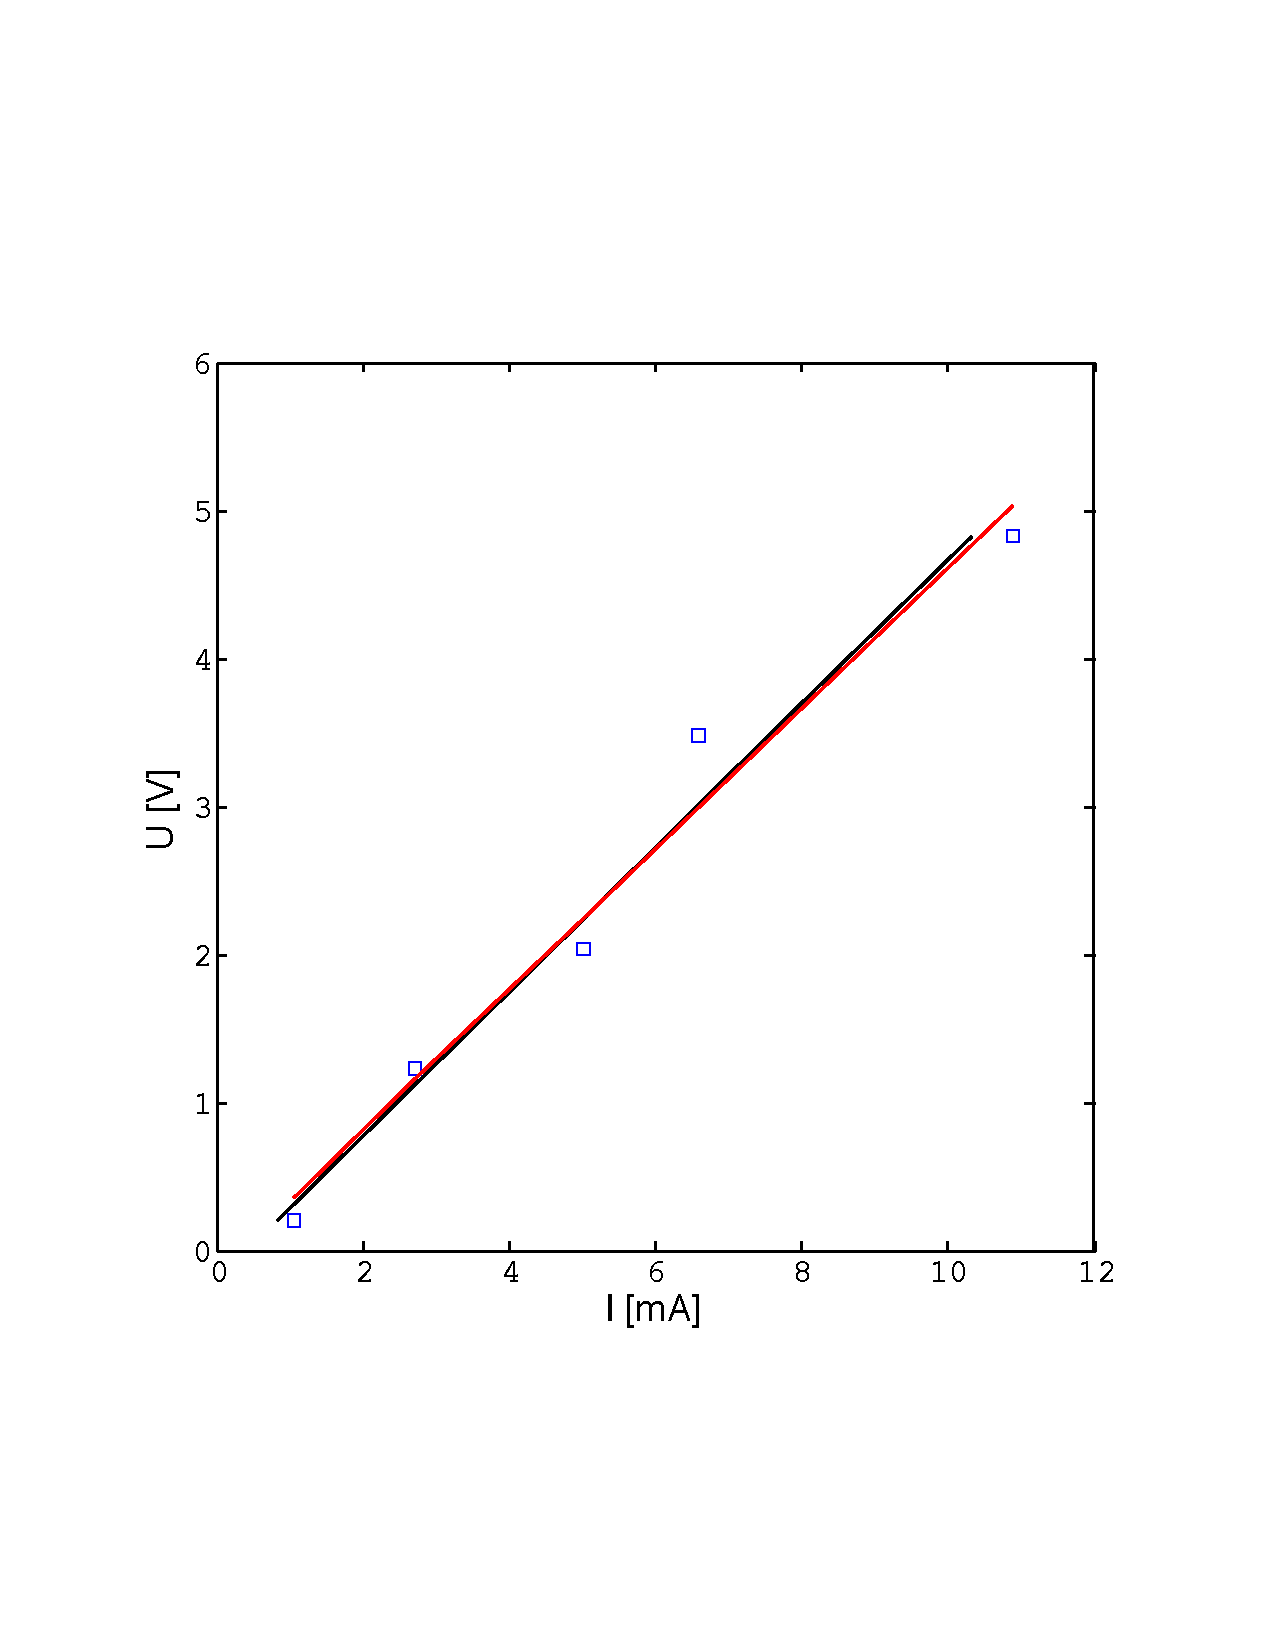
\includegraphics[width=6cm]{assets/figures/exe5.pdf}
   \caption{Mesures courant-tension et droite de régression directe (rouge) et inverse (noir).}
   \label{fig:03}
\end{wrapfigure}
Au cours, nous avons donné les formules pour le coefficient de corrélation linéaire ainsi que pour la pente $a$ et l'ordonnée à l'origine $b$ de la droite de régression $y=ax+b$, en fonction des statistiques sur les mesures des variables $x$ et $y$,
\begin{equation*}
a=r\,\frac{\sigma_y}{\sigma_x}\hspace{2cm}b=\langle y \rangle-a\,\langle x \rangle\\
\end{equation*}
avec
\begin{gather*}
r=\frac{\text{cov}(x,y)}{\sigma_x\sigma_y}\\
\sigma_x^2=\frac{1}{n}\sum_ix_i^2-\left(\frac{1}{n}\sum_ix_i\right)^2=
\langle x^2\rangle-\langle x \rangle^2\\
\sigma_y^2=\frac{1}{n}\sum_iy_i^2-\left(\frac{1}{n}\sum_iy_i\right)^2=
\langle y^2\rangle-\langle y \rangle^2\\
\text{cov}(x,y)=\frac{1}{n}\sum_ix_iy_i-\frac{1}{n}\sum_ix_i\frac{1}{n}\sum_iy_i=
\langle xy\rangle-\langle x \rangle\langle y \rangle
\end{gather*}
où la somme se fait sur le nombre de points de mesure, ici 5. Appliquons cela à notre problème. On trouve
\begin{center}
\begin{tabular}{ll}
$\langle I \rangle=5.256$ mA & $\langle U \rangle=2.3568$ V\\
$\langle I^2 \rangle=39.18788$ mA$^2$ & $\langle U^2\rangle=8.2310832$ V$^2$
\end{tabular}
\end{center}
donc
$$
\sigma_I=3.40034469\ \text{mA}\hspace{1cm}\sigma_U=1.6360247\ \text{V}
$$
puis
$$
\langle IU \rangle=17.87616\ \text{mA$\cdot$V}\Longrightarrow\text{cov}(I,U)=\text{cov}(U,I)=
5.4888192\ \text{mA$\cdot$V}
$$
on obtient alors
$$
r=0.987\hspace{1.5cm}a=0.47471509\ \text{V/mA}\hspace{1.5cm}b=-0.13830253\ \text{V}
$$
on donne ici un grand nombre de chiffres significatifs. Mais en fait, combien faudrait-il en garder ? Pour le trouver, il faudrait avoir une estimation de l'incertitude sur les mesures $I$ et $U$, et propager cette incertitude sur les calculs de $a$ et de $b$, à l'aide des équations ci-dessus, en suivant la même démarche que ce que nous avons fait dans les exercices 3 et 4, ce qui peut être assez fastidieux, mais parfois nécessaire. En l'absence de la connaissance des incertitudes sur les mesures, la règle est de donner 3 chiffres significatifs. On aura donc
$$
R=1000\,a=475\ \Omega\hspace{1.5cm}U_0=-0.138\ \text{V}
$$
On montre en figure \ref{fig:03} le résultat de l'ajustement de la droite de régression sur les points de mesure. On voit que la droite passe très proche de l'origine, et on peut se demander quelles serait la valeur de la pente si nous ajustions un modèle plus simple en $U=R\,I$, sans offset. Pour cela, il s'agit de trouver la valeur de la pente $a$ qui minimise l'écart quadratique suivant
$$
q^2=\sum\limits_{i=1}^{5}(U_i-a\,I_i)^2
$$
la solution est donnée par
$$
\frac{\dd q^2}{\dd a}=-2\sum\limits_{i=1}^{5}(U_i-a\,I_i)I_i=0
\Longrightarrow a=\frac{\sum\limits_{i=1}^{5}U_iI_i}{\sum\limits_{i=1}^{5}I_i^2}=
\frac{\langle UI\rangle}{\langle I^2\rangle}=\frac{17.87616}{39.18788}=0.45616552\ \text{V/mA}
$$
soit une valeur de la résistance $R=456\ \Omega$.

Pour déterminer la résistance $R$, nous avons choisi d'ajuster la droite $U=aI+b$, ce qui semble l'approche la plus intuitive. Cependant, nous aurions très bien pu, dans le cas présent, ajuster la droite inverse $I=aU+b$, et prendre l'inverse de $a$ pour déterminer $R$. Cette démarche, qui consiste à ajuster une droite de régression dans les deux sens, permet de déterminer une incertitude sur la pente la droite, et est souvent utilisée lorsque l'on a aucune information sur les incertitudes des mesures. Dans notre cas, on trouve, avec la droite inverse, et en utilisant les mêmes résultats sur la statistique de $U$ et de $I$, qui bien sûr sont les mêmes que dans le cas de la droite directe,
$$
a=r\frac{\sigma_I}{\sigma_U}=2.05068611\ \text{mA/V}\hspace{1cm}
b=\langle I \rangle-a\,\langle U \rangle=0.42294297\ \text{mA}
$$
La droite inverse est aussi représentée sur la figure \ref{fig:03}, et on voit qu'elle est tout de même très proche de la droite directe. La résistance déduite de la régression inverse est alors $R=1000/a=488\ \Omega$. On peut alors annoncer le résultat final, en prenant la moyenne des deux valeurs de la résistance, $R=481.5\pm6.5\ \Omega$, où on a considéré le demi-intervalle entre $R_{\text{max}}$ et $R_{\text{min}}$ comme une estimation (grossière) de l'incertitude. En appliquant la règle de 1 seul chiffre significatif pour l'incertitude, on écrira $R=482\pm7\ \Omega$.

%..........
\subsection*{Solution de l'exercice 9.2}
%..........

\begin{figure}[htb]
   \centering
   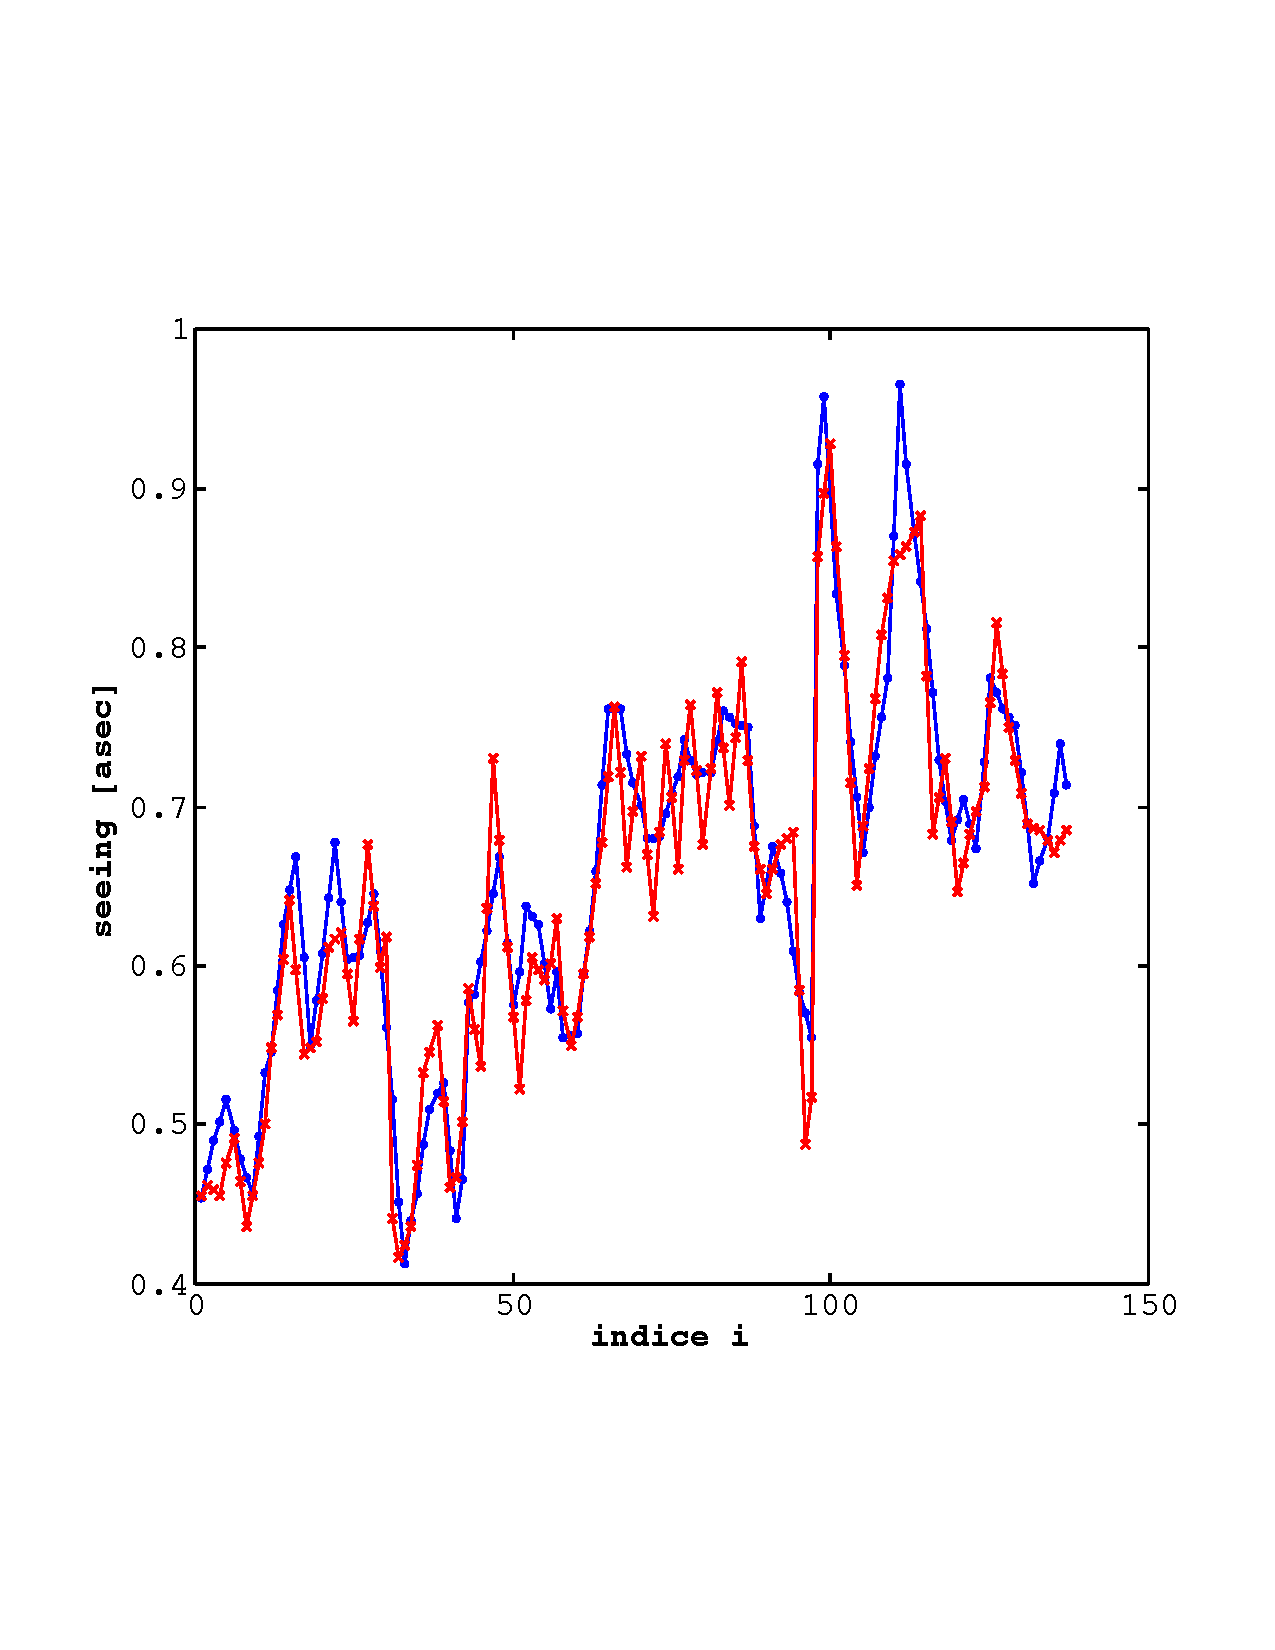
\includegraphics[height=7cm]{assets/figures/exe60.pdf}\hspace{10mm}
   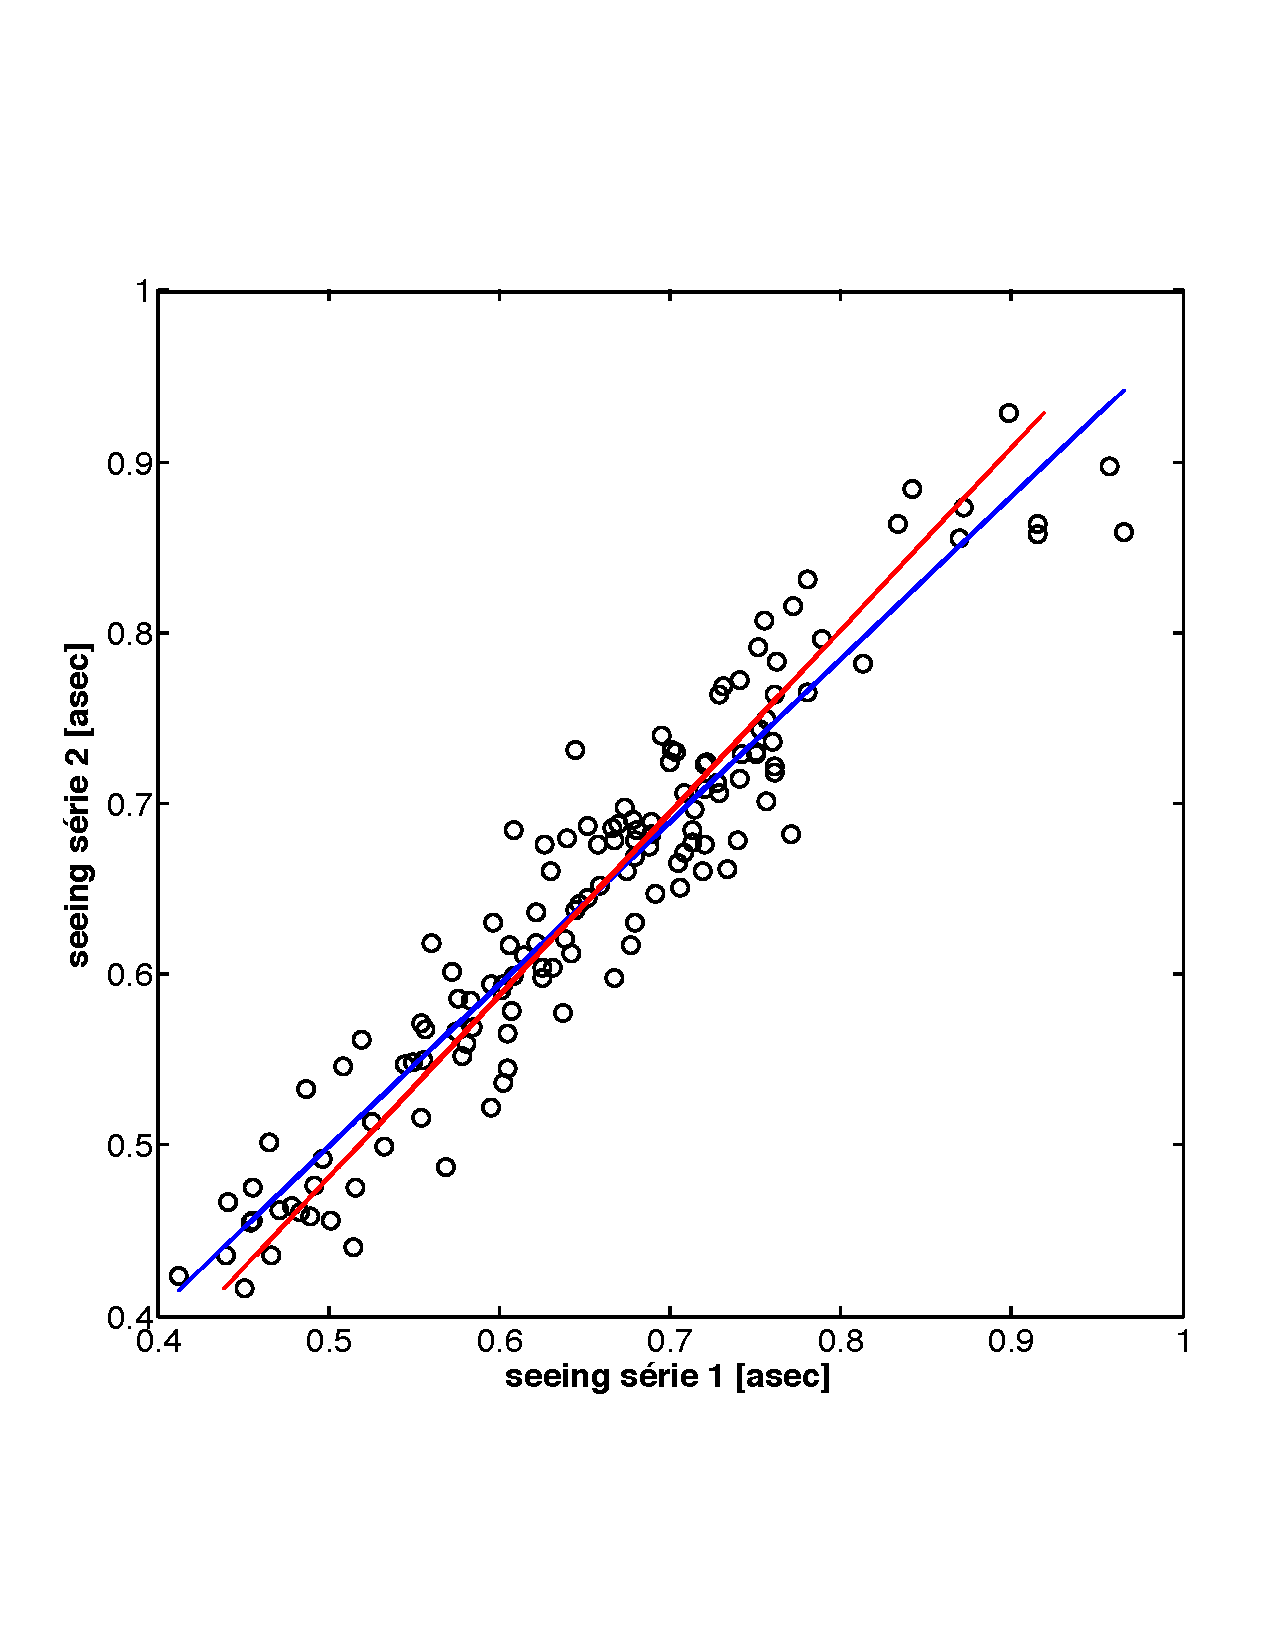
\includegraphics[height=7cm]{assets/figures/exe6.pdf}
   \caption{Gauche : évolution temporelle des deux séries de mesures, acquises en même temps. Droite : comparaison des deux séries, et droite de régression directe (rouge) et inverse (bleue).}
\end{figure}
En utilisant les formules rappelées lors de l'exercice 5, il vient
\begin{gather*}
\langle x \rangle=0.6540"
\hspace{0.5cm}\langle y \rangle=0.6454"
\hspace{0.5cm}\langle x^2 \rangle=0.4406^{"^{2}}\\
\hspace{0.5cm}\langle y^2 \rangle=0.4296^{"^{2}}
\hspace{0.5cm}\langle xy \rangle=0.4345^{"^{2}}
\hspace{0.5cm}\text{cov}(x,y)=0.01238^{"^{2}}
\end{gather*}
d'où
$$
\sigma_x=0.1135"\hspace{0.5cm}\sigma_y=0.1145"\hspace{0.5cm}r=0.9441
$$

\subsubsection*{Remarque : statistique à partir d'un échantillon de taille finie}

La théorie donnée plus haut pour le calcul du coefficient de corrélation et des paramètres de la droite de régression est basée sur l'hypothèse que l'on a un échantillon de dimension infinie (c'est-à-dire que l'on a réalisé une infinité de fois la même mesure), et que l'on dispose de ce fait d'une connaissance exacte de la statistique du mesurande (moyenne, écart-type etc). Or, les échantillons réels sont toujours de dimension finie, par conséquent on commet toujours une petite erreur lors de l'estimation des propriétés statistiques à partir d'un nombre fini de mesures. En d'autres termes, $N_{ech}$ n'a, en général, pas encore convergé vers l'infini.

Pour le calcul de la moyenne, on peut montrer qu'il n'y a pas vraiment de problème, et que la moyenne de l'échantillon de taille finie est une bonne estimation de la vraie moyenne (celle que nous obtiendrions si $N_{ech}\rightarrow\infty$). En revanche, pour la variance, on montre que l'écart quadratique moyen n'est pas un bon estimateur, si la variable aléatoire est gaussienne : cependant, cet effet peut être corrigé, et que la meilleure estimation de la variance d'une v.a. gaussienne, à partir d'un échantillon de taille finie, est donné par
$$
\text{estimateur}(\sigma_x^2)=\left(\frac{N_{ech}}{N_{ech}-1}\right)\times\text{écart quadratique moyen}
$$
et bien entendu, dans la limite $N_{ech}\rightarrow\infty$, l'écart quadratique moyen converge exactement vers la variance.

Le programme \texttt{Matlab} calcule les variances en utilisant la correction, et de ce fait, donne une valeur du coefficient de corrélation différente de ce que nous obtenons plus haut, $r_{\texttt{matlab}}=0.9524$. Nous utiliserons cependant uniquement nos formules, car l'utilisation des calculs via \texttt{Matlab} nécessiterait aussi la correction de la covariance, pour un gain de précision relativement modeste sur les coefficients de la droite de régression.

On trouve, pour la droite de régression directe, puis la droite de régression indirecte
$$
y=0.9524\,x+0.02249\hspace{1cm}x=0.9358\,y+0.5005
$$
l'inverse de la pente de la droite inverse est $1.0685$, ce qui nous donne en moyenne, entre les deux régressions, une pente de $1.01\pm0.03$ où on a considéré le demi-intervalle entre les deux valeurs comme un indicateur grossier d'incertitude.

Quoi qu'il en soit, on remarquera que cette pente moyenne est tout à fait compatible avec l'hypothèse que les deux séries de mesures de la résolution angulaire représentent une seule et même quantité. Les deux méthodes de mesure de la résolution angulaire peuvent donc être considérées comme deux méthodes équivalentes.

\subsubsection*{La médiane}

Pour calculer la médiane, c'est assez simple : il suffit d'ordonner les valeurs par ordre croissant, et de déterminer la valeur au centre de cette liste ordonnée. En effet, la médiane est la limite qui sépare en deux parties égales le nombre de valeurs inférieures et supérieures à elle-même. En exécutant la suite de commandes suivante,
\begin{flushleft}
\tt
[B,IX]=sort(x);\\
med=B((137-1)/2+1);\\
\end{flushleft}
\rm
où 137 est le nombre d'échantillons, on trouve une médiane de 0.6589" pour $x$ et de 0.6602" pour $y$. A remarquer que \texttt{Matlab} procède exactement de la même manière, car c'est exactement le résultat donné par la commande \texttt{median(x)}.

\subsubsection*{Le mode}

Avec le mode, les choses se compliquent. En effet, la valeur la plus fréquente va dépendre de  la largeur de la classe considérée, tout simplement parce qu'avec ces données, réelles, la forme de l'histogramme dépend de la classe, comme on le voit sur la figure \ref{fig:exe62}. Dans les deux cas représentés, le mode est de 0.76" pour la classe 0.024" et 0.68" pour la classe 0.0173", ce qui est tout de même fort différent. Dans ce cas, on conclura que le mode est un paramètre indéterminé pour cette série, en raison de la taille limitée de l'échantillon.
\begin{figure}[htb]
   \centering
   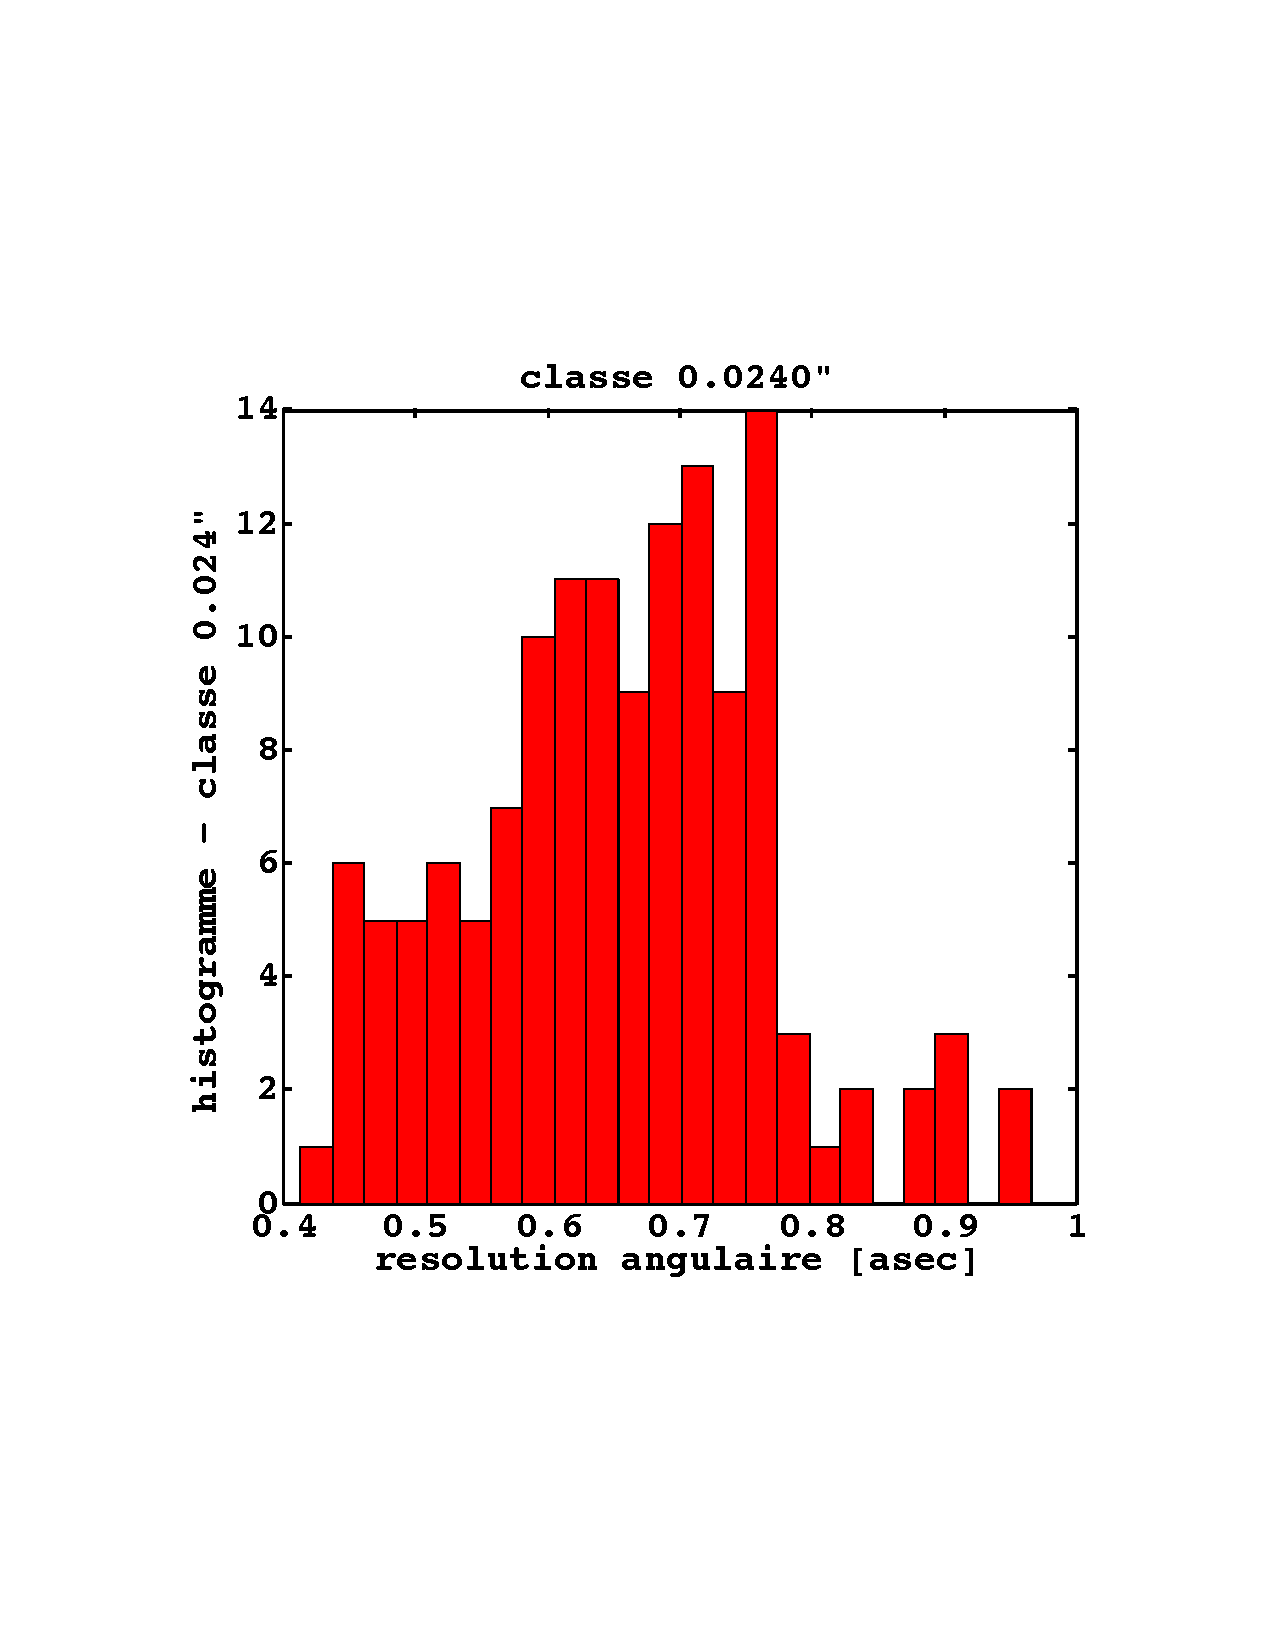
\includegraphics[height=7cm]{assets/figures/exe6hist1.pdf}\hspace{7mm}
   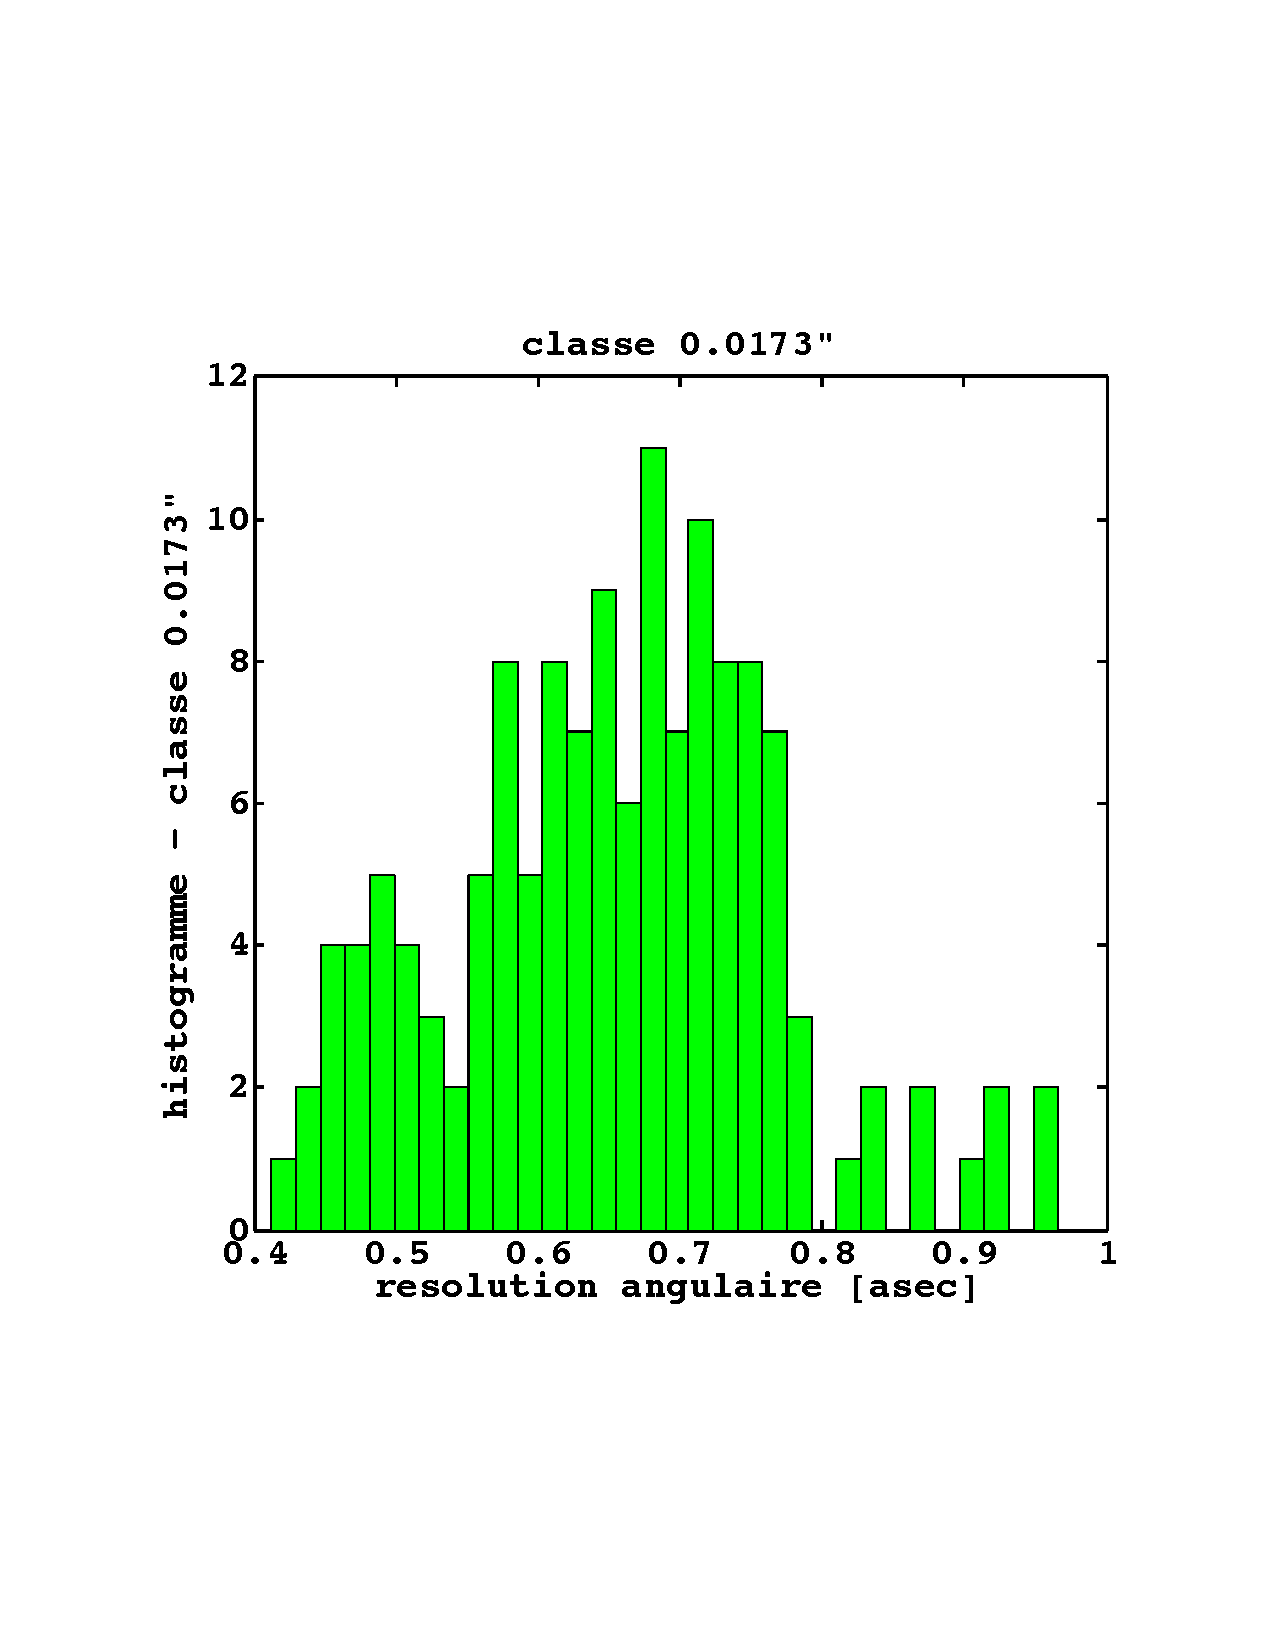
\includegraphics[height=7cm]{assets/figures/exe6hist2.pdf}
   \caption{Histogrammes de la série $x$ pour une classe de 0.024" (gauche) et de 0.0173" (droite). Les largeurs de classes sont proches, mais l'allure des histogrammes est assez différent.}
   \label{fig:exe62}
\end{figure}

%..........
\subsection*{Solution de l'exercice 9.3}
%..........

La régression polynomiale est un cas particulier d'ajustement de fonctions non linéaires. Une fonction linéaire est une fonction telle que $f(a_1x_1+a_2x_2+\cdots)=a_1f(x_1)+a_2f(x_2)+\cdots$, par exemple la relation $f(x)=ax+b$ est linéaire, tandis qu'une fonction non linéaire n'a pas cette propriété, comme par exemple la fonction $f(x)=\tan{x}$.

\subsubsection*{Rappel théorique}

Soit donc une série de $N_m$ points de mesures $(x_i,y_i)_{i=1\cdots N_m}$. On cherche à ajuster sur ces points une fonction d'équation connue, $y=f(x,\vec{p})$, mais dont on ignore les paramètres $\vec{p}$. L'ajustement va consister à trouver les paramètres $\vec{p}$ tels que $f(x,\vec{p})$ s'ajuste le mieux aux points mesurés $(x_i,y_i)_{i=1\cdots N_m}$.

L'idée est donc de minimiser l'écart quadratique total (ou moyen, c'est égal) entre les données et le modèle, minimisation que l'on trouve en posant que la dérivée de cet écart par rapport à chacun des paramètres $p_j$ est nulle,
$$
\frac{\partial}{\partial p_j}\sum\limits_{i=1}^{N_m}\big[f(x_i,\vec{p})-y_i\big]^2=0
$$
en développant, on trouve un système de $N_p$ équations, avec $N_p$ le nombre de paramètres
$$
\sum\limits_{i=1}^{N_m}\frac{\partial f(x_i,\vec{p})}{\partial p_j}f(x_i,\vec{p})=
\sum\limits_{i=1}^{N_m}\frac{\partial f(x_i,\vec{p})}{\partial p_j}y_i
$$
Puisque l'on a $N_p$ équations en $\vec{p}$, on peut en extraire à priori les $N_p$ paramètres inconnus. Mais pour cela, il faut que la fonction $f(x,\vec{p})$ soit linéaire par rapport à ses paramètres, de façon à ce que l'on puisse écrire un système de $N_p$ équations linéaires en $\vec{p}$. En effet, avec
$$
f(x,\vec{p})=p_1h_1(x)+p_2h_2(x)+\cdots+p_{N_p}h_{N_p}(x)
$$
où les fonctions individuelles $h_j(x)$ peuvent être quelconques, il est facile de voir que le système des $N_p$ équations devient
\begin{eqnarray*}
\frac{\partial }{\partial p_1} \text{:} &
\sum\limits_{j=1}^{N_p}\sum\limits_{i=1}^{N_m}p_j\,h_1(x_i)\,h_j(x_i)=
\sum\limits_{i=1}^{N_m}h_1(x_i)\,y_i\\
\frac{\partial }{\partial p_2} \text{:} &
\sum\limits_{j=1}^{N_p}\sum\limits_{i=1}^{N_m}p_j\,h_2(x_i)\,h_j(x_i)=
\sum\limits_{i=1}^{N_m}h_2(x_i)\,y_i\\
& \vdots\\
\frac{\partial }{\partial p_{N_p}} \text{:} &
\sum\limits_{j=1}^{N_p}\sum\limits_{i=1}^{N_m}p_j\,h_{N_p}(x_i)\,h_j(x_i)=
\sum\limits_{i=1}^{N_m}h_{N_p}(x_i)\,y_i\\
\end{eqnarray*}
et si on détaille la première ligne (par exemple)
$$
p_1\sum\limits_{i=1}^{N_m}h_1^2(x_i)+
p_2\sum\limits_{i=1}^{N_m}h_2(x_i)\,h_1(x_i)+
%p_3\sum\limits_{i=1}^{N_m}h_3(x_i)\,h_1(x_i)+
\cdots
p_{N_p}\sum\limits_{i=1}^{N_m}h_{N_P}(x_i)\,h_1(x_i)=
\sum\limits_{i=1}^{N_m}h_1(x_i)\,y_i
$$
on comprend alors que l'on peut écrire ce système sous la forme d'un produit de matrices,
\begin{equation*}
\begin{bmatrix}
\sum_i h_1^2(x_i)       & \sum_i h_2(x_i)h_1(x_i) & \cdots & \sum_i h_{N_p}(x_i)h_1(x_i)\\
\sum_i h_1(x_i)h_2(x_i) & \sum_i h_2^2(x_i)       & \cdots & \sum_i h_{N_p}(x_i)h_2(x_i)\\
\vdots & \vdots & \vdots & \vdots \\
\sum_i h_1(x_i)h_{N_p}(x_i) & \sum_i h_2(x_i)h_{N_p}(x_i) & \cdots & \sum_i h_{N_p}^2(x_i)
\end{bmatrix}
\begin{bmatrix} p_1 \\ p_2 \\ \vdots \\ p_{N_p}\end{bmatrix}=
\begin{bmatrix}
\sum_ih_1(x_i)\,y_i\\
\sum_ih_2(x_i)\,y_i\\
\vdots\\
\sum_ih_{N_p}(x_i)\,y_i
\end{bmatrix}
\end{equation*}
ou
$$
A\cdot\vec{p}=B
$$
La matrice $A$ et le vecteur $B$ se calculent numériquement à partir de la connaissance des fonctions $h_j(x)$ et des points de mesure $(x_i,y_i)$. La solution est donnée par
$$
\vec{p}=A^{-1}\cdot B
$$
Cependant, lorsque la fonction $f$ est non-linéaire par rapport à ses paramètres $\vec{p}$, il n'est généralement pas possible d'écrire le système matriciel ci-dessus et on doit se résoudre à utiliser une approche numérique, c'est-à-dire que l'on cherche par essai les valeurs $p_j$ qui minimisent l'écart quadratique.

Revenons à notre problème, et appliquons la théorie ci-dessus à la fonction-modèle pour nos données, la fonction $f(x)=\exp{(ax^2+bx+c)}$. Les paramètres du problème sont les coefficients $a,b,c$, soit ici $\vec{p}=[a,b,c]$. Tout d'abord, on remarquera que la fonction-modèle n'est \textit{pas} linéaire par rapport aux paramètres; par contre, la fonction $g(x)=\ln{f(x)}=ax^2+bx+c$, elle, l'est. On ajustera donc le modèle $g(x)$, mais non pas aux points $(x_i,y_i)$, mais aux points $(x_i,\ln{y_i})$.

%..........
\subsection*{Solution de l'exercice 9.4}
%..........

\paragraph{La transformation à appliquer} pour linéariser la relation est très simplement le logarithme, que l'on peut prendre dans n'importe quelle base, par exemple en base 10,
$$
z(\Delta t)=\log{n(\Delta t)}=\log{n_0}-\gamma\Delta t\log{2}
$$
en posant $a=-\gamma\log{2}$ et $b=\log{n_0}$, on trouve bien une relation linéaire en $\Delta t$, du type $y=ax+b$,
$$
z(\Delta t)=a\,\Delta t+b
$$
et en appliquant le log aux données $n(\Delta t)$, on a le nouveau tableau des données linéarisées,
\begin{center}
\begin{tabular}{r|cccccccccc}
$\Delta t$ [min] & 10 & 20 & 30 & 40 & 50 \\
$z(\Delta t)$ & 0.2772 & -0.0132 & -0.2916 & -0.6676 & -0.8633 \\\hline\hline
$\Delta t$ [min] & 60 & 70 & 80 & 90 & 100\\
$z(\Delta t)$ & -1.1871 & -1.4559 & -1.7696 & -2.2218 & -2.3979
\end{tabular}
\end{center}
Calculons le coefficient de corrélation linéaire
$$
r=\frac{\text{cov}(\Delta t,z)}{\sigma_{\Delta t}\,\sigma_z}
$$
avec
\begin{eqnarray*}
\text{cov}(\Delta t,z)&=&
\langle\Delta t\cdot z\rangle-\langle\Delta t\rangle\cdot\langle z\rangle\\
\sigma_{\Delta t}&=&\sqrt{\langle\Delta t^2\rangle-\langle\Delta t\rangle^2}\\
\sigma_{z}&=&\sqrt{\langle z^2\rangle-\langle z\rangle^2}\\
\end{eqnarray*}
on calcule
\begin{center}
\begin{tabular}{ccccc|ccccc}
$\langle\Delta t\rangle$ &
$\langle z\rangle$ &
$\langle\Delta t^2\rangle$ &
$\langle z^2\rangle$ &
$\langle\Delta t\cdot z\rangle$ &
$\text{cov}(\Delta t,z)$ &
$\sigma_{\Delta t}^2$ &
$\sigma_{z}^2$ &
$\sigma_{\Delta t}$ &
$\sigma_{z}$
\\\hline
55 & -1.0591 & 3850 & 1.8700 & -83.0572 & -24.8075 & 825 & 0.7483 & 28.7228 & 0.8651
\end{tabular}
\end{center}
ce qui nous donne $r=-0.9984$. La corrélation est donc excellente, ce qui nous permet de confirmer la validité du modèle de la décroissance du nombre de bactéries selon une loi en puissance de 2.

\paragraph{Les coefficients de la droite de régression} sont les suivants
\begin{gather*}
a=r\frac{\sigma_z}{\sigma_{\Delta t}}=-0.9984\,\frac{0.8651}{28.7228}=-0.03007\\
b=\langle z\rangle-a\langle\Delta t\rangle=0.5947
\end{gather*}
dont on déduit les paramètres du modèle (voir fig. \ref{fig:exe3fig1serie2}),
\begin{gather*}
\gamma=-a/\log{2}=0.099889\,(\approx0.1)\\
n_0=10^b=3.9332\,(\approx 4)
\end{gather*}
$n_0$ est le nombre moyen initial de bactéries avant traitement. Si on calcule les coefficients de la droite de régression inverse ($\Delta t = a' z +b'$) on trouve $a'=-33.1508$ soit $1/a'=-0.03017$, ce qui donne $\gamma=0.100207$. Le facteur $\gamma$ moyen, et son incertitude \textbf{estimée}, est donc
$$
\gamma=0.1000\pm0.0002
$$
ce facteur nous indique qu'après chaque tranche de 10 minutes de traitement, le nombre de bactéries actives est divisé par deux.

\paragraph{La durée de traitement} nécessaire (que l'on va noter $\tau$) pour qu'il ne reste en moyenne qu'une seule bactérie pour 100 mm$^2$ se calcule simplement avec notre modèle : 1 bactérie par 100 mm$^2$, c'est 0.01 bactérie par mm$^2$. Il faut donc que $4\cdot2^{-0.1\tau}=0.01$, soit $\tau=-\text{log}_2(0.01/4)/0.1=86.4$ minutes.

\begin{figure}[t]
   \centering
   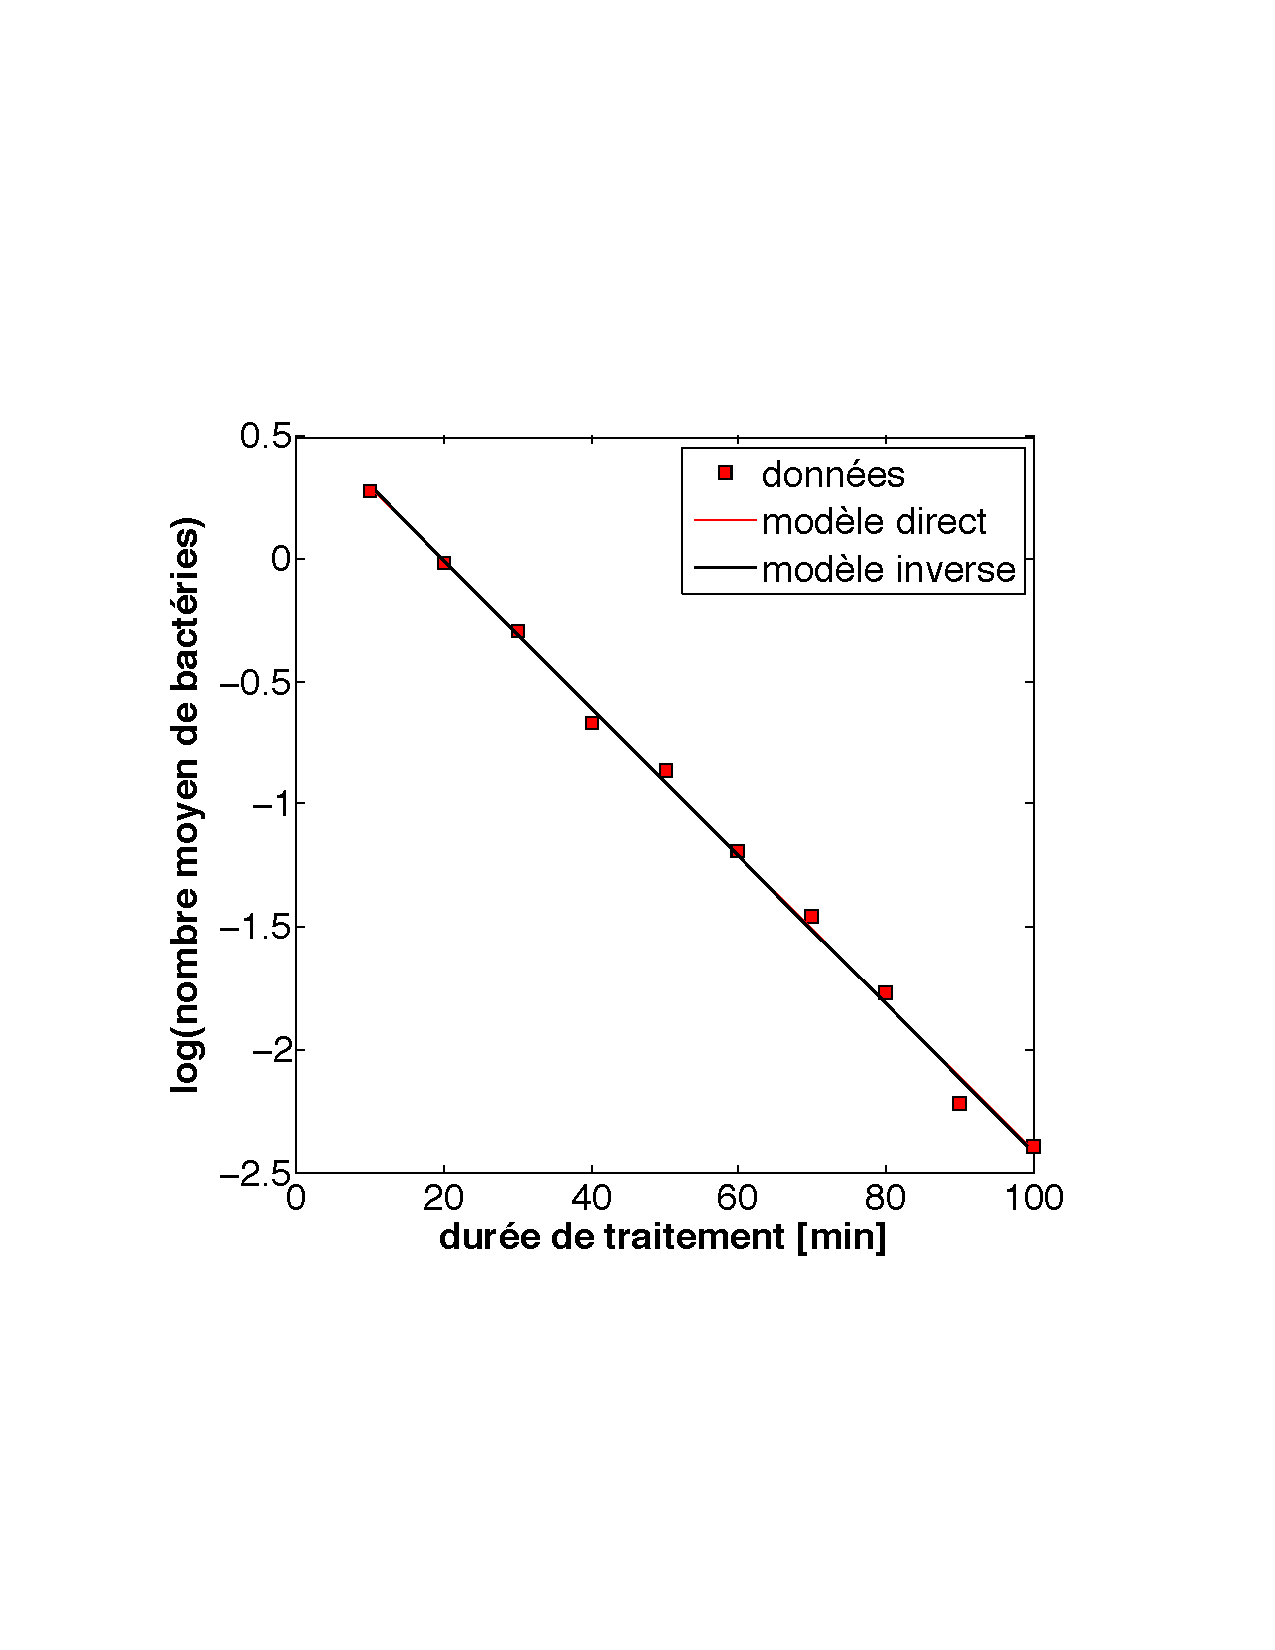
\includegraphics[height=7cm]{assets/figures/exe3fig1serie2.pdf}\hspace{7mm}
   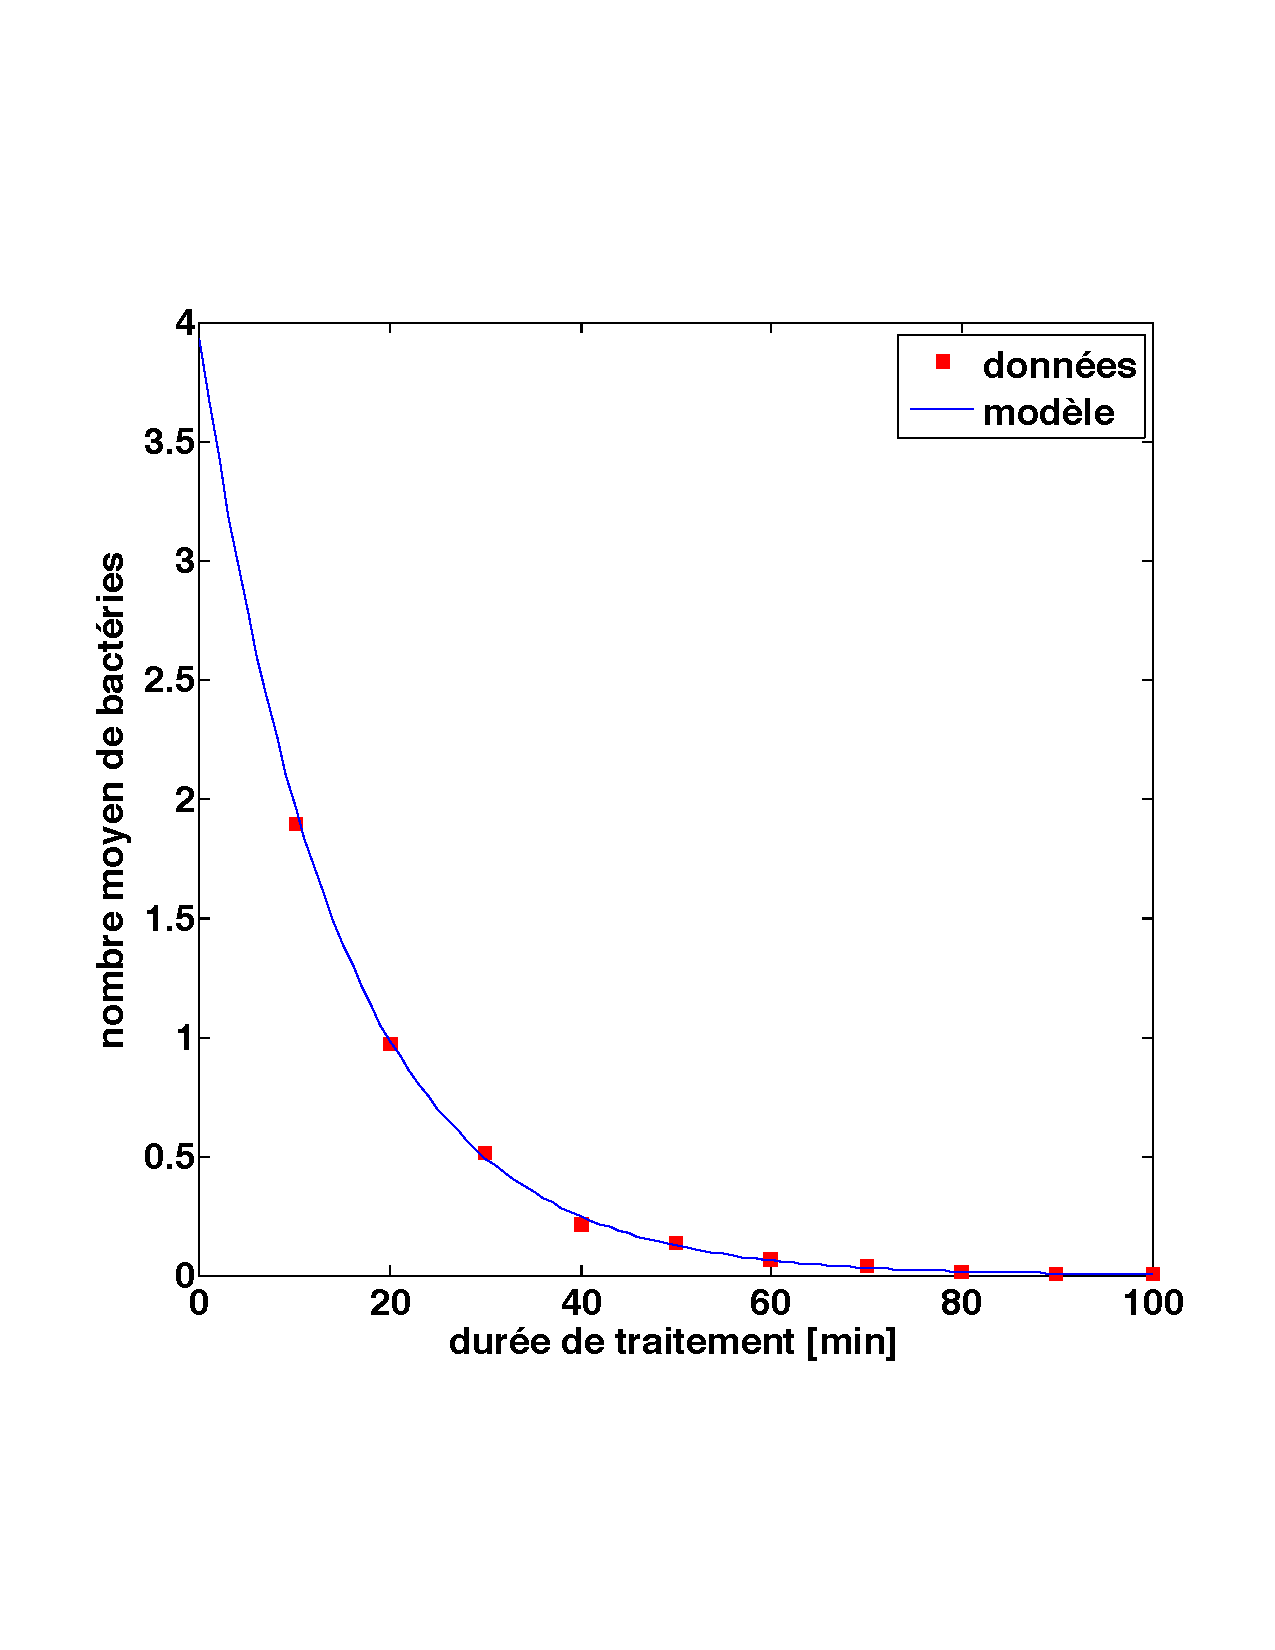
\includegraphics[height=7cm]{assets/figures/exe3fig2serie2.pdf}
   \caption{A gauche : données et modèle après linéarisation; A droite : données brutes et modèle final en puissance de 2. L'extrapolation à $\Delta t=0$ indique le nombre moyen de bactéries avant traitement.}
   \label{fig:exe3fig1serie2}
\end{figure}

%..........
\subsection*{Solution de l'exercice 9.5}
%..........

L'idée est donc de tester s'il existe une corrélation entre le nombre de naissances et la phase de la Lune. On va calculer le coefficient de corrélation linéaire entre $p$ et $n$. On applique la théorie (rappelée dans l'exercice 2), et on trouve
\begin{center}
\begin{tabular}{ccccc|cccc}
$\langle p\rangle$ & $\langle p^2\rangle$ & $\langle n\rangle$ & $\langle n^2\rangle$ &
$\langle p\cdot n\rangle$ & $\text{cov}(p,n)$ & $\sigma_p$ & $\sigma_n$ & r\\\hline
50 & 3541.7 & 12.1 & 163.9 & 629.2 & 23.61 & 32.275 & 4.149 & 0.176
\end{tabular}
\end{center}
La corrélation est donc très éloignée de l'unité, ce qui indique qu'il n'est pas possible d'affirmer qu'il existe une corrélation.

%..........
\subsection*{Solution de l'exercice 9.6}
%..........

La théorie est rappelée dans l'exercice 7 de la première série d'exercices. Les paramètres $[a,b,c,d]$ (un vecteur) sont donnés par la résolution du système
\begin{equation*}
\begin{bmatrix}
\sum_i h_1^2(x_i)       & \sum_i h_2(x_i)h_1(x_i) &
\sum_i h_3(x_i)h_1(x_i) & \sum_i h_4(x_i)h_1(x_i)\\
\sum_i h_1(x_i)h_2(x_i) & \sum_i h_2^2(x_i) &
\sum_i h_3(x_i)h_2(x_i) & \sum_i h_4(x_i)h_2(x_i)\\
\sum_i h_1(x_i)h_3(x_i) & \sum_i h_2(x_i)h_3(x_i) &
\sum_i h_3^2(x_i) & \sum_i h_4(x_i)h_3(x_i)\\
\sum_i h_1(x_i)h_4(x_i) & \sum_i h_2(x_i)h_4(x_i) & \sum_i h_3(x_i)h_4(x_i) & \sum_i h_4^2(x_i)
\end{bmatrix}
\begin{bmatrix} a \\ b \\ c \\ d\end{bmatrix}=
\begin{bmatrix}
\sum_ih_1(x_i)\,y_i\\
\sum_ih_2(x_i)\,y_i\\
\sum_ih_3(x_i)\,y_i\\
\sum_ih_4(x_i)\,y_i
\end{bmatrix}
\end{equation*}
avec
\begin{eqnarray*}
h_1(x)&=&x^3\\
h_2(x)&=&x^2\\
h_3(x)&=&x^1\\
h_4(x)&=&1
\end{eqnarray*}
il vient
\begin{equation*}
\begin{bmatrix}
1588 & 0 & 196 & 0 \\
0 & 196 & 0 & 28 \\
196 & 0 & 28 & 0 \\
0 & 28 & 0 & 7
\end{bmatrix}
\begin{bmatrix} a \\ b \\ c \\ d\end{bmatrix}=
\begin{bmatrix}
1487\\
73\\
155\\
17
\end{bmatrix}
\end{equation*}
soit, en utilisant l'opération inverse dans \texttt{Matlab},
\begin{equation*}
\begin{bmatrix} a \\ b \\ c \\ d\end{bmatrix}=
\begin{bmatrix}
    0.0046    &     0  & -0.0324    &     0 \\
         0    & 0.0119 &        0 &  -0.0476 \\
   -0.0324    &     0  &  0.2626  &      0 \\
         0    & -0.0476 &        0 &   0.3333
\end{bmatrix}
\begin{bmatrix}
1487\\
73\\
155\\
17
\end{bmatrix}=
\begin{bmatrix}
    1.8611 \\
    0.0595 \\
   -7.4921 \\
    2.1905
    \end{bmatrix}
\end{equation*}
et on montre en figure \ref{fig:exe7} la solution avec les données initiales.
\begin{figure}[t]
   \centering
   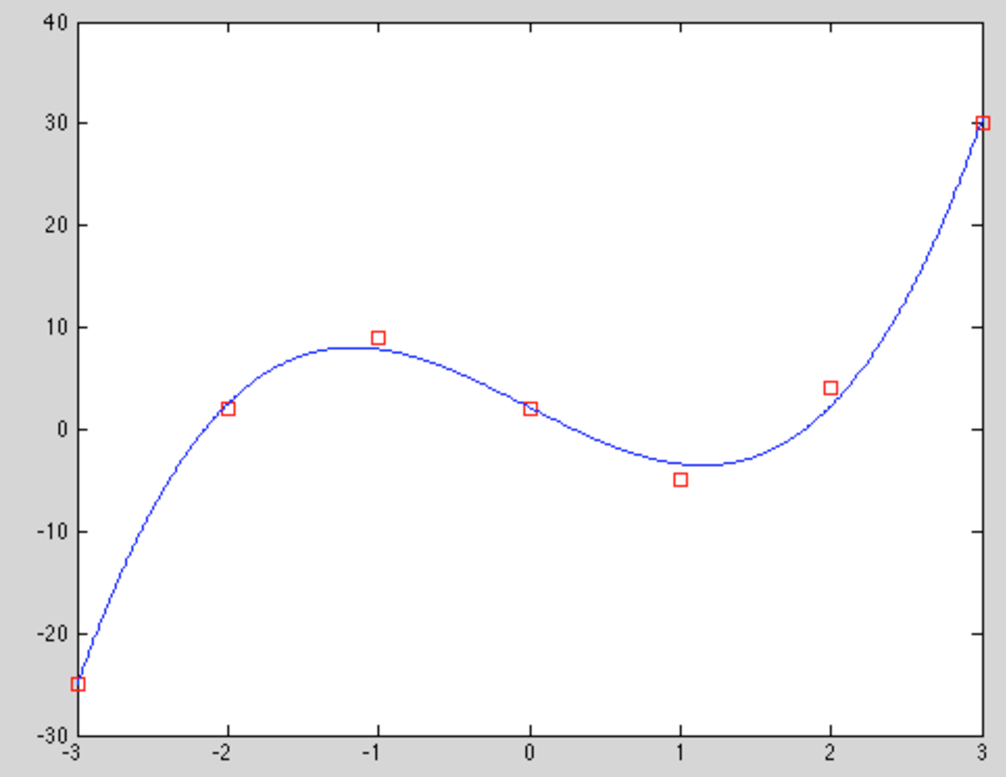
\includegraphics[height=62mm]{assets/figures/exe7fig1serie2.pdf} \hspace{5mm}
   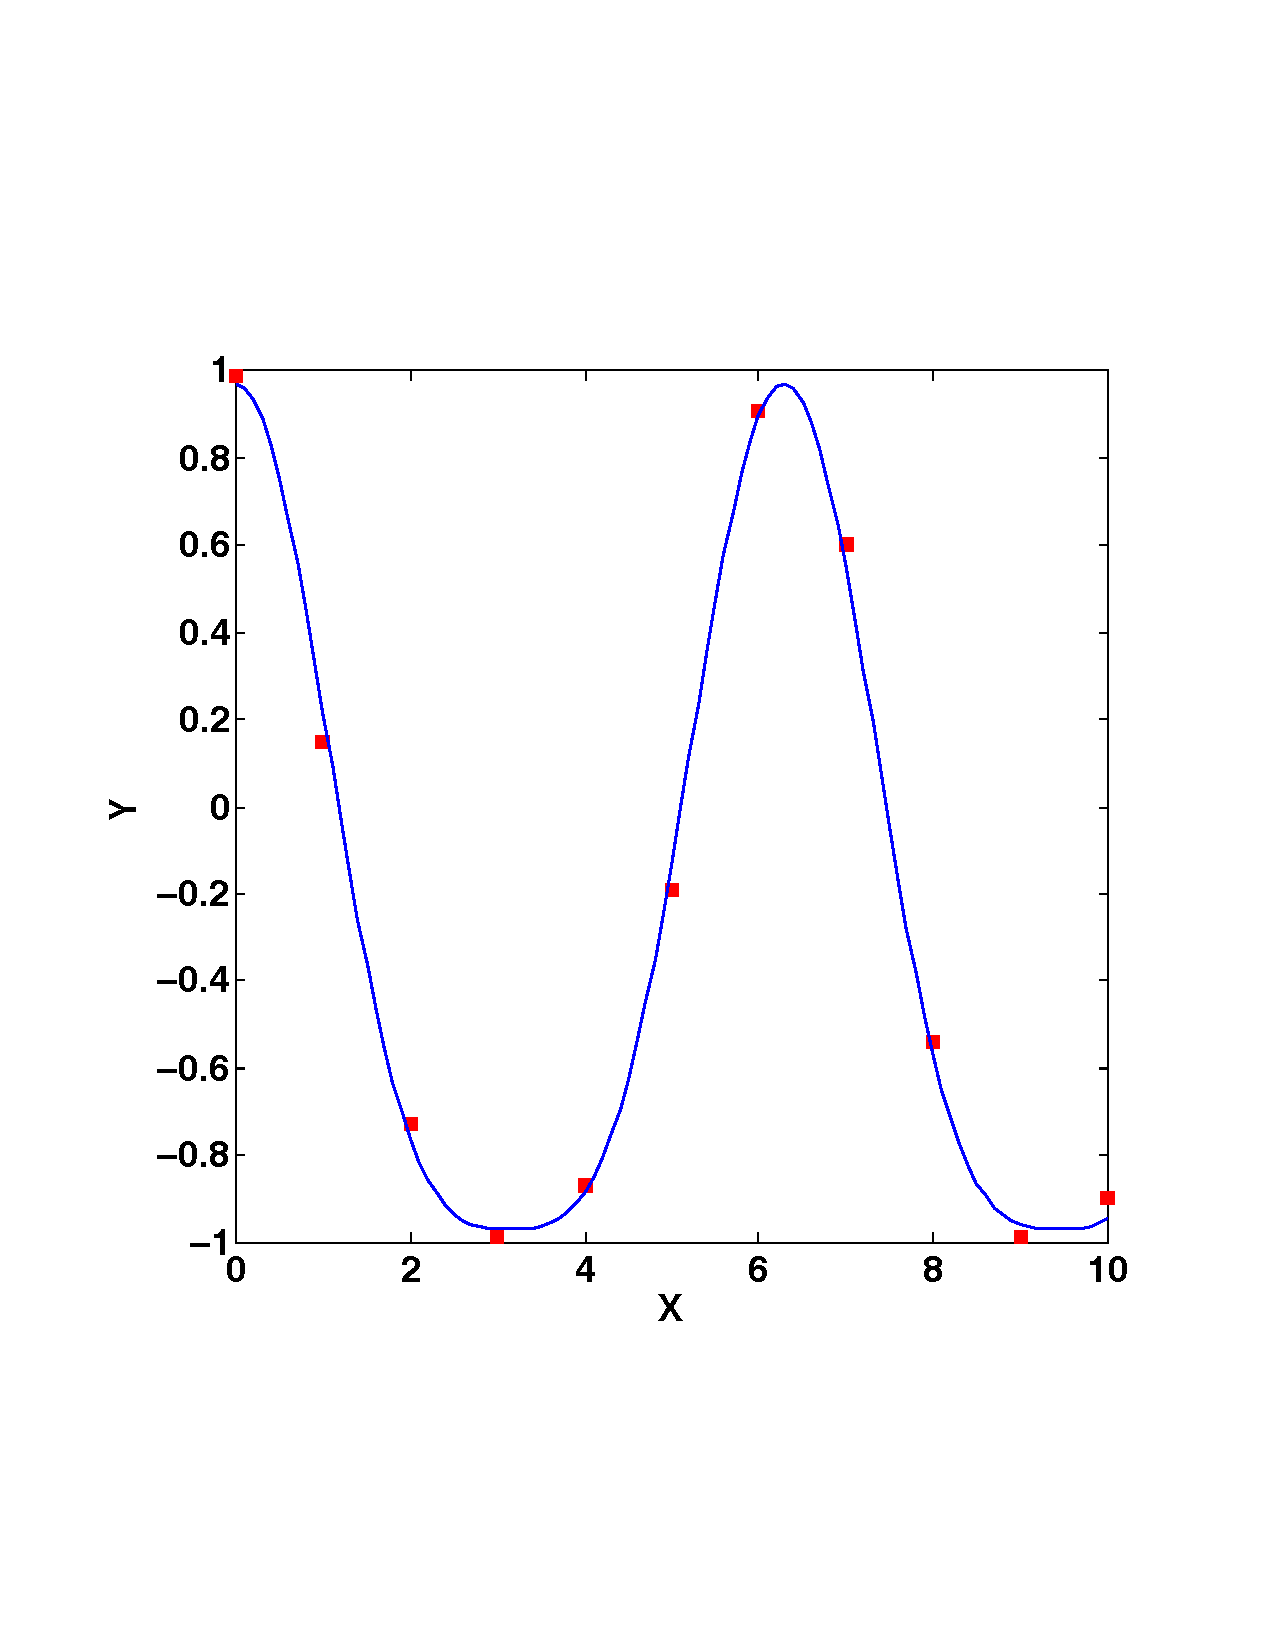
\includegraphics[height=62mm]{assets/figures/exe8fig1serie2.pdf}
   \caption{Solutions des exercices 4.6 (gauche) et 4.7 (droite).}
   \label{fig:exe7}
\end{figure}

%..........
\subsection*{Solution de l'exercice 9.7}
%..........

La théorie est rappelée dans l'exercice 7 de la première série d'exercices. Simplement, alors que dans l'exercice 8 ci-dessus les fonctions $h_j(x)$ sont des fonctions toutes simples de x, ici on aura que $h_1(x)=\cos{x}$ et $h_2(x)=\sin^{2}{x}$. Les coefficients $a$ et $b$ sont donnés par la solution du système
\begin{equation*}
\begin{bmatrix}
\sum_i h_1^2(x_i)       & \sum_i h_2(x_i)h_1(x_i) \\
\sum_i h_1(x_i)h_2(x_i) & \sum_i h_2^2(x_i)
\end{bmatrix}
\begin{bmatrix} a \\ b \end{bmatrix}=
\begin{bmatrix}
\sum_ih_1(x_i)\,y_i\\
\sum_ih_2(x_i)\,y_i
\end{bmatrix}
\end{equation*}
soit
\begin{equation*}
\begin{bmatrix}
\sum_i \cos^2{x_i} & \sum_i \sin^2{x_i}\cos{x_i} \\
\sum_i \cos{x_i}\sin^2{x_i} & \sin^4{x_i}
\end{bmatrix}
\begin{bmatrix} a \\ b \end{bmatrix}=
\begin{bmatrix}
\sum_i\cos{x_i}\,y_i\\
\sum_i\sin^2{x_i}\,y_i
\end{bmatrix}
\end{equation*}
numériquement
\begin{equation*}
\begin{bmatrix}
    5.9986 &  -0.2399 \\
   -0.2399 &   3.6259
\end{bmatrix}
\begin{bmatrix} a \\ b \end{bmatrix}=
\begin{bmatrix} 5.9315 \\ -1.8231 \end{bmatrix}
\end{equation*}
et donc
\begin{equation*}
\begin{bmatrix} a \\ b \end{bmatrix}=
\left(\begin{bmatrix}
    5.9986 &  -0.2399 \\
   -0.2399 &   3.6259
\end{bmatrix}\right)^{-1}
\begin{bmatrix} 5.9315 \\ -1.8231 \end{bmatrix}=
\begin{bmatrix}
0.1671 & 0.0111 \\
0.0111 & 0.2765
\end{bmatrix}
\begin{bmatrix} 5.9315 \\ -1.8231 \end{bmatrix}=
\begin{bmatrix} 0.9713 \\ -0.4385 \end{bmatrix}
\end{equation*}
La solution est proche des valeurs utilisées pour la construction de cet exercice, à savoir $[a,b]=[1,-0.5]$. On montre en figure \ref{fig:exe7} (droite) la superposition de la solution et des points de mesure. L'ajustement est très bon.

%..........
\subsection*{Solution de l'exercice 9.8}
%..........

La théorie est celle de la régression générale, avec, ici, $h_1(\Delta t)=\Delta t$ et $h_2(\Delta t)=1/\Delta t$. On trouve la solution suivante (voir figure \ref{fig:exe9})
\begin{equation*}
\begin{bmatrix} a \\ b \end{bmatrix}=
\left(\begin{bmatrix}
3.85 & 10 \\
  10 & 154.9768
\end{bmatrix}\right)^{-1}
\begin{bmatrix} 29.2020 \\ 205.5244 \end{bmatrix}=
\begin{bmatrix}
    0.3120 &  -0.0201 \\
   -0.0201 &   0.0078
\end{bmatrix}
\begin{bmatrix} 29.2020 \\ 205.5244 \end{bmatrix}=
\begin{bmatrix} 4.9740 \\ 1.0052 \end{bmatrix}
\end{equation*}
Pour trouver le $\Delta t$ optimal, soit la valeur qui minimise l'erreur, on pose la dérivée de $\epsilon$ par rapport à $\Delta t$ égale à zéro,
$$
\frac{\text{d}\epsilon}{\text{d}\Delta t}=a-\frac{b}{\Delta t^2}=0\Longrightarrow
(\Delta t)_{opt}=\sqrt{b/a}=\sqrt{1.0052/4.9740}=0.4495\ \text{ms}
$$
